\documentclass[a4paper, oneside]{article}

\makeatletter
    \renewcommand\paragraph{%
        \@startsection{paragraph}{4}{0mm}%
           {-\baselineskip}%
           {.5\baselineskip}%
           {\normalfont\normalsize\bfseries}}
    \makeatother

\usepackage{../../Stile/mercuryseven}
\usepackage{titlesec}
\usepackage{xcolor}
\newcommand{\Titolo}{Piano Di Progetto}

\newcommand{\VersioneDocumento}{\versPdP}

\newcommand{\ACapoRedazione}{\textit{\Davide{}} \newline \textit{\Francesco{}} \newline{} \textit{\Matteo{}}}

\newcommand{\Verifica}{\textit{\Daniele{}} \newline{} \textit{\Lucrezia{}} \newline{} \textit{\Giosue{}}}

\newcommand{\Responsabile}{\textit{\Tommaso{}}}

\newcommand{\Distribuzione}{\textit{Prof. \Tullio{}} \newline \textit{Prof. \Riccardo{}} \newline Gruppo \textit{\Gruppo{}}}

\newcommand{\Uso}{Esterno}

\newcommand{\DescrizioneDoc}{Descrizione della pianificazione realizzata da \textit{\Gruppo{}}, l'analisi dei rischi che potrebbero verificarsi, il prospetto economico e l'organigramma}

\begin{document}
\copertina{}

\section*{\centerline{Registro delle modifiche}}
{
	\newlength{\freewidth}
	\setlength{\freewidth}{\dimexpr\textwidth-10\tabcolsep}
	\renewcommand{\arraystretch}{1.5}
	\centering
	\setlength{\aboverulesep}{0pt}
	\setlength{\belowrulesep}{0pt}
	\rowcolors{2}{AzzurroGruppo!10}{white}
	\begin{longtable}{C{.131777\freewidth} C{.134036\freewidth} C{.263554\freewidth} C{.188254\freewidth} C{.282379\freewidth}}
		\toprule 
		\rowcolor{AzzurroGruppo!30}
		\textbf{Versione} & \textbf{Data} & \textbf{Autore} & \textbf{Ruolo} & \textbf{Descrizione}\\
		\toprule
		\endhead

		v1.0.0-0.10 & 2021-04-15 & \Matteo{} & \RdP{} & Approvazione del documento. \\
		v0.4.0-0.10 & 2021-04-14 & \Daniele{}, \newline{} \Lucrezia{} & \ver{}, \newline{} \prog{} & Correzione e verifica segnalazioni Product Baseline.\\
		v0.3.0-0.9 & 2021-04-05 & \Daniele{}, \newline{} \Giosue{} & \ver{}, \newline{} \progr{} & Stesura e verifica glossario. \\
		v0.2.1-0.9 & 2021-04-03 & \Davide{}, \newline{} \Lucrezia{} & \ver{}, \newline{} \prog{} & Aggiunta e verifica immagini. \\
		v0.2.0-0.9 & 2021-04-02 & \Davide{}, \newline{} \Giosue{} & \ver{}, \newline{} \progr{} & Stesura e verifica test e archittettura. \\
		v0.1.0-0.9 & 2021-03-30 & \Daniele{}, \newline{} \Giosue{} & \ver{}, \newline{} \progr{} & Stesura e verifica tecnologie e librerie. \\
		v0.0.2-0.9 & 2021-03-26 & \Davide{}, \newline{} \Lucrezia{} & \ver{},\newline{} \prog{} & Stesura e verifica introduzione. \\
		v0.0.1-0.8 & 2021-03-23 & \Davide{},\newline{} \Lucrezia{} & \ver{},\newline{} \prog{} & Stesura e verifica scheletro documento. \\
		\bottomrule
		\hiderowcolors
	\end{longtable}
}
\newpage

\newpage
\tableofcontents
\listoftables
\listoffigures

\newpage
\section{Introduzione}
\subsection{Scopo del documento}
Lo scopo del documento è quello di specificare la pianificazione che \Gruppo  adotterà per sviluppare il progetto \NomeProgetto. All'interno sono presenti le strategie per la gestione dei rischi, le suddivisioni dei compiti con il relativo preventivo dell'utilizzo delle risorse, e il modello di sviluppo secondo il quale il team ha intenzione di lavorare.
In particolare il documento tratta i seguenti argomenti:
\begin{itemize}
\item analisi dei rischi;
\item descrizione del modello di sviluppo;
\item pianificazione delle attività e divisione dei ruoli;
\item stima dei costi e delle risorse necessarie allo sviluppo del progetto.
\end{itemize}
\subsection{Scopo del prodotto}
L'obbiettivo del progetto è quello di sviluppare un algoritmo in grado di garantire la sincronizzazione e il salvataggio di file tra server e client, appoggiandosi sul servizio \textit{Zextras Drive}.
L'interfaccia deve essere multi piattaforma, per poter essere utilizzato nei più importanti sistemi operativi desktop esistenti.
Inoltre, il prodotto deve essere sviluppato aderendo al pattern MVC, così da permettere rapidi cambiamenti della Business logic o dell'interfaccia utenti senza eccessivo sviluppo aggiunto.
\subsection{\G{}}
Al fine di rendere il documento più chiaro e leggibile, si fornisce il \textit{Glossario}. In questo documento saranno contenuti e descritti tutti i termini che potrebbero risultare ambigui o con un significato particolare. I termini saranno contrassegnati da una 'G' a pedice.
\subsection{Riferimenti}
\subsubsection{Normativi}
\begin{itemize}
\item \NdP{};
\item \textbf{Regolamento Organigramma e specifica tecnico-economica:} \url{https://www.math.unipd.it/~tullio/IS-1/2020/Progetto/RO.html}.
\end{itemize}

\subsubsection{Informativi}
\begin{itemize}
\item \textbf{Capitolato d'appalto:} \url{https://www.math.unipd.it/~tullio/IS-1/2020/Progetto/C7.pdf};
\item\textbf{Software Engineering - Ian Sommerville - 9th Edition, 2010;}
\item \textbf{Slide L05 del corso Ingegneria del Software - Ciclo di vita del software:} \url{https://www.math.unipd.it/~tullio/IS-1/2020/Dispense/L05.pdf};
\item \textbf{Slide L06 del corso Ingegneria del Software - Gestione di Progetto:} \url{https://www.math.unipd.it/~tullio/IS-1/2020/Dispense/L06.pdf}.
\end{itemize}

\subsection{Scadenze}
Il gruppo \Gruppo si impegna a rispettare le seguenti scadenze per lo sviluppo del progetto \NomeProgetto:
\begin{itemize}
\item \textbf{Revisione dei Requisiti:} 2021-01-18;
\item \textbf{Revisione di Progettazione:} 2021-03-08;
\item \textbf{Revisione di Qualifica:} 2021-04-09;
\item \textbf{Revisione di Accettazione:} 2021-05-10.
\end{itemize}
\newpage
\section{Analisi dei Rischi}
Durante lo sviluppo di un progetto la probabilità che si verifichino delle criticità è alta, 
soprattutto quando si tratta di progetti complessi e/o di grandi dimensioni, per questo motivo
un'attenta analisi dei rischi può aiutare ad evitare o quantomeno a gestire al meglio tali criticità.
Il piano di gestione dei rischi si suddivide in 4 attività:
\begin{itemize}
    \item \textbf{Individuazione dei rischi}: \textit{TODO;}
    \item \textbf{Analisi dei rischi}: \textit{TODO;}
    \item \textbf{Pianificazione di controllo}: \textit{TODO;}
    \item \textbf{Monitoraggio dei rischi}: \textit{TODO.}
\end{itemize}
Abbiamo suddiviso i pricipali fattori di rischio nelle seguenti categorie:
\begin{itemize}
    \item Rischi legati alle tecnologie
    \item Rischi legati all’organizzazione
    \item Rischi legati alle persone
\end{itemize}

\subsection{Rischi legati alle tecnologie}

\paragraph{Inesperienza Tecnologica}
\renewcommand{\arraystretch}{1}
	\begin{table}[H]
		\begin{center}
			\setlength{\aboverulesep}{0pt}
			\setlength{\belowrulesep}{0pt}
			\setlength{\extrarowheight}{.75ex}
			\rowcolors{2}{AzzurroGruppo!10}{white}
			\begin{tabular}{ c c }
				\rowcolor{AzzurroGruppo!30} 
				%\textbf{Prima colonna} & \textbf{Seconda colonna}  \\
                \toprule
                Descrizione & Il team presanta un'esperienza eterogenea e superficiale nell'utilizzo di molte tecnologie richieste in questo progetto. \\
				Conseguenze & Potrebbe comportare l'insorgere di problemi operativi o ritardi dovuti ai tempi di apprendimento soggettivi. \\
                Occorrenza & Media \\
                Prericolosità & Media \\
                Precauzioni & Il \textit(Responsabile di progetto) si occuperà di suddividere il carico di lavoro in modo bilanciato, tenendo conto delle capacità del singolo individuo. Ogni membro del team dovrà quindi preoccuparsi di segnalare le sue conoscenze preliminari al \textit(Responsabile di progetto). \\
                Piano di contingenza & Ogni membro del team avrà cura di prendere dimestichezza con le tecnologie impiegate in modo tale da diventare il più possibile autonomo nel proprio lavoro. I compiti più complessi saranno affidati a più membri in modo tale da velocizzare i tempi di sviluppo e favorire l'aiuto reciproco. \\
				\bottomrule
			\end{tabular}
			\caption{Tabella dettaglio rischio di Inesperienza Tecnologica}
		\end{center}
    \end{table}

\paragraph{Problematiche Hardware}
\renewcommand{\arraystretch}{1}
    \begin{table}[H]
        \begin{center}
            \setlength{\aboverulesep}{0pt}
            \setlength{\belowrulesep}{0pt}
            \setlength{\extrarowheight}{.75ex}
            \rowcolors{2}{AzzurroGruppo!10}{white}
            \begin{tabular}{ c c }
                \rowcolor{AzzurroGruppo!30} 
                %\textbf{Prima colonna} & \textbf{Seconda colonna}  \\
                \toprule
                Descrizione & Ogni membro del team lavora allo sviluppo utilizzando il proprio computer personale, quest'ultimo può essere soggetto a malfunzionamenti. \\
                Conseguenze & Il guasto di uno o più computer porterebbe ad una parziale perdita di dati causando ritardi. Sebbene remota esiste anche la possibilità di una totale perdita di dati qualora l'avaria avvenisse in tutti i computer contemporaneamnte. \\
                Occorrenza & Bassa \\
                Prericolosità & Alta \\
                Precauzioni & Ogni membro del team si adopererà per eseguire backup frequenti durante il processo di sviluppo e mantenere operativo il proprio hardware. \\
                Piano di contingenza & Nel caso in cui si verifichi un problema hardware bisognerà procedere a riparare il danno il più rapidamente possibile. A seconda delle norme sulla mobilità vigenti, sarà possibile utilizzare i computer messi a diposizione nei laboratori informatici dell'Ateneo. \\
                \bottomrule
            \end{tabular}
            \caption{Tabella dettaglio rischio di Problematiche Hardware}
        \end{center}
    \end{table}

\paragraph{Problematiche Software}
\renewcommand{\arraystretch}{1}
    \begin{table}[H]
        \begin{center}
            \setlength{\aboverulesep}{0pt}
            \setlength{\belowrulesep}{0pt}
            \setlength{\extrarowheight}{.75ex}
            \rowcolors{2}{AzzurroGruppo!10}{white}
            \begin{tabular}{ c c }
                \rowcolor{AzzurroGruppo!30} 
                %\textbf{Prima colonna} & \textbf{Seconda colonna}  \\
                \toprule
                Descrizione & il team si avvale di servizi e software di terze parti per la gestione dei documenti e della \glossary{codebase}. La buona gestione di questi ultimi non è competenza del team. \\
                Conseguenze & Eventuali disservizi potrebbero causare gravi perdite di dati e ritardi. \\
                Occorrenza & Bassa \\
                Prericolosità & Alta \\
                Precauzioni & Ogni membro del team si impegnerà a tenere aggiornato un backup locale di tutti i \glossary{repository} remoti. \\
                Piano di contingenza & Il \textit{Responsabile di progetto} avrà cura di cercare altri servizi simili ai precedenti e più affidabili. \\
                \bottomrule
            \end{tabular}
            \caption{Tabella dettaglio rischio di Problematiche Software}
        \end{center}
    \end{table}

\subsection{Rischi legati all’organizzazione}

\paragraph{TODO}
\renewcommand{\arraystretch}{1}
    \begin{table}[H]
        \begin{center}
            \setlength{\aboverulesep}{0pt}
            \setlength{\belowrulesep}{0pt}
            \setlength{\extrarowheight}{.75ex}
            \rowcolors{2}{AzzurroGruppo!10}{white}
            \begin{tabular}{ c c }
                \rowcolor{AzzurroGruppo!30} 
                %\textbf{Prima colonna} & \textbf{Seconda colonna}  \\
                \toprule
                Descrizione & TODO \\
                Conseguenze & TODO \\
                Occorrenza & TODO \\
                Prericolosità & TODO \\
                Precauzioni & TODO \\
                Piano di contingenza & TODO \\
                \bottomrule
            \end{tabular}
            \caption{Tabella dettaglio rischio di TODO}
        \end{center}
    \end{table}

\subsection{Rischi legati alle persone}

\paragraph{TODO}
\renewcommand{\arraystretch}{1}
    \begin{table}[H]
        \begin{center}
            \setlength{\aboverulesep}{0pt}
            \setlength{\belowrulesep}{0pt}
            \setlength{\extrarowheight}{.75ex}
            \rowcolors{2}{AzzurroGruppo!10}{white}
            \begin{tabular}{ c c }
                \rowcolor{AzzurroGruppo!30} 
                %\textbf{Prima colonna} & \textbf{Seconda colonna}  \\
                \toprule
                Descrizione & TODO \\
                Conseguenze & TODO \\
                Occorrenza & TODO \\
                Prericolosità & TODO \\
                Precauzioni & TODO \\
                Piano di contingenza & TODO \\
                \bottomrule
            \end{tabular}
            \caption{Tabella dettaglio rischio di TODO}
        \end{center}
    \end{table}
\newpage
\section{Modello di sviluppo }

Come \glo{team} di sviluppo dobbiamo poter garantire in ogni momento la qualità del prodotto \glo{software} e la sua conformità rispetto ai \glo{requisiti}. \newline
Il modello \glo{iterativo} permette un ciclo evolutivo più flessibile e favorisce il dialogo con gli \glo{stackholder}, adattandosi più facilmente alle esigenze. \newline 
Per tali motivi abbiamo deciso di adottare questo tipo di modello, riducendo i rischi e producendo nuovo valore ad ogni iterazione.

%info
%https://medium.com/geekandjob-blog/scrum-cos%C3%A8-e-come-funziona-metodologia-agile-7c8988feec01
\subsection{Modello Agile}
Il modello di sviluppo \glo{agile} permette di progredire tramite cicli iterativi e incrementali, detti sprint.
É un modello altamente dinamico basato su di un manifesto concepito per evitare un'eccessiva rigidità e valorizzare le risorse disponibili. \newline
Il manifesto contiene questi quattro principi fondanti:

\begin{enumerate}
    \item \textbf{Gli individui e le interazioni più che i processi e gli strumenti}: le persone che fanno parte del progetto producono valore e sono una grande risorsa diponibile;
    \item \textbf{Il software funzionante più che la documentazione esaustiva}: la documentazione va snellita e resa più flessibile senza però perderne in qualità, allocando più risorse al \glo{software}
    \item \textbf{La collaborazione col cliente più che la negoziazione dei contratti}: un contratto inflessibile può essere una potenziale perdità di valore per gli \glo{attori} coinvolti. Va quindi incentivata l’interazione con gli \glo{stakeholder} durante lo sviluppo del progetto;
    \item \textbf{Rispondere al cambiamento più che seguire un piano}: i cambiamenti sono probabili durante lo sviluppo di grandi progetti per questo pianificare tutto fin dall'inizio potrebbe essere uno spreco di risorse.
\end{enumerate}

% FIXME compila con rientro sfasato
L’idea di base per implementare tali principi è l’utilizzo del \textbf{\glo{Product Backlog}}, che cresce man mano che il prodotto viene costruito. \newline
Il lavoro viene quindi suddiviso in piccole funzionalità chiamate \textbf{\glo{User Story}} le quali poi vengono selezionate per essere portate a ternime negli \textbf{sprint}, venendo, di fatto, sviluppate indipendentemente in una sequenza continua dall’analisi all’integrazione. \newline

Gli obiettivi strategici sono quindi:
\begin{itemize}
    \item poter costantemente e in ogni momento dimostrare al cliente ciò che è stato fatto;
    \item verificare l’avanzamento tramite il progresso reale dello sviluppo;
    \item soddisfare e motivare gli sviluppatori con risultati immediati;
    \item assicurare e dimostrare una buona \glo{verifica} e integrazione dell’intero prodotto \glo{software}.
\end{itemize}


\begin{figure}[H]
    \centering
    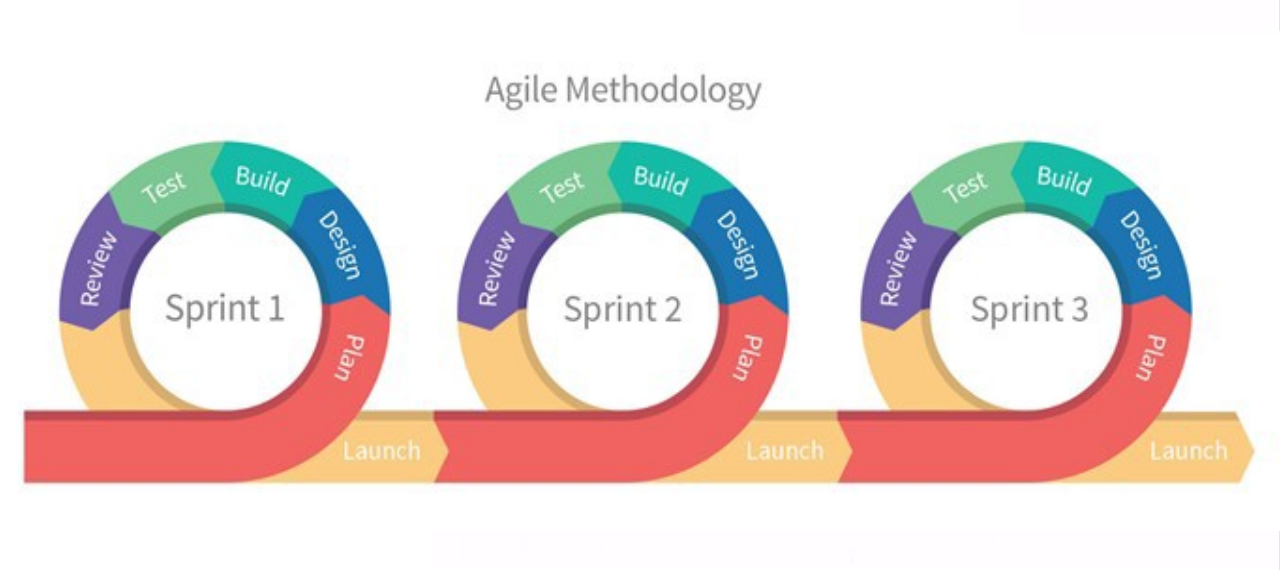
\includegraphics[scale = 0.25]{components/img/agile.png}
    \caption{Rappresentazione del modello agile}
    \label{fig:Rappresentazione del modello agile}
\end{figure}
\newpage
\section{Pianificazione}
La fase di pianificazione consiste nella suddivisione del lavoro tra i vari componenti del gruppo \Gruppo . La suddivisione deve essere equa e deve fare in modo che ogni componente abbia la possibilità di ricoprire almeno una volta tutti i ruoli.
Sono stati determinati cinque periodi principali per suddividere il lavoro:
\begin{itemize}
\item analisi;
\item consolidamento dei \glo{requisiti};
\item progettazione architetturale;
\item progettazione di dettaglio e codifica;
\item \glo{validazione} e collaudo.
\end{itemize}
Ognuno di questi viene poi suddiviso in diversi \glo{sprint} dove vengono individuate le attività che verranno realizzate.
Infine, ogni periodo viene riassunto nel corrispettivo \glo{diagramma di Gantt}.
\subsection{Analisi}
Questo periodo ha inizio il 2020-11-09 procede con quattro fasi fino al 2021-01-11.
Durante il suo decorso i ruoli attivi sono:
\begin{itemize}
\item \textit{responsabile};
\item \textit{amministratore};
\item \textit{analista};
\item \textit{verificatore}.
\end{itemize}
Le precondizioni sono:
\begin{itemize}
	\item formazione del gruppo;
	\item presentazione dei capitolati.
\end{itemize}
Le post condizioni sono:
\begin{itemize}
	\item scelta del nome e del logo del gruppo;
	\item creazione della e-mail;
	\item scelta del capitolato su cui svolgere il progetto;
	\item redazione dei documenti quali: \SdF{}, \NdP{}, \PdP{}, \G{}, \LdP{}, \PdQ{}, \AdR{} e i verbali;
	\item \glo{verifica} e approvazione dei documenti.
\end{itemize}
\subsubsection{Attività}
Questo periodo è composto da sette attività che corrispondono alla produzione dei seguenti documenti:
\begin{itemize}
	\item \textbf{Studio di Fattibilità:} viene fatta una discussione su ogni capitolato, rilevandone pro e contro di ognuno di essi, e dopo un periodo di studio e analisi il gruppo pone la sua preferenza in uno dei capitolati proposti;
	\item \textbf{Norme di Progetto:} vengono definite tutte le regole che il gruppo dovrà rispettare durante lo sviluppo del progetto, tra cui norme relative al prodotto da realizzare e ai processi da adottare;
	\item \textbf{Individuazione degli strumenti:} consiste nel determinare quali strumenti devono essere utilizzati dal gruppo; vengono ricercati strumenti per la comunicazione, per la stesura dei documenti, per lo sviluppo e la \glo{verifica} del \glo{software};
	\item \textbf{Analisi dei \glo{Requisiti}:} viene analizzato il capitolato scelto nell'attività di \SdF{} e vengono identificanti i \glo{requisiti} del capitolato; il documento viene composto dagli \textit{analisti};
	\item \textbf{Piano di Progetto:} Attività di pianificazione dei compiti e suddivisione dei ruoli dove viene calcolato il preventivo per la realizzazione di progetto; il documento viene composto dal \textit{responsabile};
	\item \textbf{Piano di Qualifica:} si individuano i metodi necessari per garantire la qualità del prodotto; viene redatto dall'\textit{amministratore} e dal \textit{progettista};
	\item\textbf{Glossario:} si individuano tutti i termini che possono risultare ambigui e vengono affiancati da una definizione all'interno del documento;  
	\item \textbf{Lettera di Presentazione:} Documento in cui il gruppo \Gruppo{} si candida come fornitore del prodotto \glo{software} richiesto.
\end{itemize}
\subsubsection{Sprint}
La pianificazione di questo periodo è stata suddivisa nei seguenti \glo{sprint}:
\begin{itemize}
	\item \textbf{\glo{Sprint} 1, dal 2020-11-24 al 2020-12-07:}
	\begin{itemize}
	\item vengono prese decisioni riguardanti: il nome del \glo{team}, l'indirizzo e-mail, il logo, la frequenza degli incontri e gli strumenti per la comunicazione;
	\item viene svolta la discussione sui capitolati, esponendo le preferenze personali dei membri del gruppo. Viene, quindi, svolta l'analisi dei capitolati dove, per ognuno di essi, vengono esaminati pro e contro e vengono effettuate delle valutazioni sui rischi. Successivamente può iniziare la stesura dello Studio di Fattibilità;
	\item viene iniziata la stesura delle \NdP{} per fissare le regole delle attività del gruppo;
	\item inizio della stesura del \PdP{}, dove viene descritta la pianificazione del lavoro da svolgere e la suddivisione dei ruoli tra i membri del gruppo;
	\item vengono stesi i verbali interni relativi alle riunioni del gruppo.
	\end{itemize}
	\item \textbf{\glo{Sprint} 2, dal 2020-12-08 al 2020-12-22:}
	\begin{itemize}
		\item viene conclusa la stesura delle \NdP{};
		\item viene conclusa la stesura del \PdP{}, eccetto il consuntivo;
		\item inizio stesura del \textit{Glossario}, registrando i termini usati nei documenti che risultano ambigui;
		\item vengono stesi i verbali interni relativi agli incontri svolti durante questo \glo{sprint}.
	\end{itemize}
	\item \textbf{\glo{Sprint} 3, dal 2020-12-23 al 2021-01-04:}
	\begin{itemize}
		\item il gruppo inizia ad analizzare il capitolato scelto, ricercando i \glo{requisiti} e procedendo con la stesura dell'\AdR{};
		\item Si procede con la stesura del \PdQ{}, individuando i metodi per garantire la qualità del prodotto;
		\item stesura della \textit{Lettera di Presentazione};
		\item vengono stesi i verbali interni relativi agli incontri svolti durante questo \glo{sprint}.
	\end{itemize}
	\item \textbf{dal 2021-01-05 al 2021-01-11 :}
	\begin{itemize}
		\item viene completata la stesura del \textit{Glossario};
		\item viene completata la stesura del \AdR{};
		\item il gruppo uniforma tutti i documenti prodotti alle regole stabilite nelle \NdP{} se necessario;
		\item viene steso il consuntivo finale riguardante il periodo effettuato;
		\item vengono svolte le ultime attività di \glo{verifica} sui documenti.
	\end{itemize}
\end{itemize}

\subsubsection{Diagramma di Gantt: analisi}
\begin{figure}[H]
    \centering
    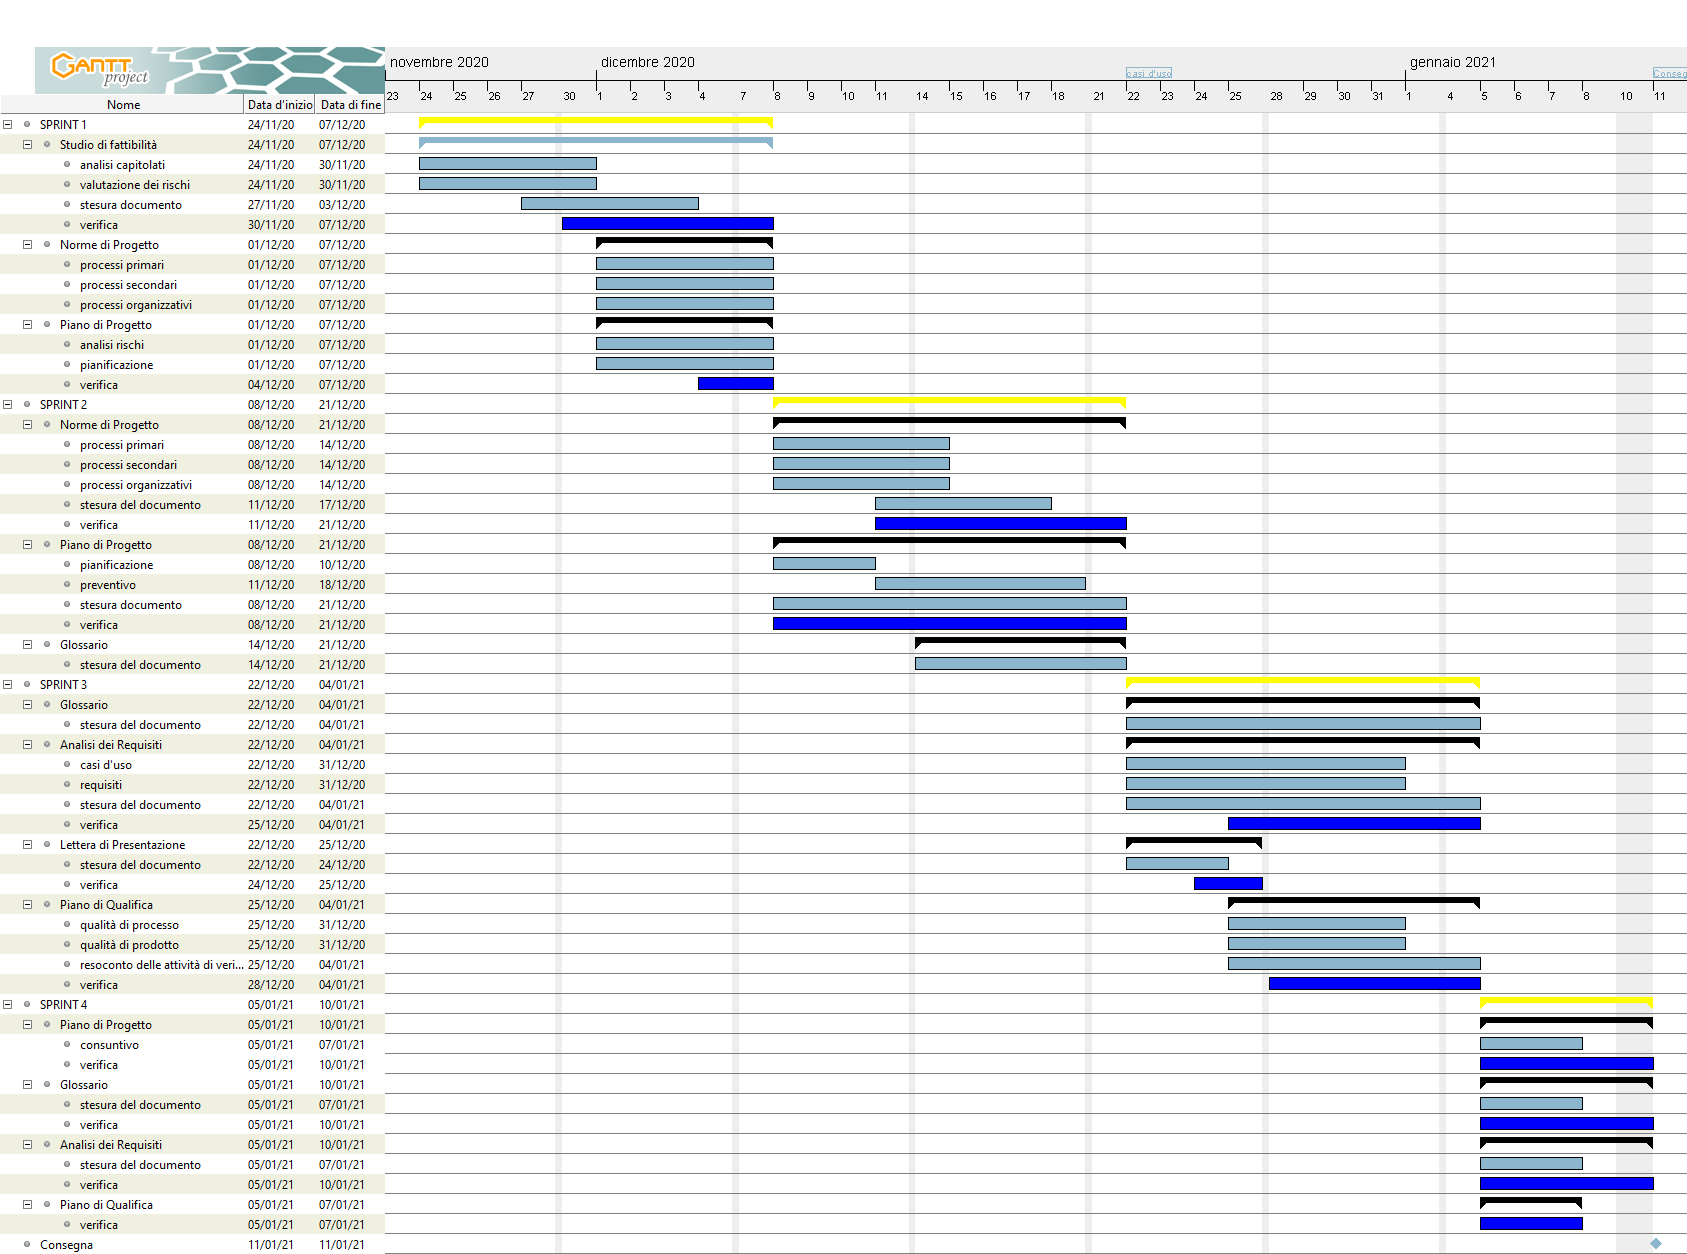
\includegraphics[scale = 0.25]{components/img/Analisi.png}
    \caption{Diagramma di Gantt della fase di Analisi}
    \label{fig:Diagramma di Gantt, fase di Analisi}
\end{figure}

\newpage
\subsection{Consolidamento dei Requisiti}
Questo periodo ha inizio il 2021-01-12 e si conclude il 2021-01-18.
le precondizioni sono:
\begin{itemize}
	\item le post condizioni della fase precedente;
	\item consegna dei documenti richiesti.
\end{itemize}
Le post condizioni sono:
\begin{itemize}
	\item conclusione della preparazione della presentazione da esporre per la Revisione dei \ignore{Requisiti};
	\item i componenti devono essere preparati per l'utilizzo delle tecnologie necessarie.
\end{itemize}
\subsubsection{Attività}
Le attività che vengono svolte sono:
\begin{itemize}
	\item miglioramento dei documenti e \glo{verifica};
	\item preparazione alla presentazione per la Revisione dei \ignore{Requisiti};
	\item studio autonomo che ogni componente dovrà effettuare per approfondire le tecnologie necessarie nelle prossime fasi.
\end{itemize}
\subsubsection{Diagramma di Gantt: Consolidamento dei Requisiti}
\begin{figure}[H]
    \centering
    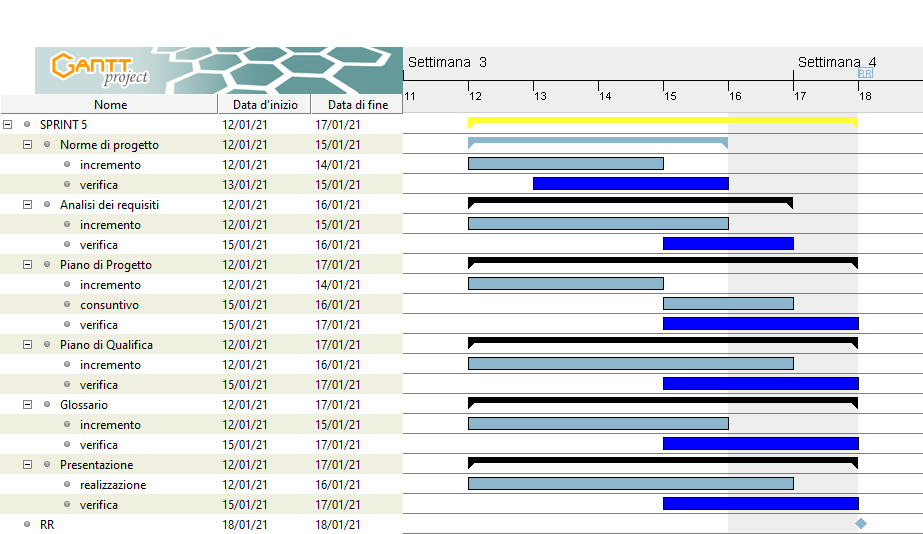
\includegraphics[scale = 0.4]{components/img/consolidamento_requisiti.png}
    \caption{Diagramma di Gantt della fase di Consolidamento dei Requisiti}
    \label{fig:Diagramma di Gantt, fase di Consolidamento dei Requisiti}
\end{figure}

\newpage
\subsection{Progettazione architetturale}
Questo periodo ha inizio il 2021-01-19 e si conclude il 2021-03-08.
Le precondizioni sono:
\begin{itemize}
	\item le post condizioni del periodo precedente;
	\item è stata approvata la candidatura del gruppo al progetto \NomeProgetto.
\end{itemize}
Le post condizioni sono:
\begin{itemize}
	\item correzione ed incremento dei documenti documenti già prodotti;
	\item produzione del \textit{\glo{Proof of Concept}} e dell'Allegato Tecnico;
	\item completamento della progettazione ad alto livello del \glo{software};
	\item consegna dei documenti richiesti alla Revisione di Progettazione; 	
	\item conclusa la preparazione della presentazione da esporre in sede di revisione.
\end{itemize}
\subsubsection{Attività}
Le attività da svolgere durante il periodo sono:
\begin{itemize}
	\item \textbf{Incremento e \glo{Verifica}:} i documenti già prodotti vengono migliorati e aggiornati se necessario (\NdP{}, \PdP{}, \G{}, \PdQ{}, \AdR{});
	\item \textbf{Technology Baseline:} viene fatta un'analisi ad alto livello del \glo{software} e viene redatto l'Allegato Tecnico dove vengono individuati i design pattern che verranno adottati per lo sviluppo. Infine, viene codificato il \textit{\glo{Proof of Concept}}, il quale viene presentato o condiviso al committente e al \glo{proponente} in una data da definirsi.
\end{itemize}
\subsubsection{Diagramma di Gantt: progettazione architetturale}
\begin{figure}[H]
    \centering
    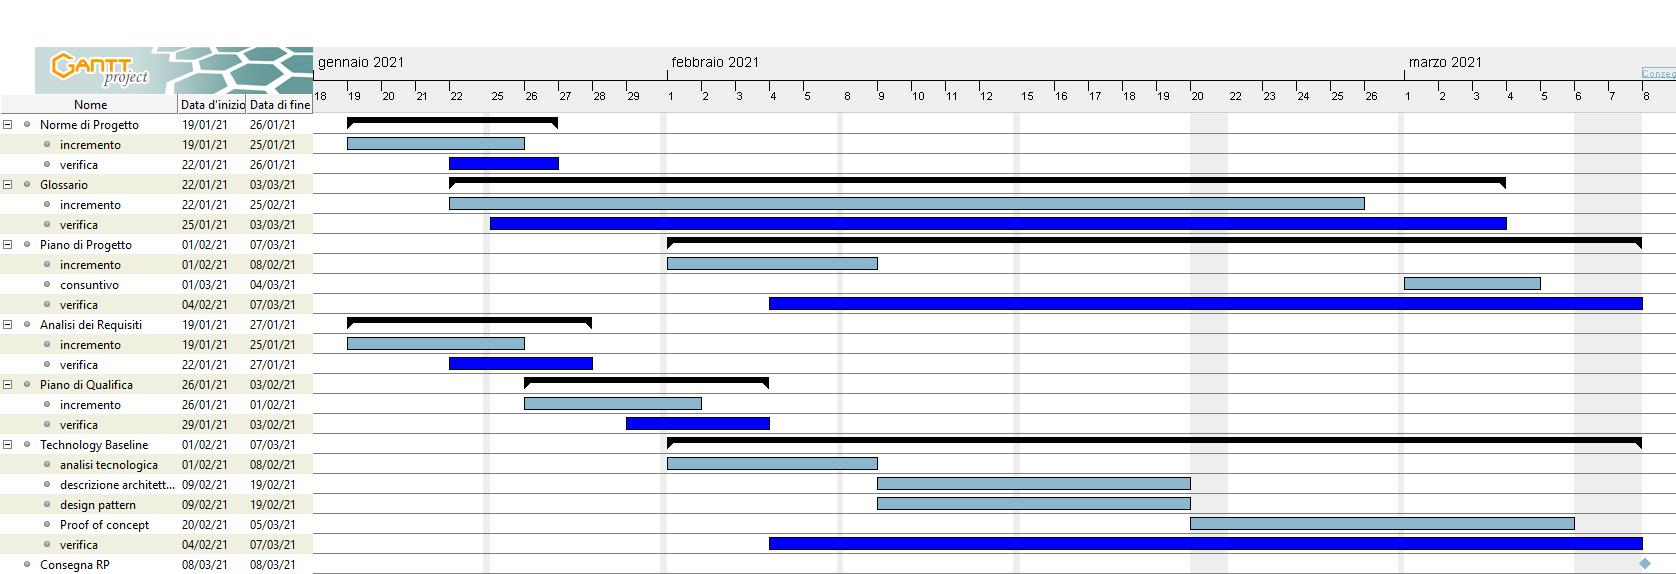
\includegraphics[scale = 0.25]{components/img/progettazione_architetturale.jpg}
    \caption{Diagramma di Gantt della fase di Progettazione Architetturale}
    \label{fig:Diagramma di Gantt, fase di Progettazione Architetturale}
\end{figure}

\newpage
\subsection{Progettazione di dettaglio e codifica}
Questo periodo ha inizio il 2021-03-09 e si conclude il 2021-04-09.
Le precondizioni sono:
\begin{itemize}
	\item aggiornamento e correzione dei documenti;
	\item definizione dell'architettura ad alto livello per il \glo{software};
	\item  superamento del colloquio per la \textit{Technology Baseline}.
\end{itemize}
Le post condizioni sono:
\begin{itemize}
	\item aggiornamento e correzione dei documenti;
	\item stesura del \textit{Manuale Utente};
	\item stesura della \textit{Specifica Tecnica};
	\item superamento del colloquio per la \textit{Product Baseline};
	\item completamento della codifica e della relativa \glo{verifica} del prodotto \glo{software}.
\end{itemize}
\subsubsection{Attività}
Le attività che vengono svolte sono:
\begin{itemize}
	\item \textbf{Incremento e \glo{verifica}:} vengono aggiornati e migliorati i documenti(\NdP{}, \PdP{}, \G{}, \PdQ{}, \AdR{}, \textit{Technology Baseline});
	\item \textbf{Product Baseline:} segue la \textit{Technology Baseline}, vengono analizzate più in dettaglio le \glo{unità} i design pattern, le classi e le attività necessarie alla codifica;
	\item \textbf{Specifica Tecnica:} documento contenente tutte le caratteristiche del prodotto e le motivazioni che hanno portato alla loro scelta;
	\item \textbf{Codifica:} questa attività consiste nella scrittura del codice e della sua \glo{verifica};
	\item \textbf{Manuale Utente:} viene redatto un documento che descrive tutte le istruzioni d'uso per l'utente.
\end{itemize}
\subsubsection{Diagramma di Gantt: progettazione di dettaglio e codifica}
\begin{figure}[H]
    \centering
    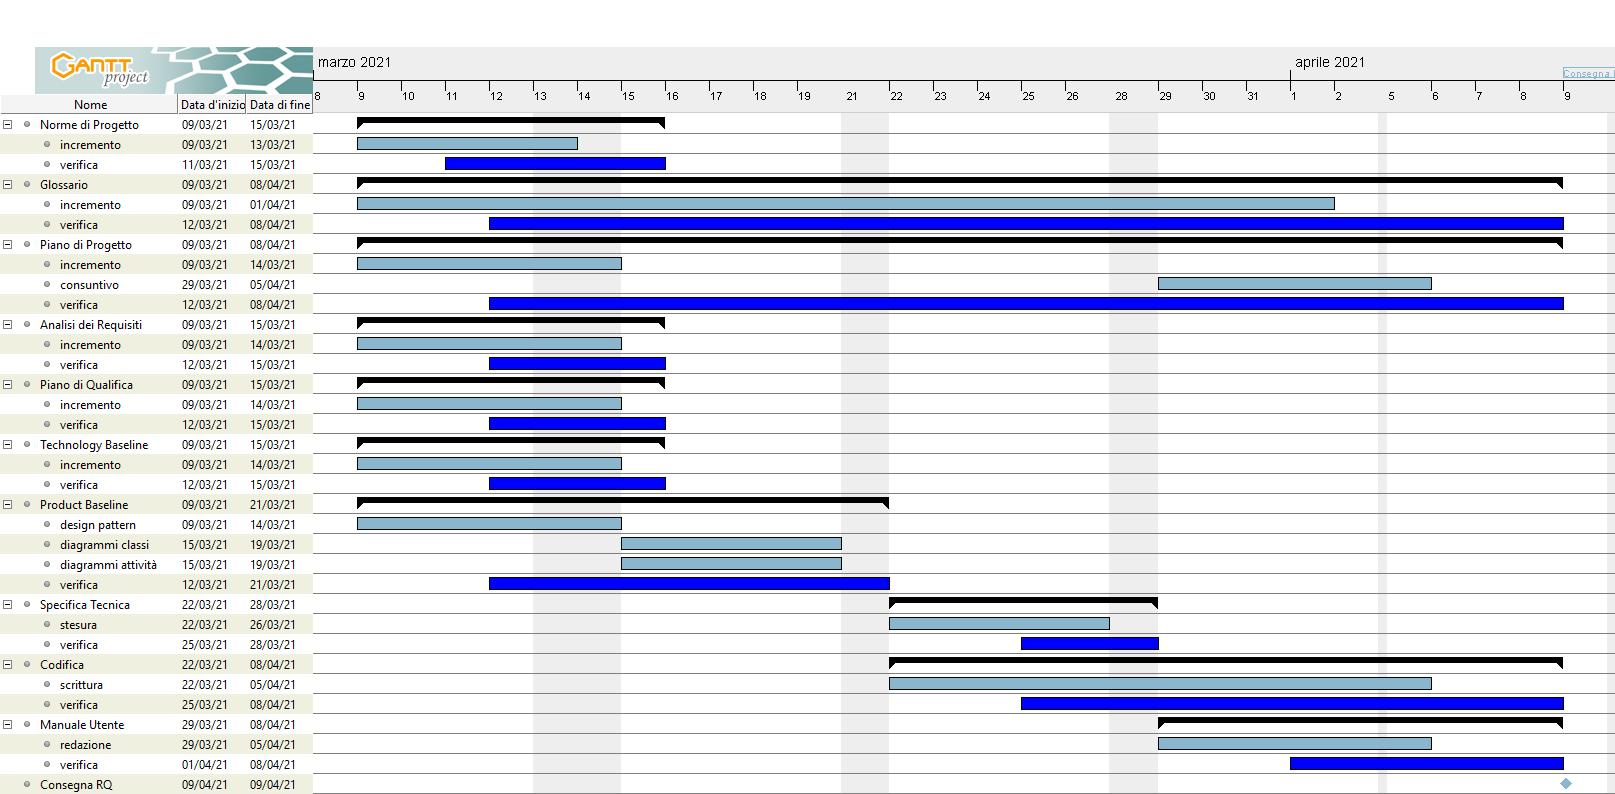
\includegraphics[scale = 0.25]{components/img/progettazione_dettaglio_codifica.jpg}
    \caption{Diagramma di Gantt della fase di Progettazione di Dettaglio e Codifica}
    \label{fig:Diagramma di Gantt, fase di Progettazione di dettaglio e codifica}
\end{figure}

\newpage
\subsection{Validazione e collaudo}
Questo periodo ha inizio il 2021-04-10 e si conclude il 2021-05-10.
Le precondizioni sono:
\begin{itemize}
	\item superamento del colloquio per la Product Baseline;
	\item aggiornamento e correzione dei documenti;
	\item raggiungimento di un prodotto completo, funzionante e di qualità.
\end{itemize}
Le post condizioni sono:
\begin{itemize}
	\item aggiornamento e correzione dei documenti;
	\item stesura del \textit{Manuale Sviluppatore};
	\item esecuzione dei \glo{test} di \glo{sistema} e di accettazione;
	\item consegna dei documenti richiesti alla Revisione di Accettazione.
\end{itemize}
\subsubsection{Attività}
Le attività che vengono svolte sono:
\begin{itemize}
	\item \textbf{Incremento e \glo{verifica}:} vengono migliorati e aggiornati i documenti già prodotti (\NdP{}, \PdP{}, \G{}, \PdQ{}, \AdR{}, \textit{Technology Baseline}, \textit{Product Baseline}, \textit{Specifica Tecnica},\textit{Manuale Utente});
	\item \textbf{\glo{Validazione} e collaudo:} vengono eseguite ulteriori \glo{test} sul prodotto, in modo da garantire la correttezza e un buon livello di qualità;
	\item \textbf{Manuale Sviluppatore:} viene redatto il \textit{Manuale Sviluppatore} atto a fornire tutte le informazione necessarie al mantenimento, manutenzione e ampliamento del prodotto.
\end{itemize}
\subsubsection{Diagramma di Gantt: validazione e collaudo}
\begin{figure}[H]
    \centering
    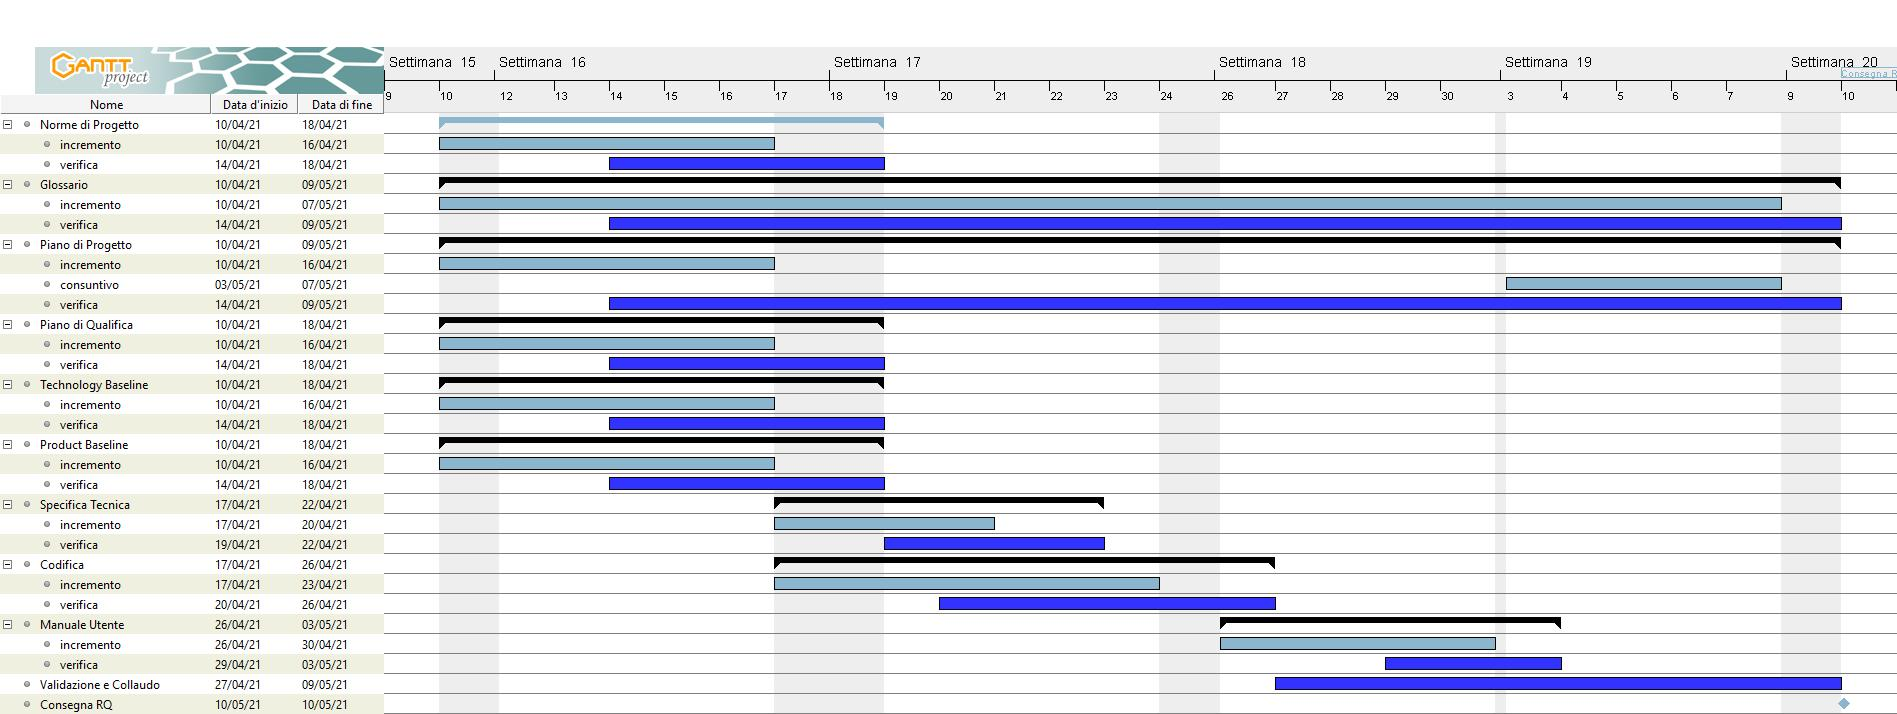
\includegraphics[scale = 0.25]{components/img/validazione_collaudo.jpg}
    \caption{Diagramma di Gantt della fase di Progettazione di Validazione e Collaudo}
    \label{fig:Diagramma di Gantt, fase di Validazione e collaudo}
\end{figure}

\newpage
\section{Preventivo}
Per facilitare la lettura delle seguenti tabelle, vengono utilizzate delle sigle 
per identificare i ruoli:

\begin{table}[H]
		\begin{center}
			\setlength{\aboverulesep}{0pt}
			\setlength{\belowrulesep}{0pt}
			\setlength{\extrarowheight}{.75ex}
			\rowcolors{2}{AzzurroGruppo!10}{white}
			\begin{tabular}{ c c c }
				\rowcolor{AzzurroGruppo!30} 
				\textbf{Sigla} & \textbf{Ruolo} \\
				\toprule
				Re & Responsabile \\
				Ad & Amministratore\\
				An & Analista\\
				Pt & Progettista\\
				Pr & Programmatore\\
				Ve & Verificatore\\
				\bottomrule
			\end{tabular}
			\caption{Sigle con i rispettivi ruoli}
		\end{center}
	\end{table}
\noindent
Inoltre, se le ore ricoperte in un determinato ruolo fossero nulle, la cella 
presenterà il simbolo \textbf{-} per indicarne l'assenza. 

\subsection{Fase di Analisi}
\subsubsection{Prospetto orario}
In questa fase, ogni componente del gruppo rivestirà i seguenti ruoli:
\begin{table}[H]
		\begin{center}
			\setlength{\aboverulesep}{0pt}
			\setlength{\belowrulesep}{0pt}
			\setlength{\extrarowheight}{.75ex}
			\rowcolors{2}{AzzurroGruppo!10}{white}
			\begin{tabular}{ c c c c c c c c }
				\rowcolor{AzzurroGruppo!30} 
				\textbf{Nominativo} & \textbf{Re} & \textbf{Am} & \textbf{An} & \textbf{Pt} & \textbf{Pr} & \textbf{Ve} & \textbf{Ore Totali}  \\
				\toprule
				\Davide    & -  & 5  & 15 & - & - & 10 & 30 \\
				\Giosue    & -  & 8  & 17 & - & - & 5  & 30 \\
				\Francesco & 9  & 4  & 10 & - & - & 7  & 30\\
				\Daniele   & 10 & -  & 10 & - & - & 10 & 30\\
				\Lucrezia  & 10  & 3 & 7 & - & - & 10 & 30\\
				\Matteo    & -  & 5  & 12 & - & - & 13 & 30\\
				\Tommaso   & -  & 7  & 13 & - & - & 10  & 30\\
				 \textbf{Ore totali} & \textbf{29} & \textbf{32} & \textbf{84} & \textbf{-} & \textbf{-} & \textbf{65} & \textbf{210} \\
				\bottomrule
			\end{tabular}
			\caption{Distribuzione delle ore nel periodo di Analisi}
		\end{center}
	\end{table}
I dati ottenuti vengono riassunti nel seguente istogramma:
\begin{figure}[H]
    \centering
    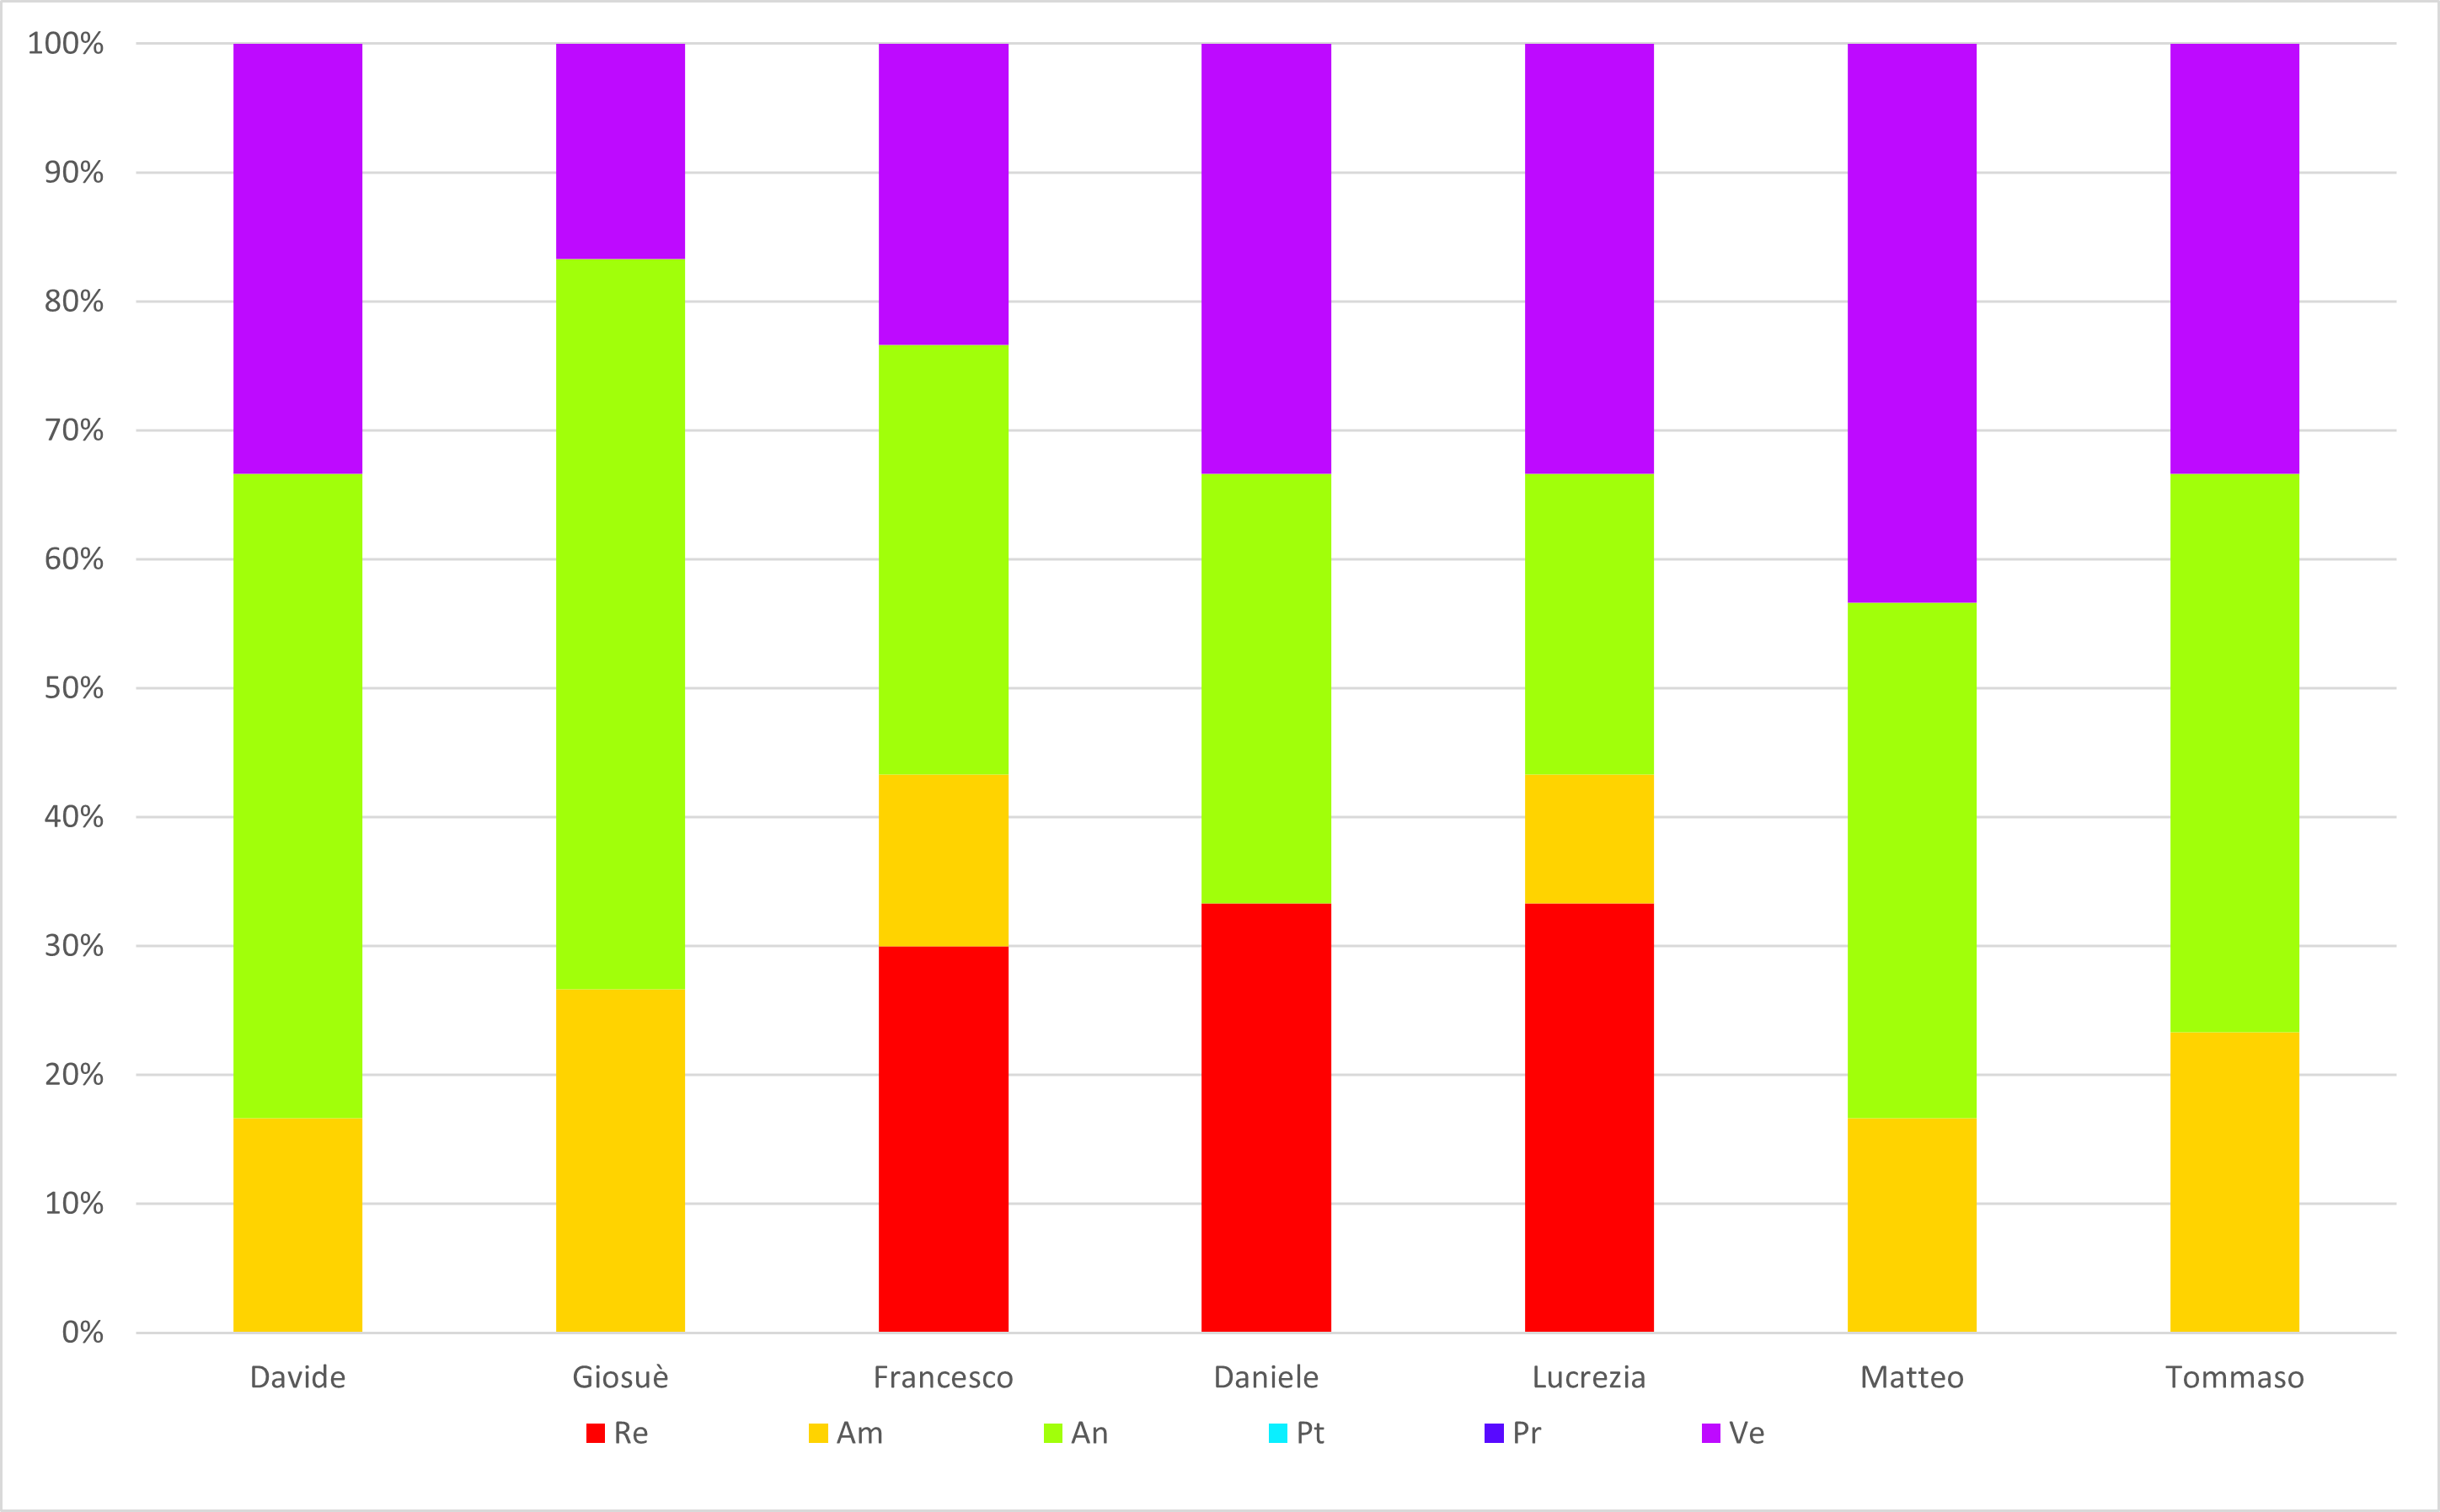
\includegraphics[scale = 0.5]{components/img/Analisi-isto.png}
    \caption{ Istogramma della ripartizione di ore per ruolo in Analisi}
    \label{fig:istogramma ripartizione ore , fase di Analisi}
\end{figure}
\subsubsection{Prospetto economico}
Il costo per ogni ruolo è il seguente:
\begin{table}[H]
		\begin{center}
			\setlength{\aboverulesep}{0pt}
			\setlength{\belowrulesep}{0pt}
			\setlength{\extrarowheight}{.75ex}
			\rowcolors{2}{AzzurroGruppo!10}{white}
			\begin{tabular}{ c c c }
				\rowcolor{AzzurroGruppo!30} 
				\textbf{Ruolo} & \textbf{Ore} & \textbf{Costo}  \\
				\toprule
				Responsabile & 29 & 870 \euro \\
				Amministratore & 32 & 640 \euro \\
				Analista & 84 & 2100 \euro \\
				Progettista & - & - \\
				Programmatore & - & - \\
				Verificatore & 65 & 975 \euro \\
				\textbf{Totale} & \textbf{210} & \textbf{4585 \euro} \\
				\bottomrule
			\end{tabular}
			\caption{ Prospetto dei costi per ruoli nel periodo di Analisi}
		\end{center}
\end{table}
I dati ottenuti si possono riassumere nel seguente areogramma:
\begin{figure}[H]
    \centering
    \includegraphics[scale = 0.5]{components/img/analisi-torta.png}
    \caption{ Areogramma ripartizione ore , fase di Analisi}
    \label{fig:Areogramma ripartizione ore , fase di Analisi}
\end{figure}
\subsection{Fase di consolidamento dei requisiti}
\subsubsection{Prospetto orario}
Durante il periodo di consolidamento dei \glo{requisiti} viene effettuata la seguente distribuzione oraria:
\begin{table}[H]
		\begin{center}
			\setlength{\aboverulesep}{0pt}
			\setlength{\belowrulesep}{0pt}
			\setlength{\extrarowheight}{.75ex}
			\rowcolors{2}{AzzurroGruppo!10}{white}
			\begin{tabular}{ c c c c c c c c }
				\rowcolor{AzzurroGruppo!30} 
				\textbf{Nominativo} & \textbf{Re} & \textbf{Am} & \textbf{An} & \textbf{Pt} & \textbf{Pr} & \textbf{Ve} & \textbf{Ore Totali}  \\
				\toprule
				\Davide    & - & - & 3 & - & - & 2 & 5 \\
				\Giosue    & - & - & - & - & - & 5 & 5 \\
				\Francesco & - & - & 5 & - & - & - & 5\\
				\Daniele   & - & 3 & - & - & - & 2 & 5\\
				\Lucrezia  & 3 & - & - & - & - & 2 & 5\\
				\Matteo    & - & - & 5 & - & - & - & 5\\
				\Tommaso    & - & - & 3 & - & - & 2 & 5\\
				 \textbf{Ore totali} & \textbf{3} & \textbf{3} & \textbf{16} & \textbf{-} & \textbf{-} & \textbf{13} & \textbf{35} \\
				\bottomrule
			\end{tabular}
			\caption{Distribuzione delle ore nel periodo di Consolidamento dei requisiti}
		\end{center}
	\end{table}
I dati ottenuti vengono riassunti nel seguente istogramma:
\begin{figure}[H]
    \centering
    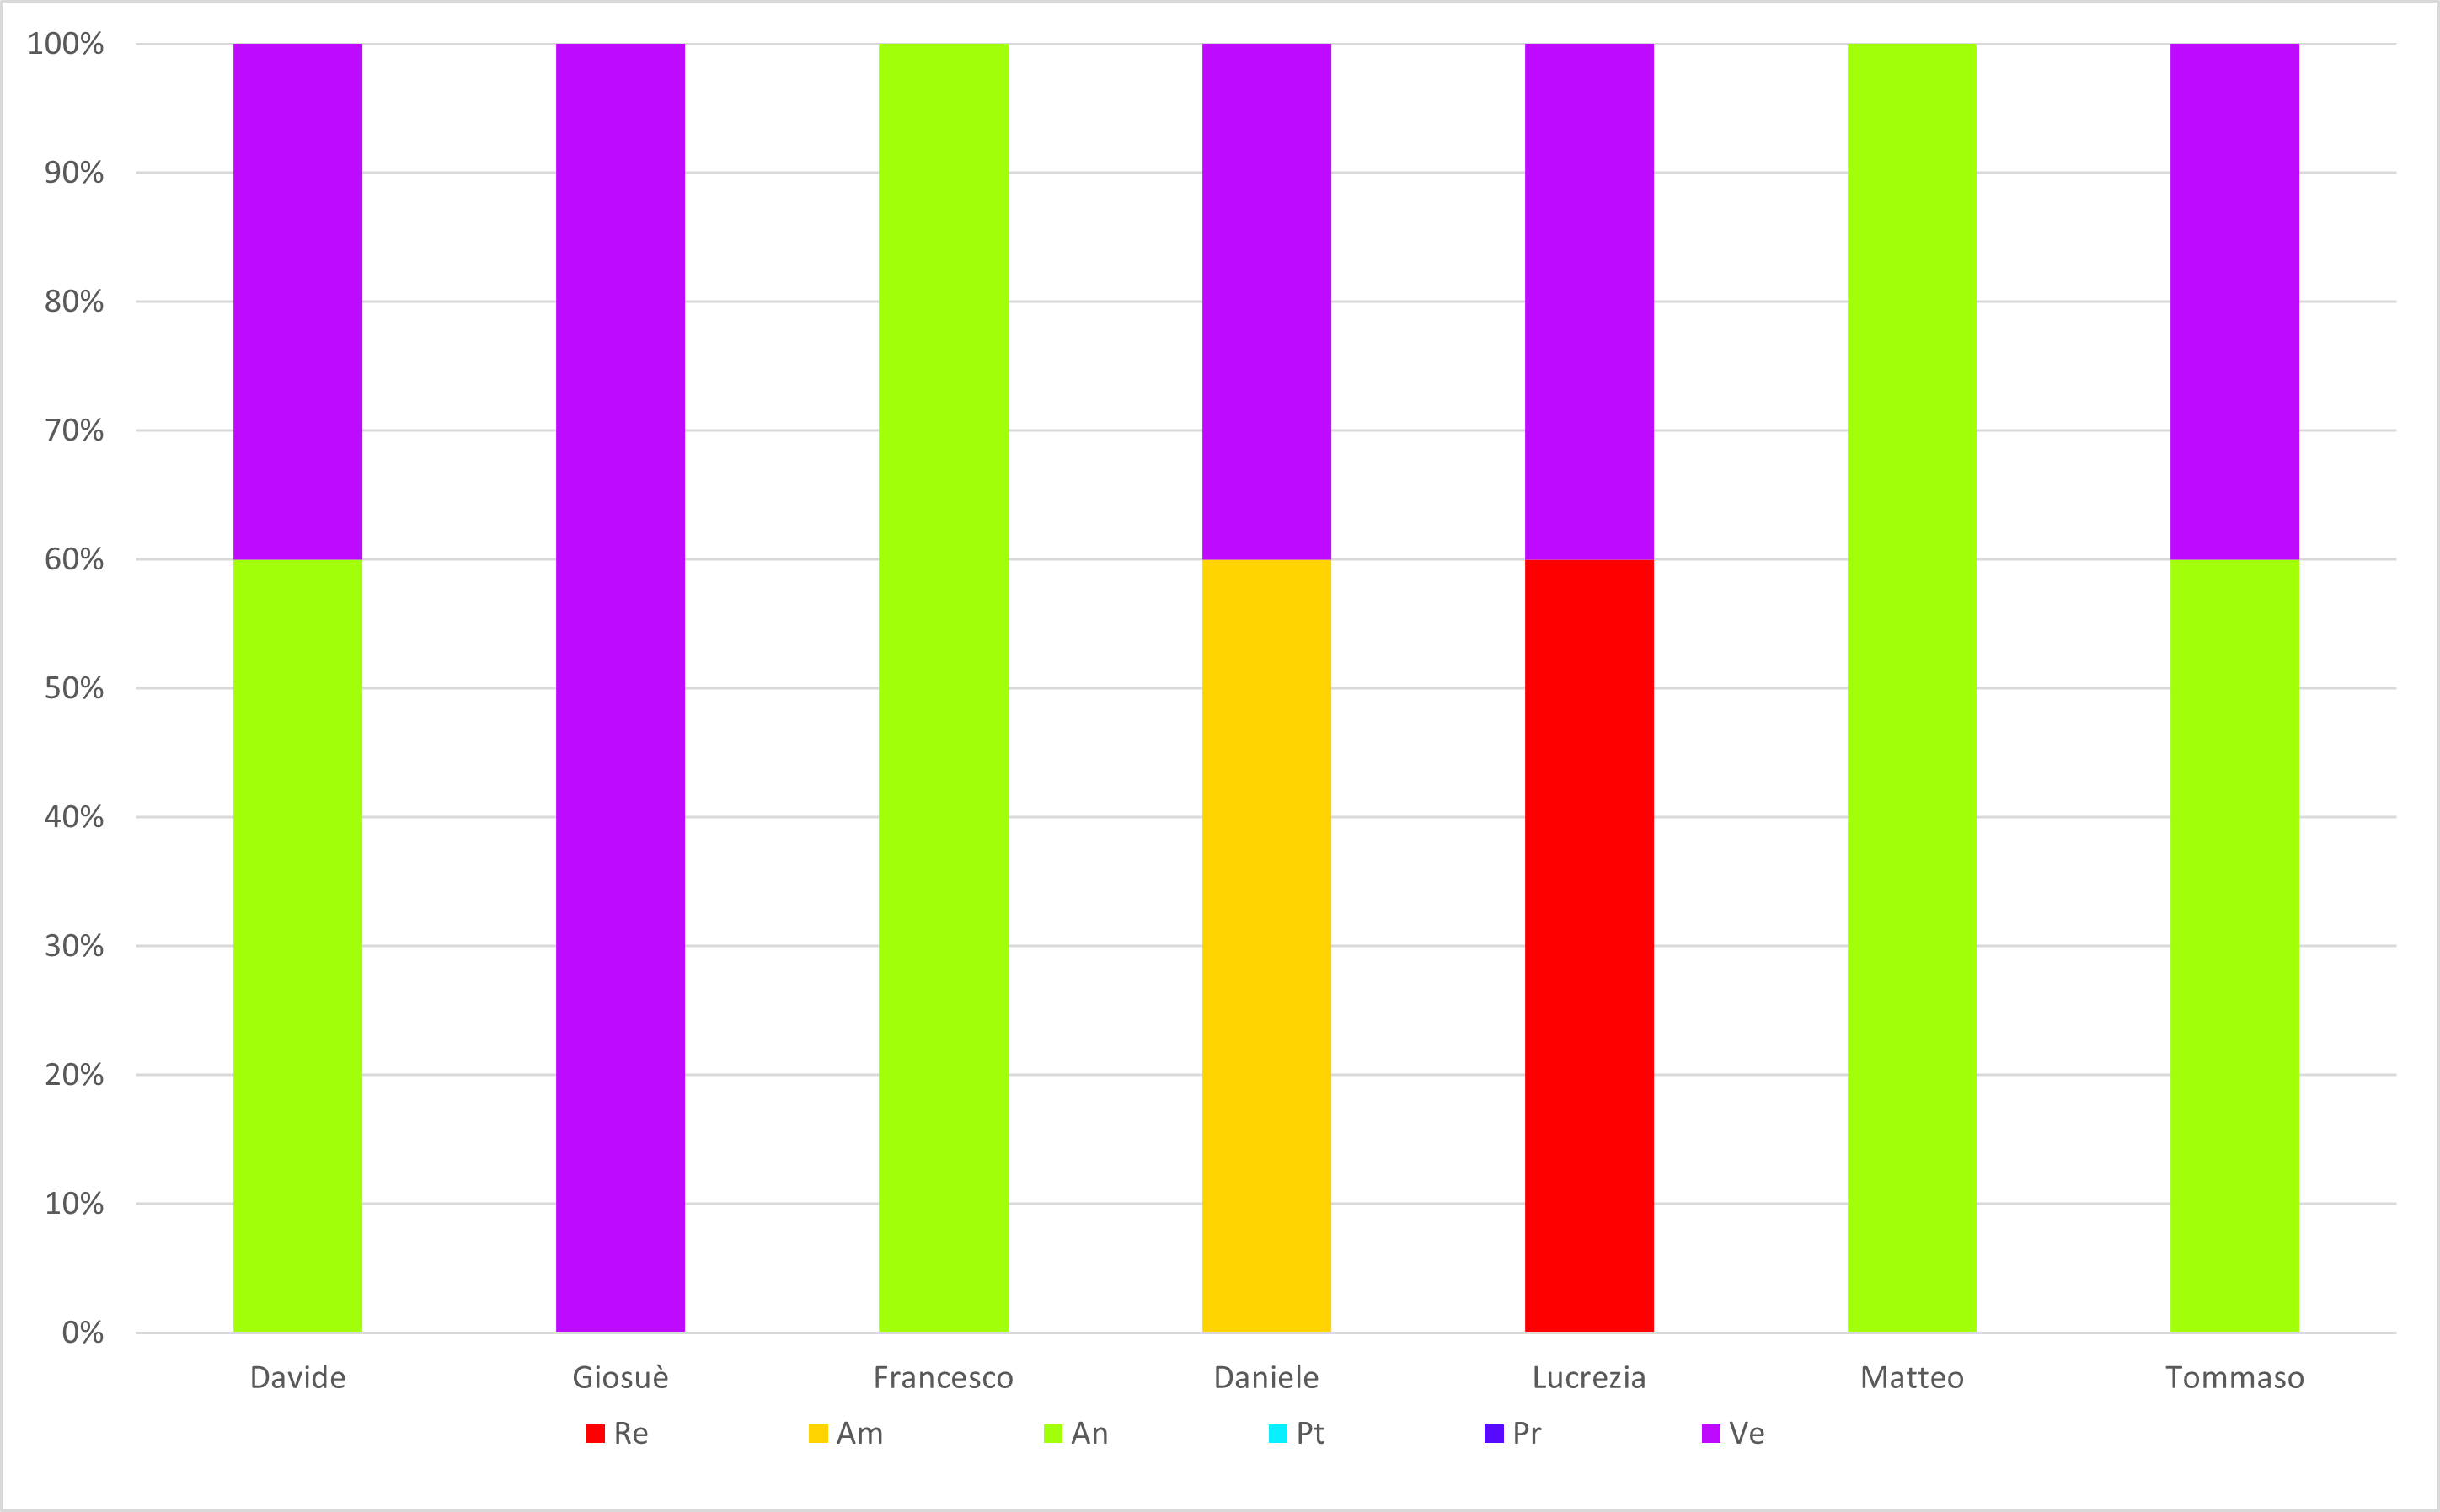
\includegraphics[scale = 0.5]{components/img/Analisi-consolidamento-isto.png}
    \caption{Istogramma della ripartizione di ore per ruolo in Consolidamento dei requisiti}
    \label{fig:istogramma ripartizione ore , fase di Consolidamento dei Requisiti}
\end{figure}
\subsubsection{Prospetto economico}
Il costo per ogni ruolo è il seguente:
\begin{table}[H]
		\begin{center}
			\setlength{\aboverulesep}{0pt}
			\setlength{\belowrulesep}{0pt}
			\setlength{\extrarowheight}{.75ex}
			\rowcolors{2}{AzzurroGruppo!10}{white}
			\begin{tabular}{ c c c }
				\rowcolor{AzzurroGruppo!30} 
				\textbf{Ruolo} & \textbf{Ore} & \textbf{Costo}  \\
				\toprule
				Responsabile   & 3 & 90 \euro \\
				Amministratore & 3 & 60 \euro \\
				Analista       & 16 & 400 \euro \\
				Progettista    & - & - \\
				Programmatore  & - & - \\
				Verificatore   & 13 & 195 \euro \\
				\textbf{Totale} & \textbf{35} & \textbf{745 \euro} \\
				\bottomrule
			\end{tabular}
			\caption{ Prospetto dei costi per ruoli nel periodo di Consolidamento dei requisiti}
		\end{center}
	\end{table}
I dati ottenuti si possono riassumere nel seguente areogramma:
\begin{figure}[H]
    \centering
    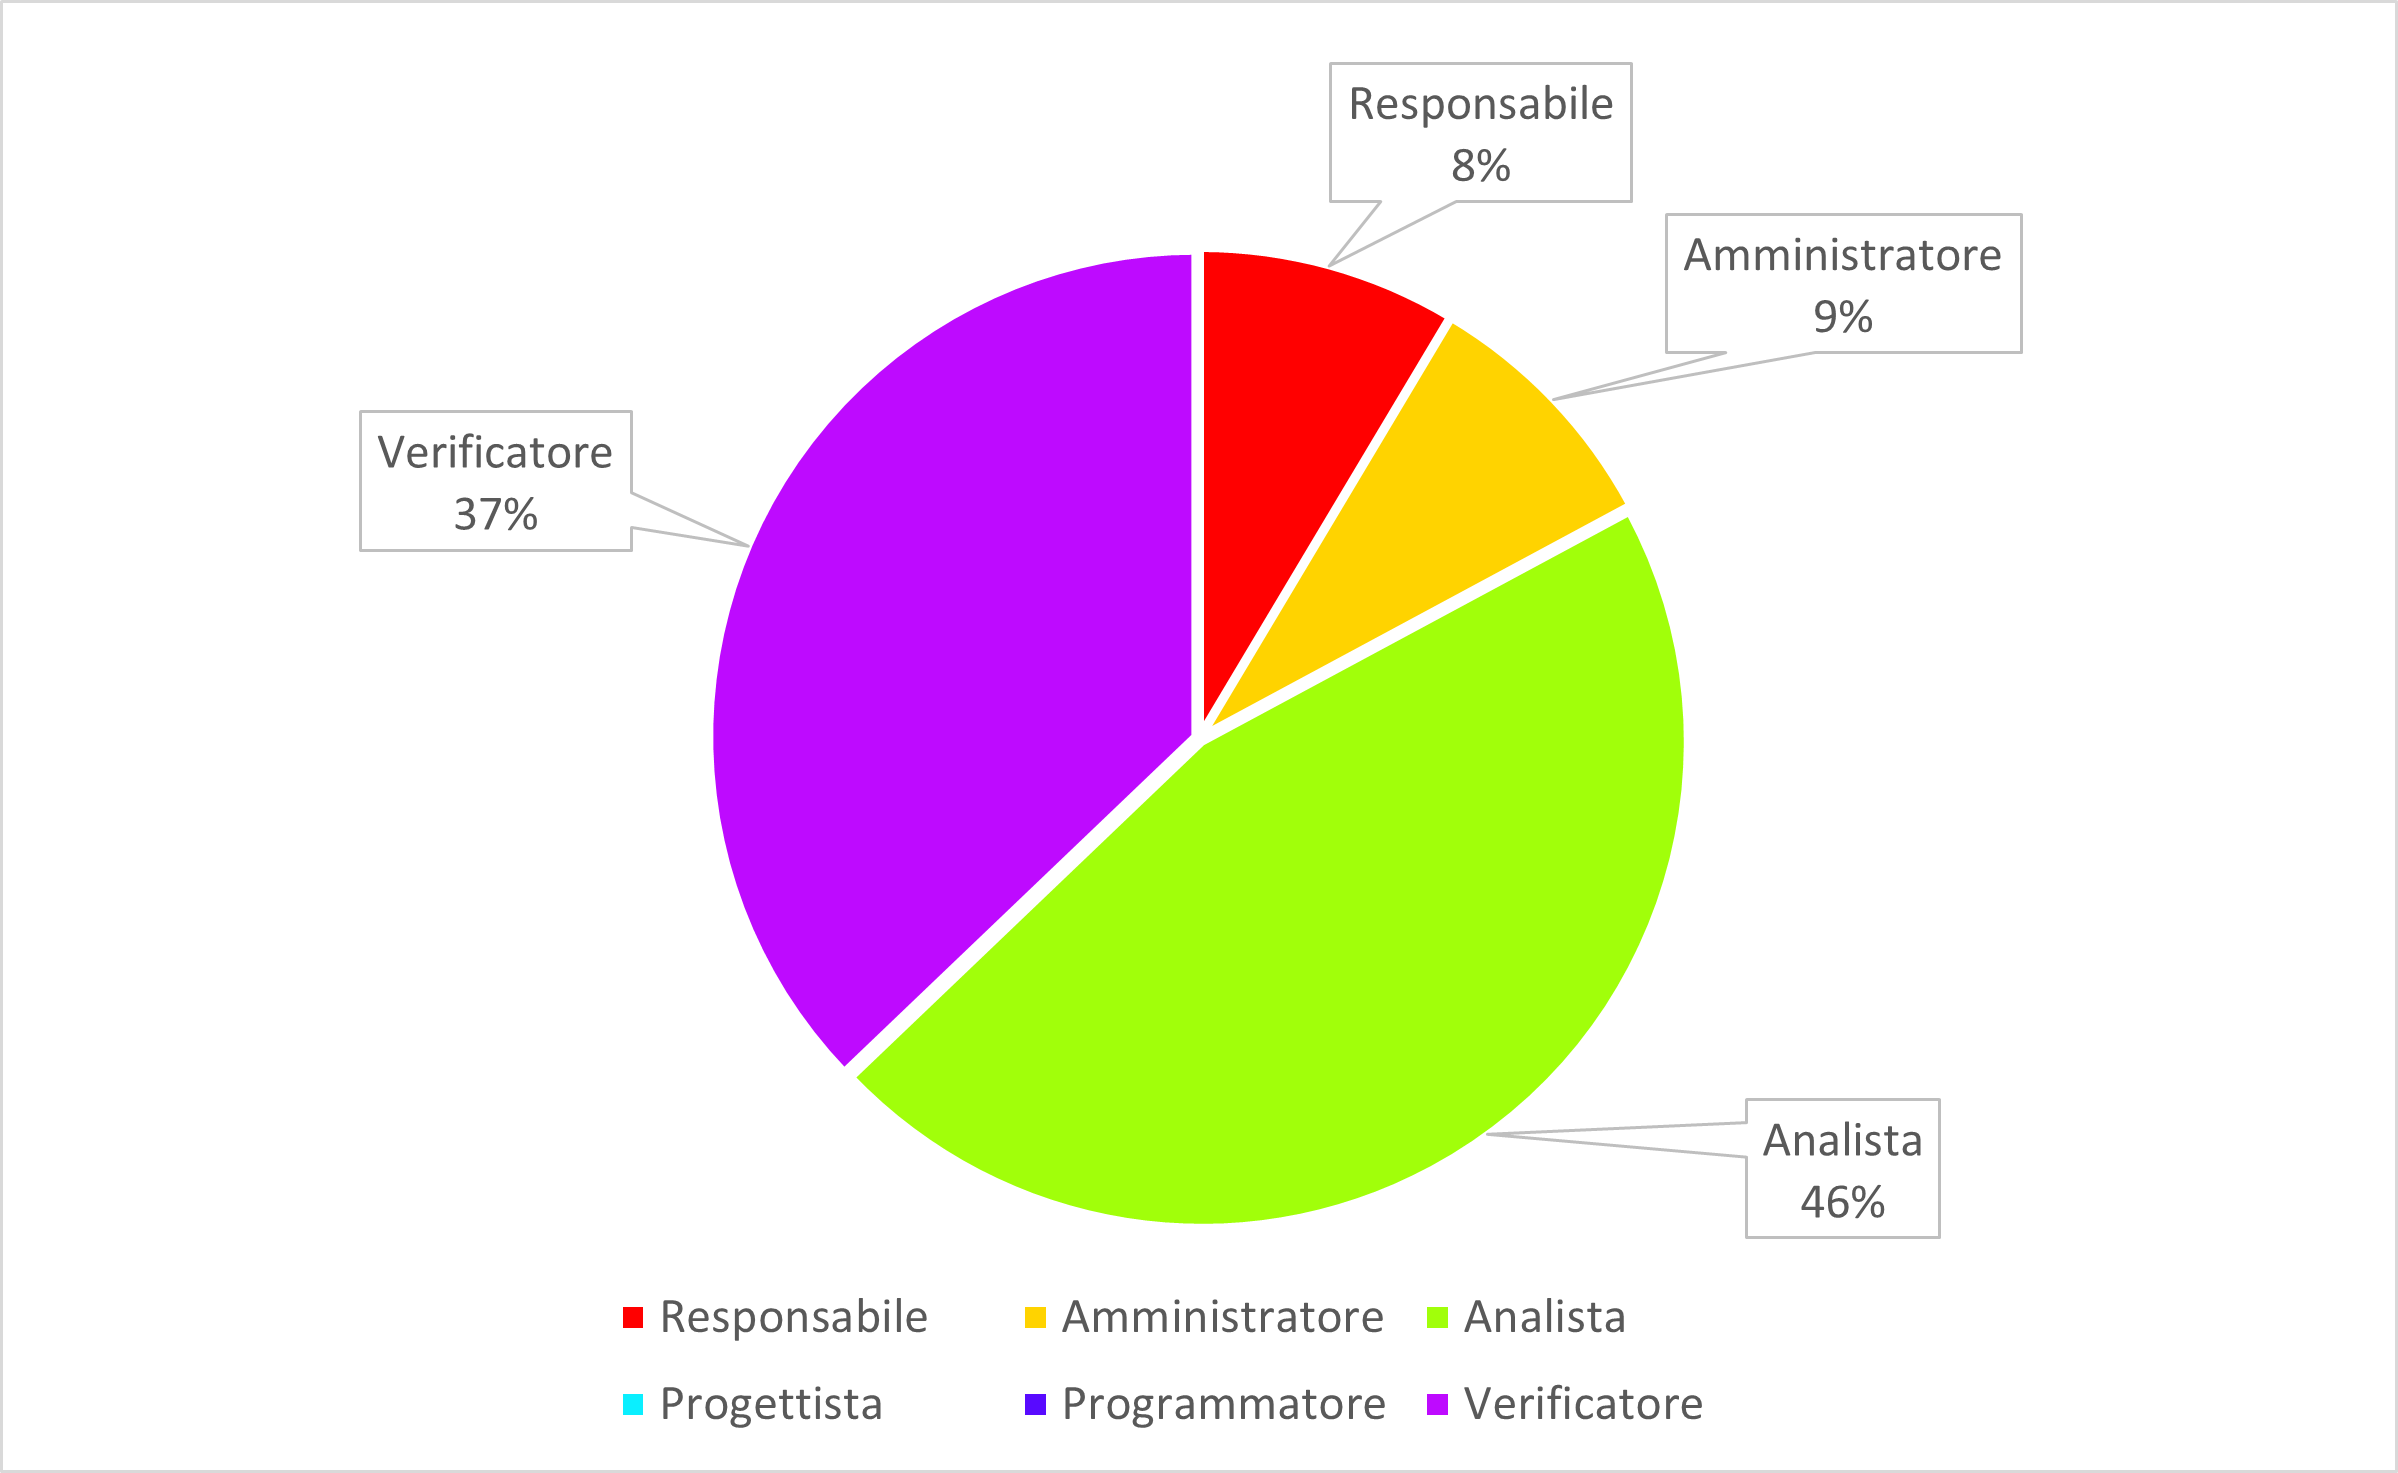
\includegraphics[scale = 0.5]{components/img/Analisi-consolidamento-torta.png}
    \caption{ Areogramma della ripartizione di ore per ruolo in Consolidamento dei Requisiti}
    \label{fig:Areogramma ripartizione ore , fase di Consolidamento dei requisiti}
\end{figure}
\subsection{Fase di Progettazione architetturale}
\subsubsection{Prospetto orario}
In questa fase la distribuzione oraria è la seguente:
\begin{table}[H]
		\begin{center}
			\setlength{\aboverulesep}{0pt}
			\setlength{\belowrulesep}{0pt}
			\setlength{\extrarowheight}{.75ex}
			\rowcolors{2}{AzzurroGruppo!10}{white}
			\begin{tabular}{ c c c c c c c c }
				\rowcolor{AzzurroGruppo!30} 
				\textbf{Nominativo} & \textbf{Re} & \textbf{Am} & \textbf{An} & \textbf{Pt} & \textbf{Pr} & \textbf{Ve} & \textbf{Ore Totali}  \\
				\toprule
				\Davide    & 5  & 6 & -  & -  & 4 & 15 & 30 \\
				\Giosue    & 3  & - & -  & 16 & 5 & 6  & 30 \\
				\Francesco & -  & - & 8  & 12 & 3 & 7  & 30\\
				\Daniele   & -  & 3 & 10 & 13 & - & 4  & 30\\
				\Lucrezia  & -  & - & 10 & -  & 4 & 16 & 30\\
				\Matteo    & 10 & 8 & -  & 12 & - & -  & 30\\
				\Tommaso   & -  & 3 & 10 & 8  & 5 & 4  & 30\\
				 \textbf{Ore totali} & \textbf{18} & \textbf{20} & \textbf{38} & \textbf{61} & \textbf{21} & \textbf{52} & \textbf{210} \\
				\bottomrule
			\end{tabular}
			\caption{Distribuzione delle ore nel periodo di  Progettazione architetturale}
		\end{center}
	\end{table}
I dati ottenuti vengono riassunti nel seguente istogramma:
\begin{figure}[H]
    \centering
    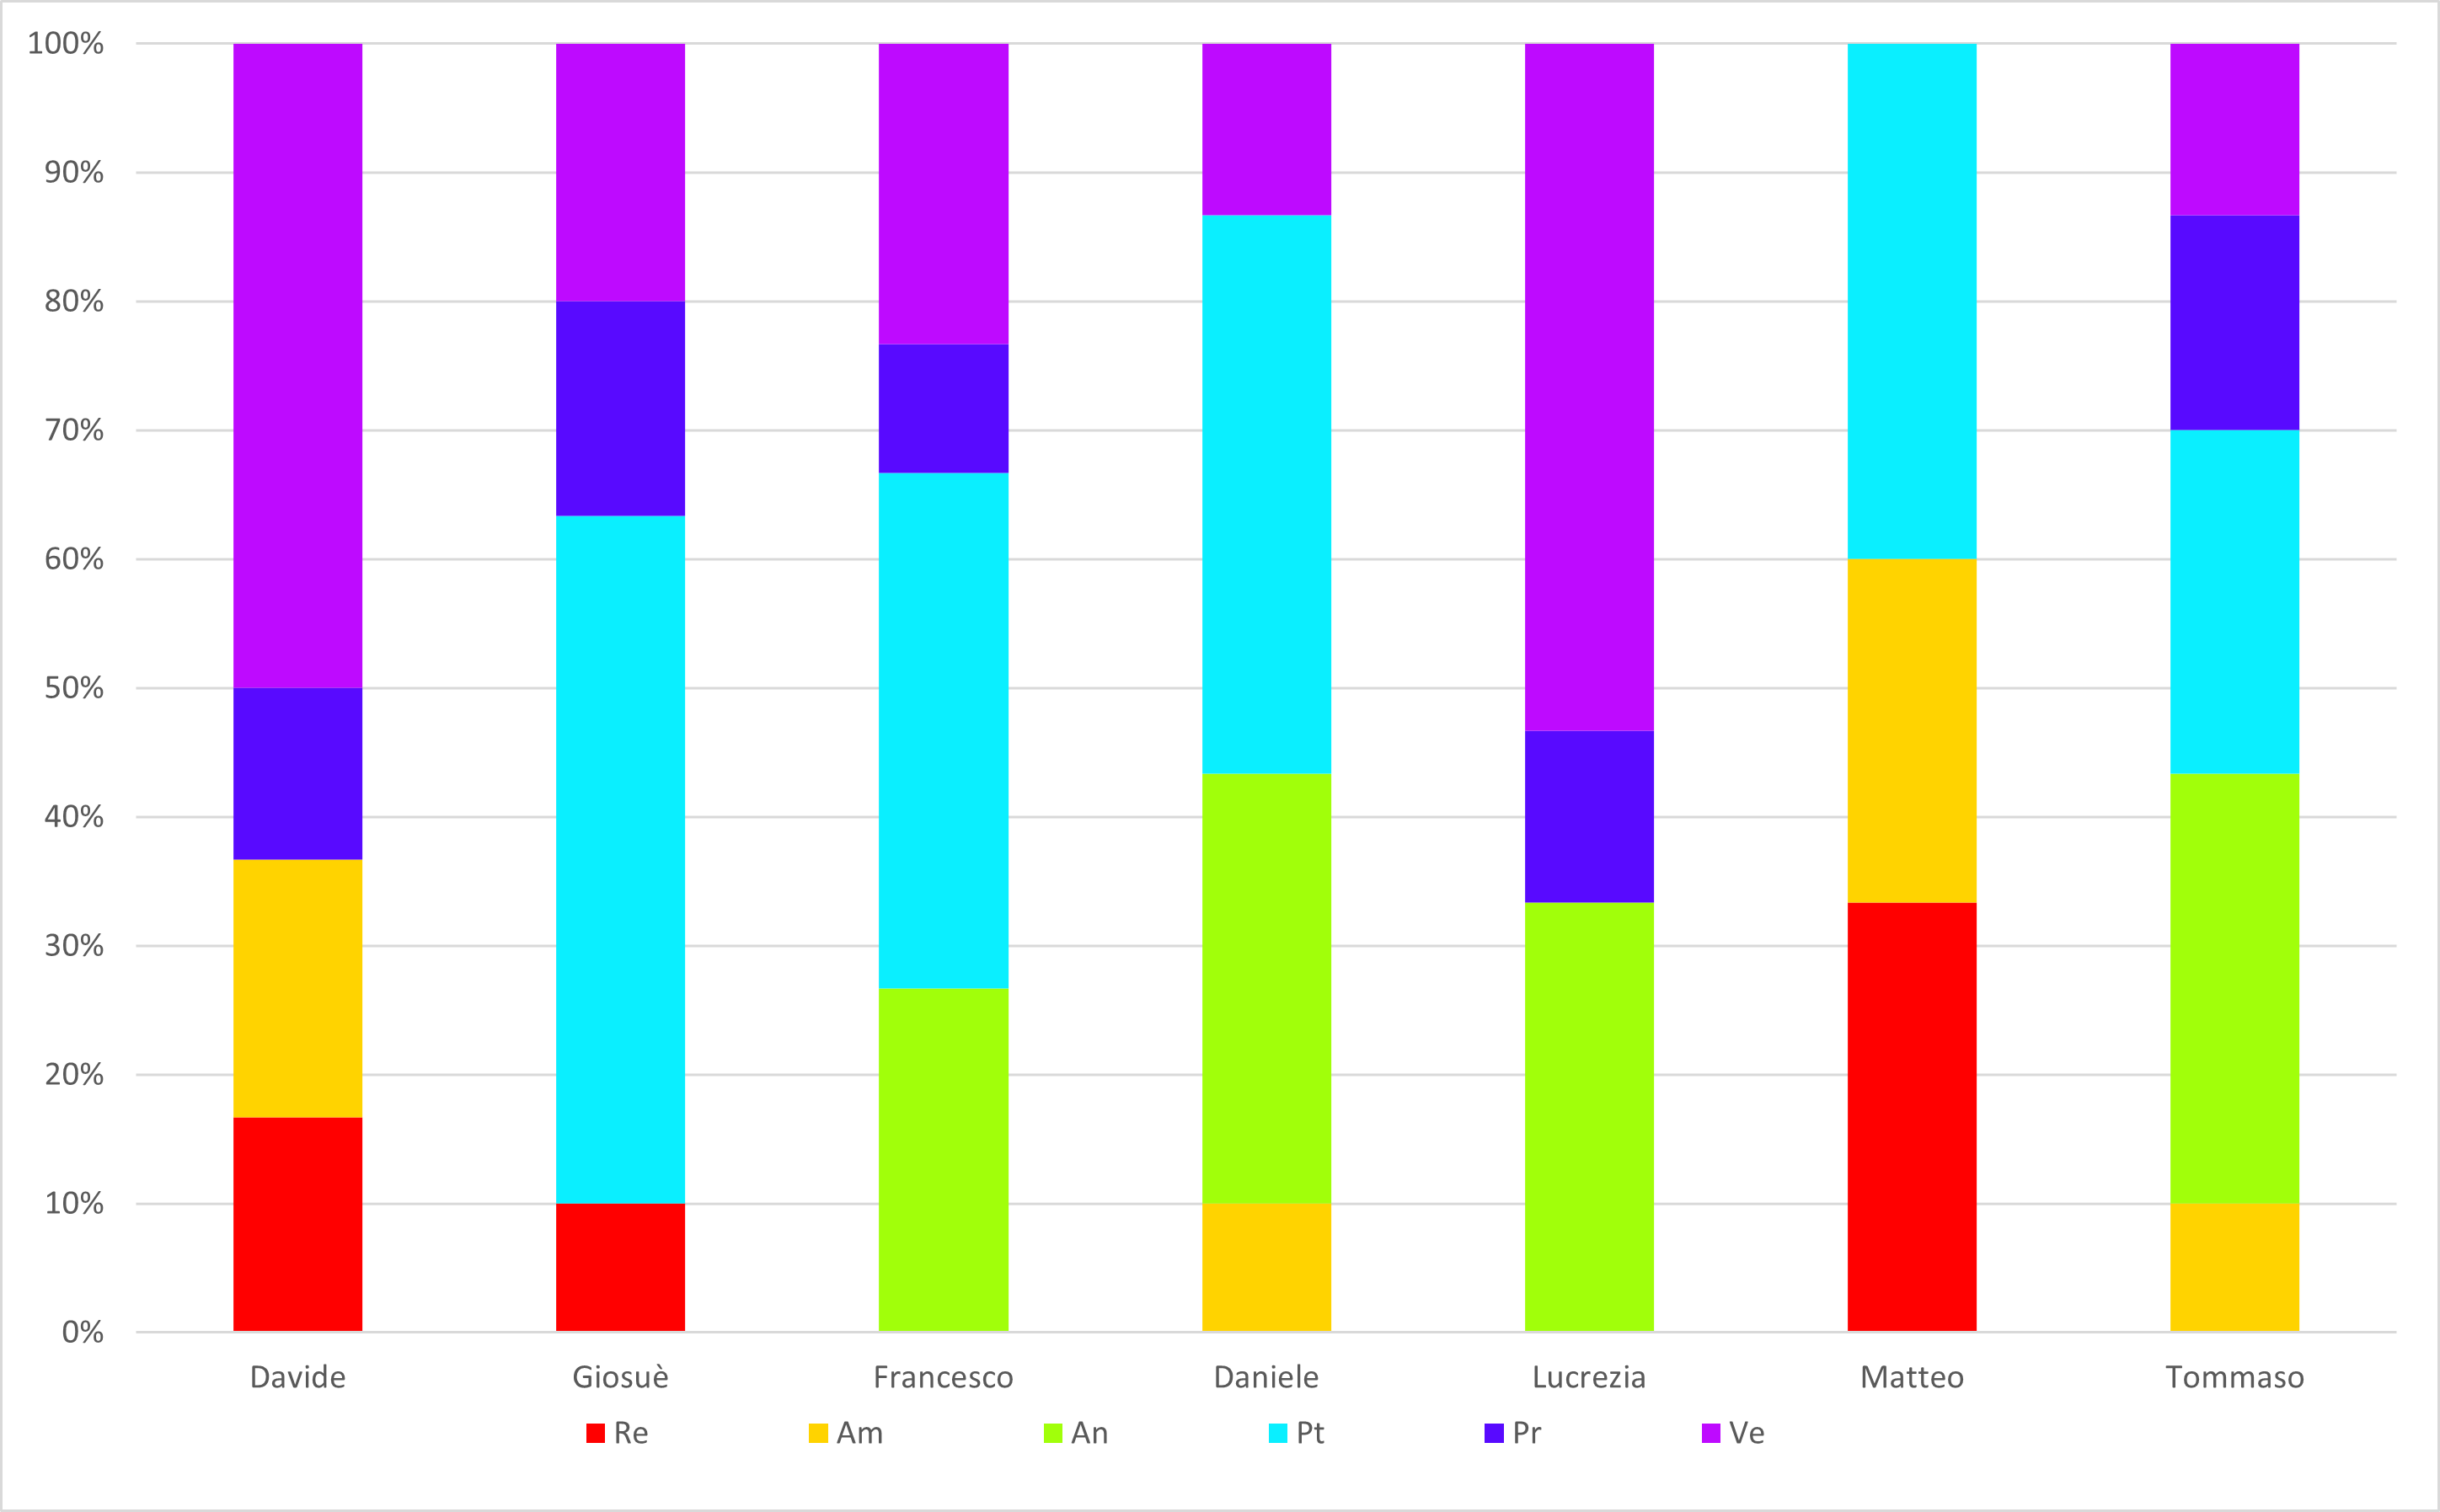
\includegraphics[scale = 0.5]{components/img/Architettura-isto.png}
    \caption{Istogramma della ripartizione di ore per ruolo in Progettazione architetturale}
    \label{fig:istogramma ripartizione ore , fase di Progettazione architetturale}
\end{figure}
\subsubsection{Prospetto economico}
Il costo per ogni ruolo è il seguente:
\begin{table}[H]
		\begin{center}
			\setlength{\aboverulesep}{0pt}
			\setlength{\belowrulesep}{0pt}
			\setlength{\extrarowheight}{.75ex}
			\rowcolors{2}{AzzurroGruppo!10}{white}
			\begin{tabular}{ c c c }
				\rowcolor{AzzurroGruppo!30} 
				\textbf{Ruolo} & \textbf{Ore} & \textbf{Costo} \\
				\toprule
				Responsabile   & 18 & 540 \euro \\
				Amministratore & 20 & 400 \euro \\
				Analista       & 38 & 950 \euro \\
				Progettista    & 61 & 1342 \euro \\
				Programmatore  & 21 & 315 \euro \\
				Verificatore   & 52 & 780 \euro \\
				\textbf{Totale} & \textbf{210} & \textbf{4327 \euro} \\
				\bottomrule
			\end{tabular}
			\caption{ Prospetto dei costi per ruoli nel periodo di Progettazione architetturale}
		\end{center}
	\end{table}
I dati ottenuti si possono riassumere nel seguente areogramma:
\begin{figure}[H]
    \centering
    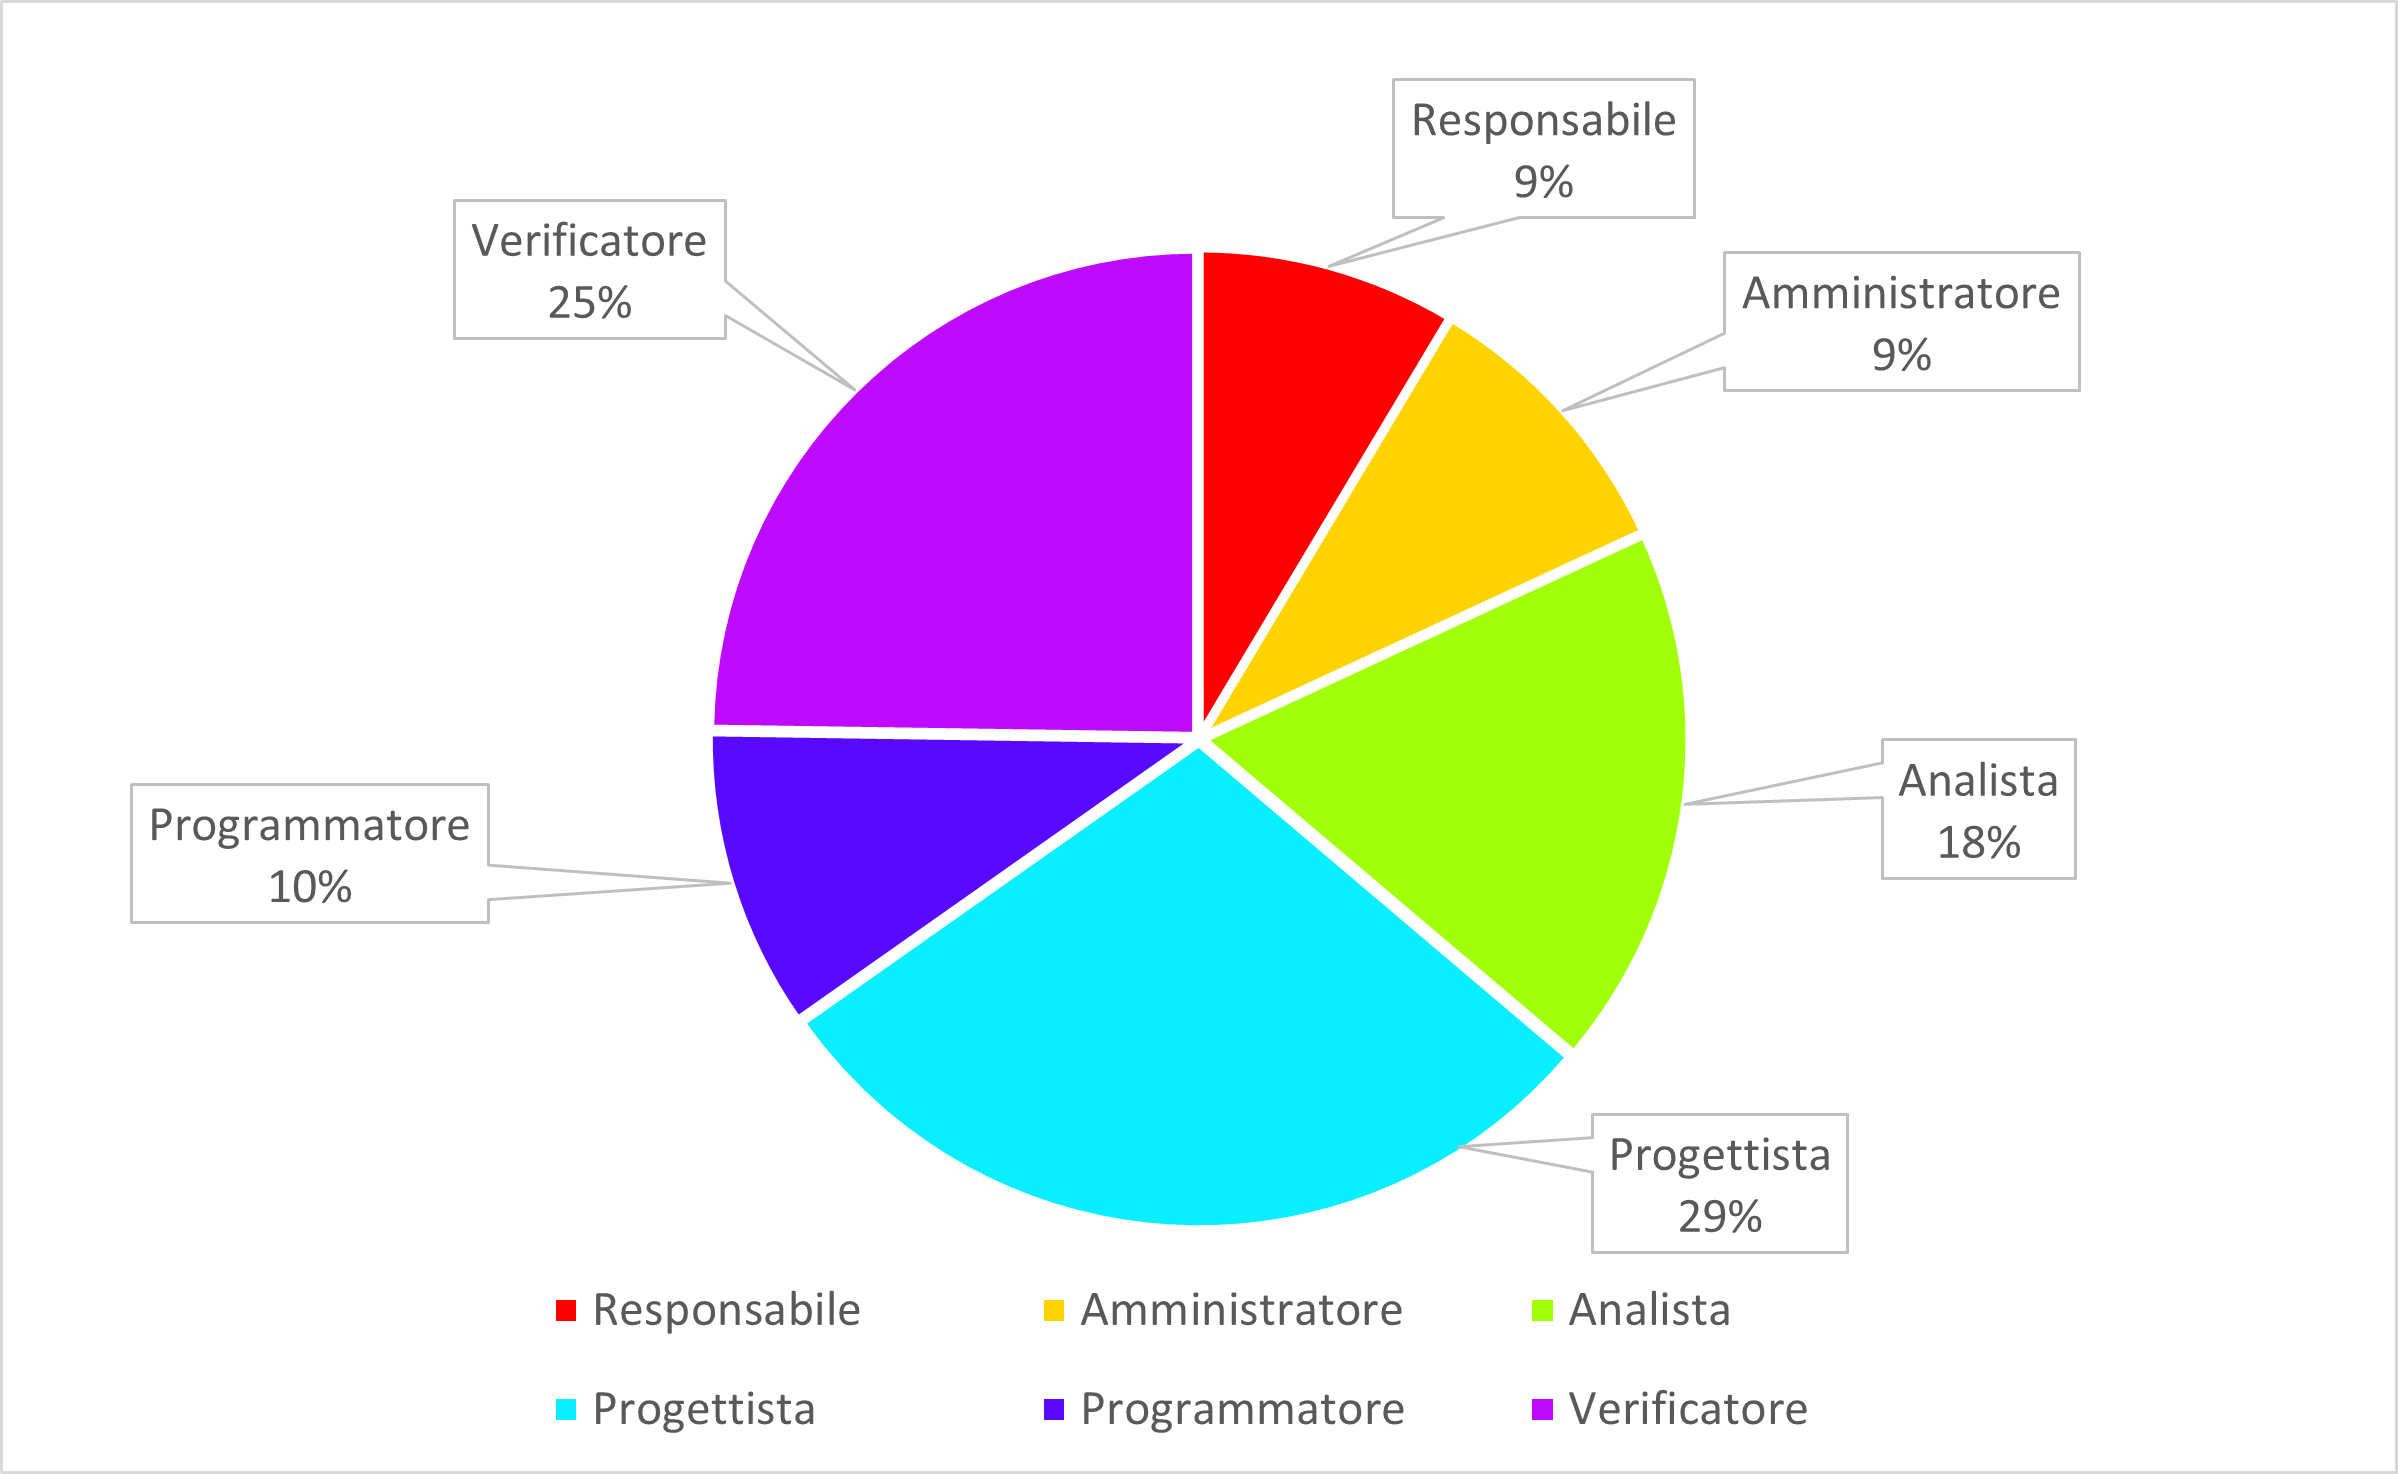
\includegraphics[scale = 0.5]{components/img/Architettura-torta.png}
    \caption{ Areogramma della ripartizione di ore per ruolo in Progettazione architetturale}
    \label{fig:Areogramma ripartizione ore , fase di Progettazione architetturale}
\end{figure}
\subsection{Fase di Progettazione di dettaglio e codifica}

\subsubsection{Sprint 8}

In questo sprint la distribuzione oraria è la seguente:
\begin{table}[H]
		\begin{center}
			\setlength{\aboverulesep}{0pt}
			\setlength{\belowrulesep}{0pt}
			\setlength{\extrarowheight}{.75ex}
			\rowcolors{2}{AzzurroGruppo!10}{white}
			\begin{tabular}{ c c c c c c c c }
				\rowcolor{AzzurroGruppo!30} 
				\textbf{Nominativo} & \textbf{Re} & \textbf{Am} & \textbf{An} & \textbf{Pt} & \textbf{Pr} & \textbf{Ve} & \textbf{Ore Totali}  \\
				\toprule
				\Davide    & - & - & - & 8 & 10 & 7 & 25 \\
				\Giosue    & 4 & 2 & - & 3 & 11 & 5 & 25 \\
				\Francesco & 4 & 4 & - & 6 & 6 & 5 & 25 \\
				\Daniele   & - & - & - & 7 & 10 & 8 & 25 \\
				\Lucrezia  & - & 4 & - & 7 & 8 & 6 & 25 \\
				\Matteo    & - & - & - & 7 & 13 & 5 & 25 \\
				\Tommaso   & - & - & - & 6 & 13 & 6 & 25 \\
				 \textbf{Ore totali} & \textbf{8} & \textbf{10} & \textbf{-} & \textbf{44} & \textbf{71} & \textbf{42} & \textbf{175} \\
				\bottomrule
			\end{tabular}
			\caption{Distribuzione delle ore nello sprint 8}
		\end{center}
	\end{table}


\subsubsection{Sprint 9}

In questo sprint la distribuzione oraria è la seguente:
\begin{table}[H]
		\begin{center}
			\setlength{\aboverulesep}{0pt}
			\setlength{\belowrulesep}{0pt}
			\setlength{\extrarowheight}{.75ex}
			\rowcolors{2}{AzzurroGruppo!10}{white}
			\begin{tabular}{ c c c c c c c c }
				\rowcolor{AzzurroGruppo!30} 
				\textbf{Nominativo} & \textbf{Re} & \textbf{Am} & \textbf{An} & \textbf{Pt} & \textbf{Pr} & \textbf{Ve} & \textbf{Ore Totali}  \\
				\toprule
				\Davide    & - & - & - & 7 & 10 & 8 & 25 \\
				\Giosue    & - & - & - & 3 & 10 & 12 & 25 \\
				\Francesco & - & - & - & 6 & 14 & 5 & 25 \\
				\Daniele   & - & - & 2 & 8 & 8 & 7 & 25 \\
				\Lucrezia  & - & 4 & - & 8 & 7 & 6 & 25 \\
				\Matteo    & 4 & - & - & 8 & 8 & 5 & 25 \\
				\Tommaso   & 4 & 4 & - & 5 & 6 & 6 & 25 \\
				 \textbf{Ore totali} & \textbf{8} & \textbf{8} & \textbf{2} & \textbf{45} & \textbf{63} & \textbf{49} & \textbf{175} \\
				\bottomrule
			\end{tabular}
			\caption{Distribuzione delle ore nello sprint 9}
		\end{center}
	\end{table}


\subsubsection{Prospetto orario}
In questa fase la distribuzione oraria è la seguente:
\begin{table}[H]
		\begin{center}
			\setlength{\aboverulesep}{0pt}
			\setlength{\belowrulesep}{0pt}
			\setlength{\extrarowheight}{.75ex}
			\rowcolors{2}{AzzurroGruppo!10}{white}
			\begin{tabular}{ c c c c c c c c }
				\rowcolor{AzzurroGruppo!30} 
				\textbf{Nominativo} & \textbf{Re} & \textbf{Am} & \textbf{An} & \textbf{Pt} & \textbf{Pr} & \textbf{Ve} & \textbf{Ore Totali}  \\
				\toprule
				\Davide    & - & - & - & 15 & 20 & 15 & 50 \\
				\Giosue    & 4 & 2 & - & 6 & 21 & 17 & 50 \\
				\Francesco & 4 & 4 & - & 12 & 20 & 10 & 50 \\
				\Daniele   & - & - & 2 & 15 & 18 & 15 & 50 \\
				\Lucrezia  & - & 8 & - & 15 & 15 & 12 & 50 \\
				\Matteo    & 4 & - & - & 15 & 21 & 10 & 50 \\
				\Tommaso   & 4 & 4 & - & 11 & 19 & 12 & 50 \\
				 \textbf{Ore totali} & \textbf{16} & \textbf{18} & \textbf{2} & \textbf{89} & \textbf{134} & \textbf{91} & \textbf{350} \\
				\bottomrule
			\end{tabular}
			\caption{Distribuzione delle ore nel periodo di Progettazione di dettaglio e codifica}
		\end{center}
	\end{table}
	I dati ottenuti vengono riassunti nel seguente istogramma:
\begin{figure}[H]
    \centering
    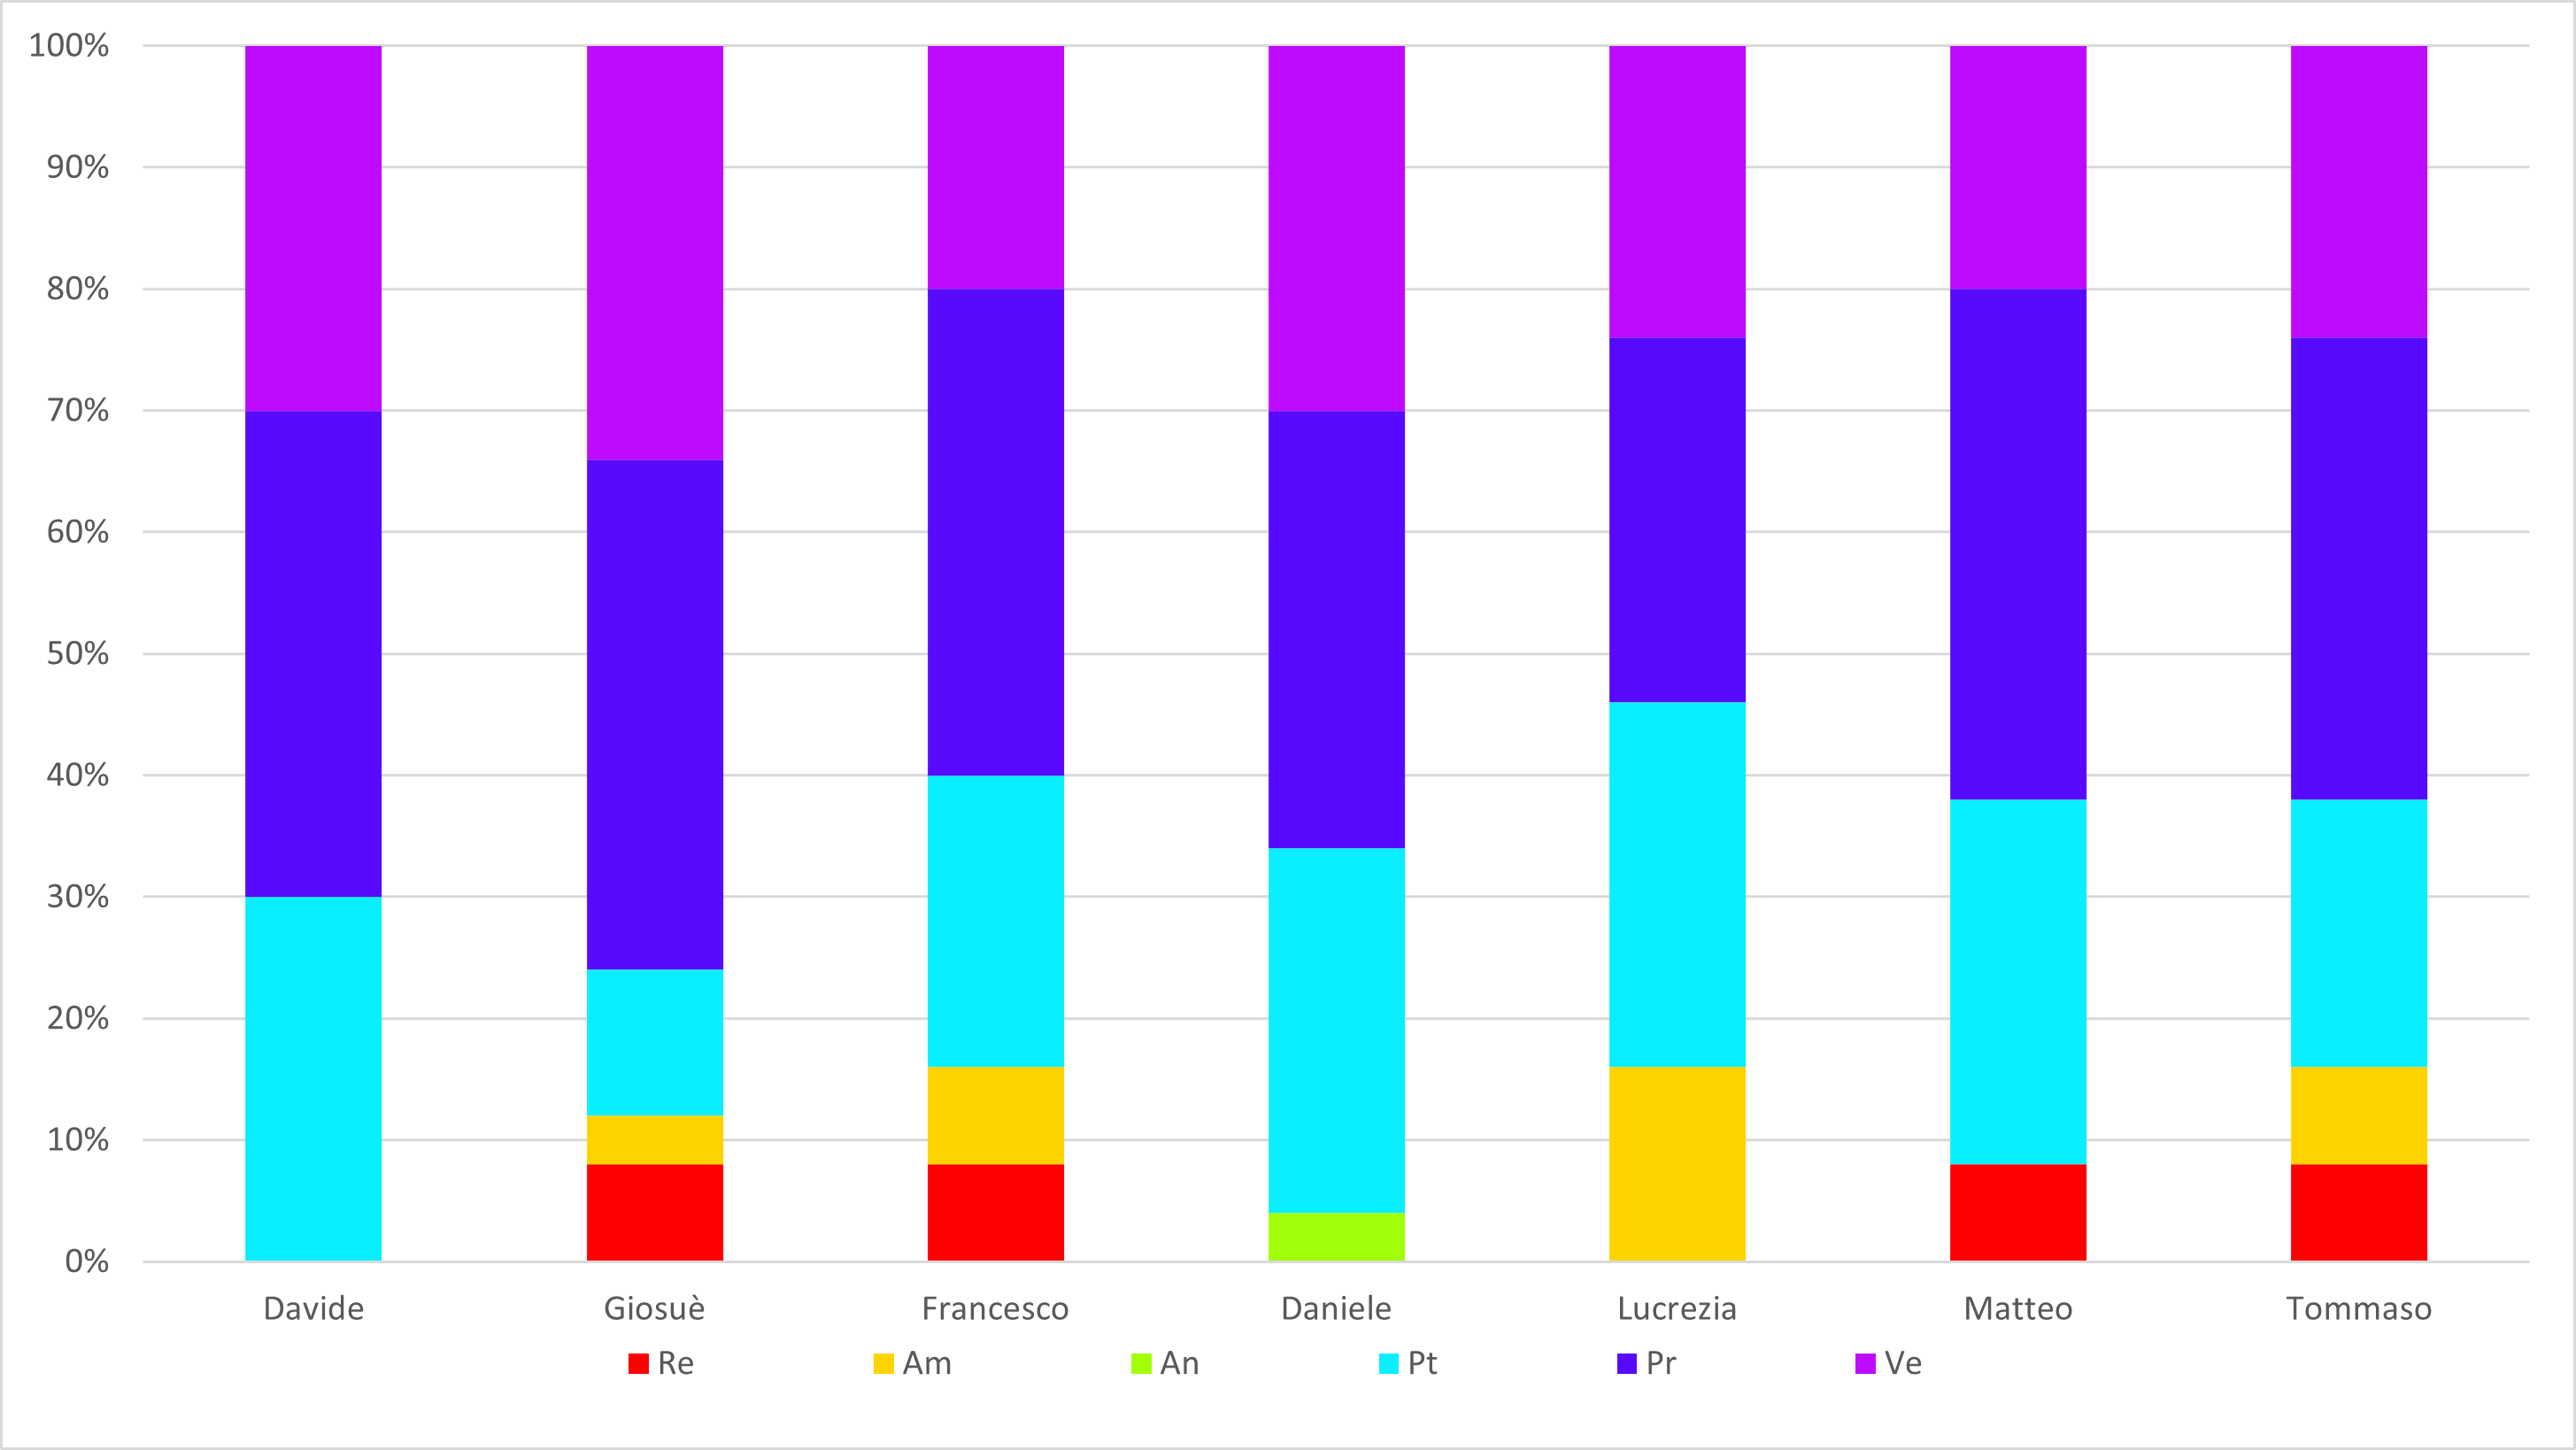
\includegraphics[scale = 0.5]{components/img/Sprint-8-9-isto.png}
    \caption{Istogramma della ripartizione di ore per ruolo in Progettazione di dettaglio e codifica}
    \label{fig:istogramma ripartizione ore , fase di Progettazione di dettaglio e codifica}
\end{figure}
\subsubsection{Prospetto economico}
Il costo per ogni ruolo è il seguente:
\begin{table}[H]
		\begin{center}
			\setlength{\aboverulesep}{0pt}
			\setlength{\belowrulesep}{0pt}
			\setlength{\extrarowheight}{.75ex}
			\rowcolors{2}{AzzurroGruppo!10}{white}
			\begin{tabular}{ c c c }
				\rowcolor{AzzurroGruppo!30} 
				\textbf{Ruolo} & \textbf{Ore} & \textbf{Costo}  \\
				\toprule
				Responsabile   & 16 & 480 \euro \\
				Amministratore & 18 & 360 \euro \\
				Analista       & 2 & 50 \euro \\
				Progettista    & 89 & 1958 \euro \\
				Programmatore  & 134 & 2010 \euro \\
				Verificatore   & 91 & 1365 \euro \\
				\textbf{Totale} & \textbf{350} & \textbf{6223 \euro} \\
				\bottomrule
			\end{tabular}
			\caption{ Prospetto dei costi per ruoli nel periodo di Progettazione di dettaglio e codifica}
		\end{center}
	\end{table}
I dati ottenuti si possono riassumere nel seguente areogramma:
\begin{figure}[H]
    \centering
    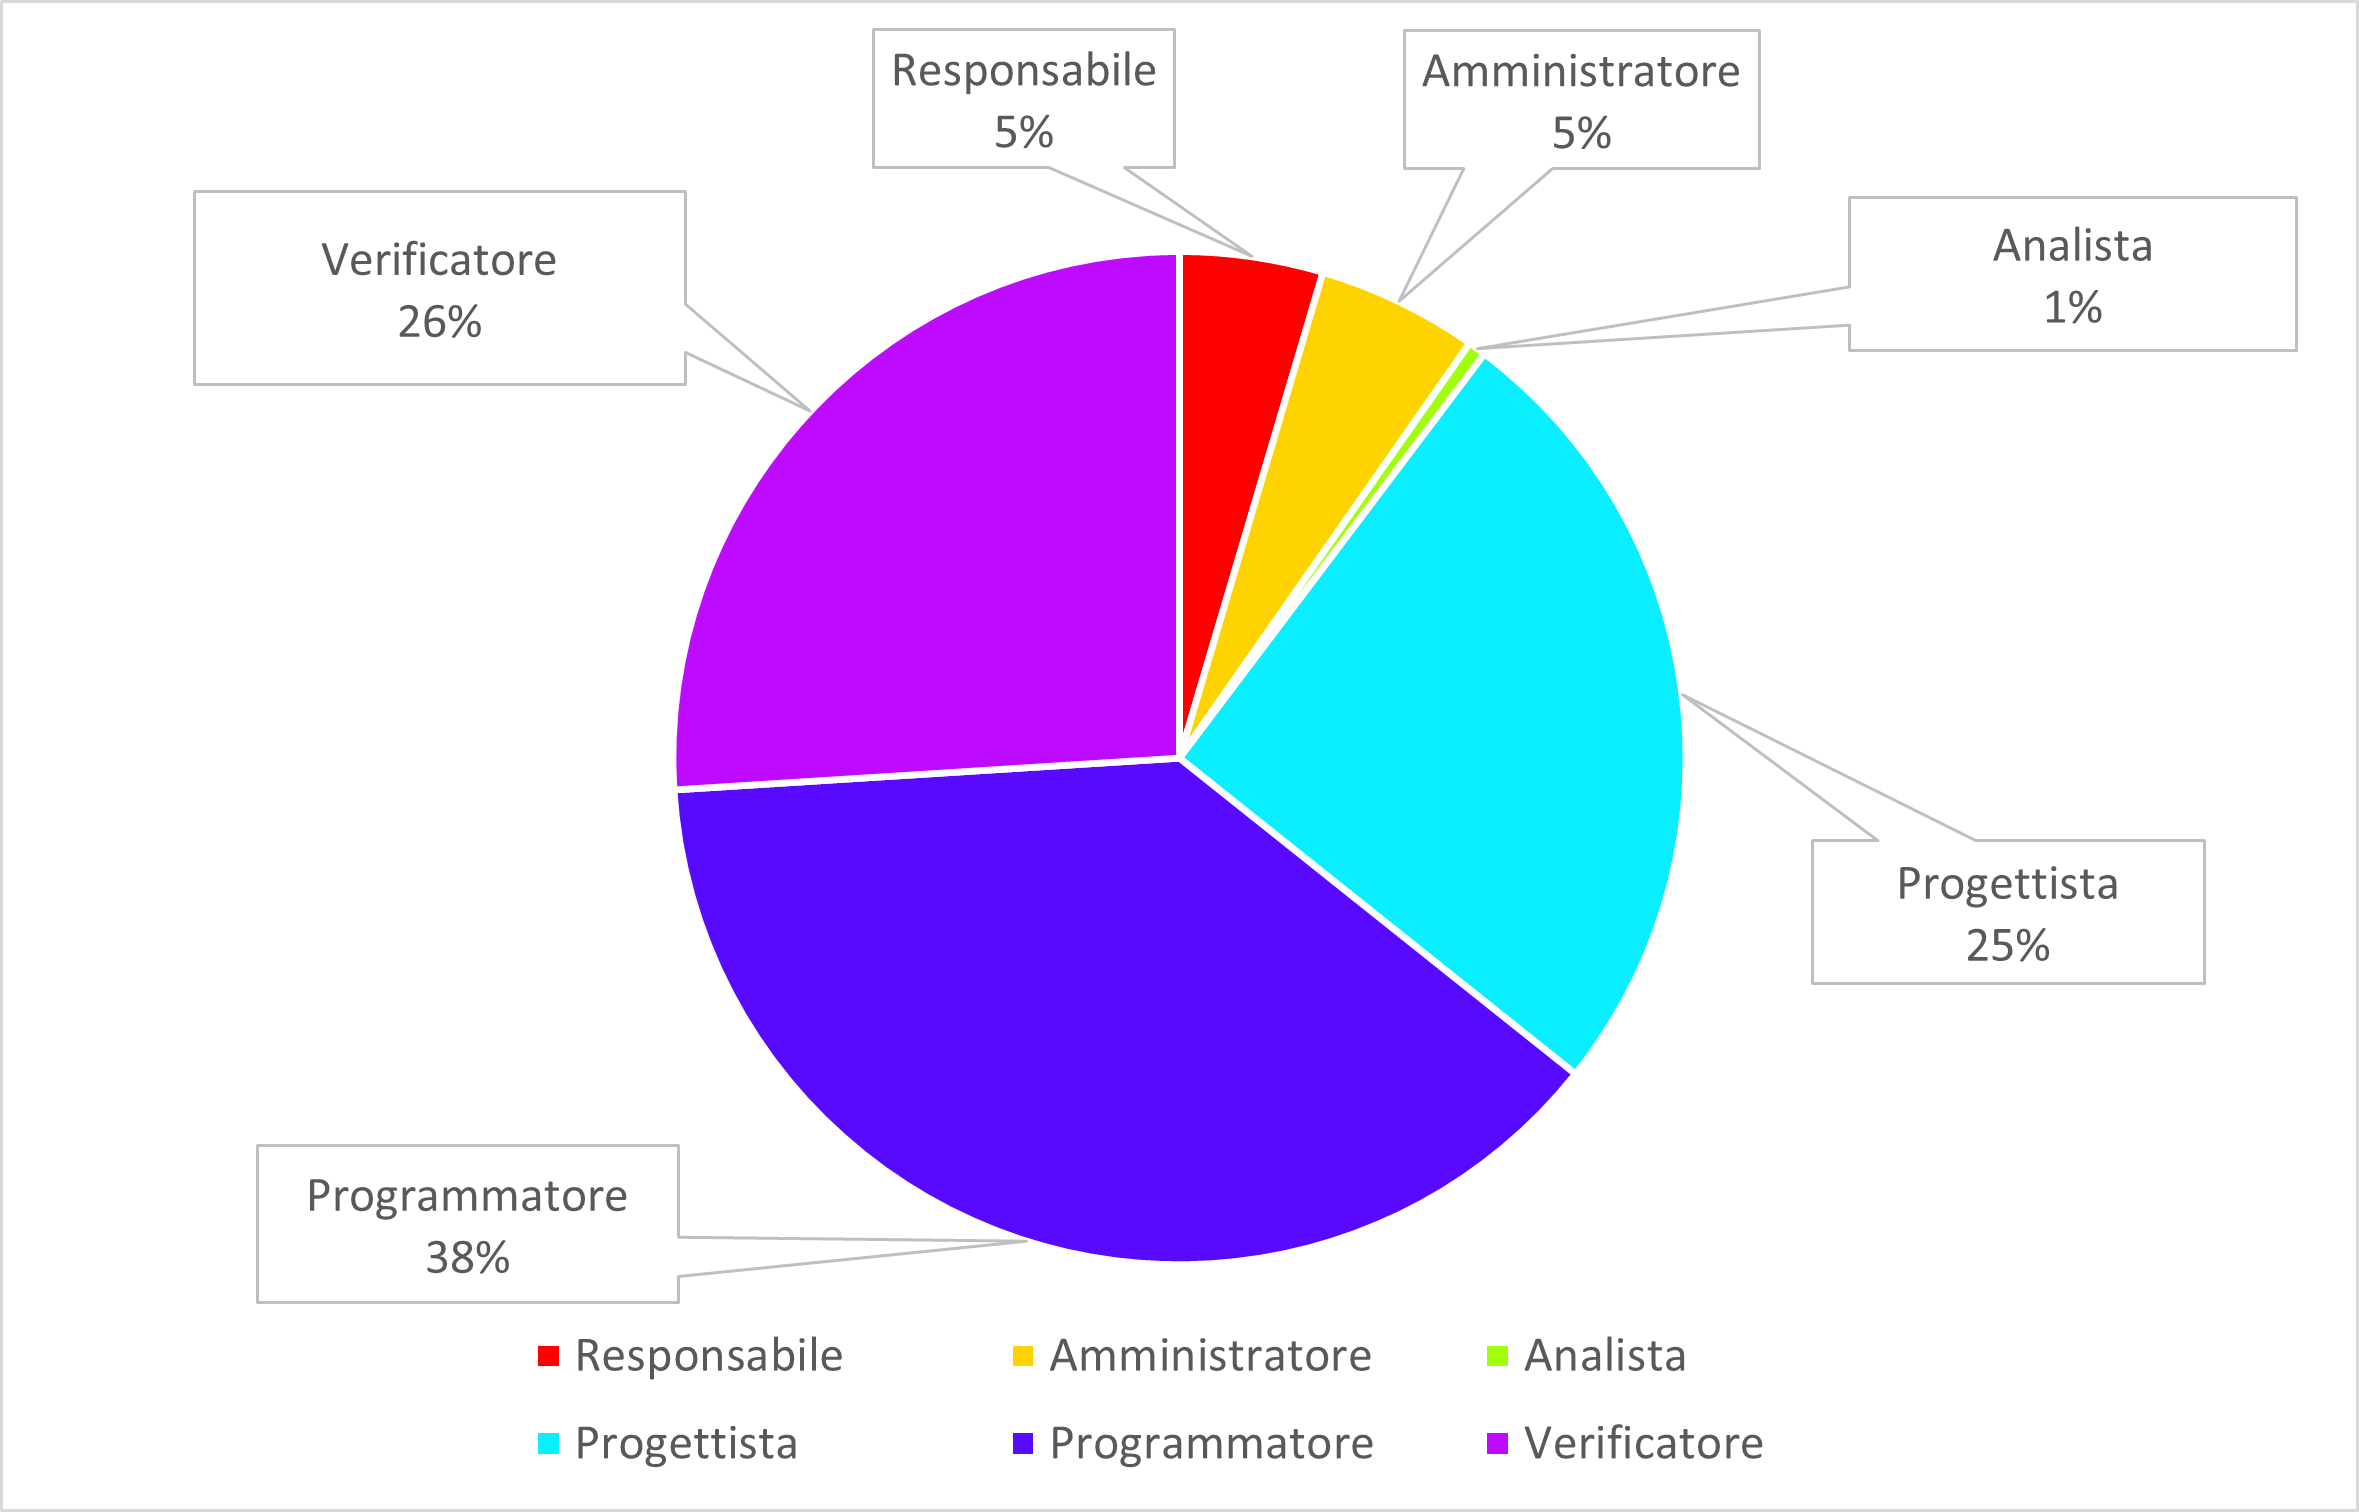
\includegraphics[scale = 0.5]{components/img/Sprint-8-9-torta.png}
    \caption{ Areogramma della ripartizione di ore per ruolo in Progettazione di dettaglio e codifica}
    \label{fig:Areogramma ripartizione ore , fase di Progettazione di dettaglio e codifica}
\end{figure}
\subsection{Fase di Validazione e collaudo}

\subsubsection{Sprint 10}

In questo sprint la distribuzione oraria è la seguente:
\begin{table}[H]
		\begin{center}
			\setlength{\aboverulesep}{0pt}
			\setlength{\belowrulesep}{0pt}
			\setlength{\extrarowheight}{.75ex}
			\rowcolors{2}{AzzurroGruppo!10}{white}
			\begin{tabular}{ c c c c c c c c }
				\rowcolor{AzzurroGruppo!30} 
				\textbf{Nominativo} & \textbf{Re} & \textbf{Am} & \textbf{An} & \textbf{Pt} & \textbf{Pr} & \textbf{Ve} & \textbf{Ore Totali}  \\
				\toprule
				\Davide    & 4 & 5 & - & - & - & 1 & 10 \\
				\Giosue    & - & - & - & 2 & 3 & 5 & 10 \\
				\Francesco & - & 3 & - & - & 4 & 3 & 10\\
				\Daniele   & - & - & - & - & 4 & 6 & 10\\
				\Lucrezia  & - & - & - & - & 7 & 3 & 10\\
				\Matteo    & 4 & - & - & - & - & 6 & 10\\
				\Tommaso   & - & - & - & 5 & - & 5 & 10\\
				 \textbf{Ore totali} & \textbf{8} & \textbf{8} & \textbf{-} & \textbf{7} & \textbf{18} & \textbf{29} & \textbf{70} \\
				\bottomrule
			\end{tabular}
			\caption{Distribuzione delle ore nello sprint 10}
		\end{center}
	\end{table}


\subsubsection{Sprint 11}


In questo sprint la distribuzione oraria è la seguente:
\begin{table}[H]
		\begin{center}
			\setlength{\aboverulesep}{0pt}
			\setlength{\belowrulesep}{0pt}
			\setlength{\extrarowheight}{.75ex}
			\rowcolors{2}{AzzurroGruppo!10}{white}
			\begin{tabular}{ c c c c c c c c }
				\rowcolor{AzzurroGruppo!30} 
				\textbf{Nominativo} & \textbf{Re} & \textbf{Am} & \textbf{An} & \textbf{Pt} & \textbf{Pr} & \textbf{Ve} & \textbf{Ore Totali}  \\
				\toprule
				\Davide    & - & - & - & - & 5 & 5 & 10 \\
				\Giosue    & - & - & - & 2 & 3 & 5 & 10 \\
				\Francesco & - & 3 & - & - & 4 & 3 & 10\\
				\Daniele   & 4 & - & - & - & - & 6 & 10\\
				\Lucrezia  & 5 & - & - & - & - & 5 & 10\\
				\Matteo    & - & - & - & - & 6 & 4 & 10\\
				\Tommaso   & - & 5 & - & - & - & 5 & 10\\
				 \textbf{Ore totali} & \textbf{9} & \textbf{8} & \textbf{-} & \textbf{2} & \textbf{18} & \textbf{33} & \textbf{70} \\
				\bottomrule
			\end{tabular}
			\caption{Distribuzione delle ore nello sprint 11}
		\end{center}
	\end{table}


\subsubsection{Prospetto orario}
In questa fase la distribuzione oraria è la seguente:
\begin{table}[H]
		\begin{center}
			\setlength{\aboverulesep}{0pt}
			\setlength{\belowrulesep}{0pt}
			\setlength{\extrarowheight}{.75ex}
			\rowcolors{2}{AzzurroGruppo!10}{white}
			\begin{tabular}{ c c c c c c c c }
				\rowcolor{AzzurroGruppo!30} 
				\textbf{Nominativo} & \textbf{Re} & \textbf{Am} & \textbf{An} & \textbf{Pt} & \textbf{Pr} & \textbf{Ve} & \textbf{Ore Totali}  \\
				\toprule
				\Davide    & 4 & 5 & - & - & 5 & 6 & 20 \\
				\Giosue    & - & - & - & 4 & 6 & 10 & 20 \\
				\Francesco & - & 6 & - & - & 8 & 6 & 20\\
				\Daniele   & 4 & - & - & - & 4 & 12 & 20\\
				\Lucrezia  & 5 & - & - & - & 7 & 8 & 20\\
				\Matteo    & 4 & - & - & - & 6 & 10 & 20\\
				\Tommaso   & - & 5 & - & 5 & - & 10 & 20\\
				 \textbf{Ore totali} & \textbf{17} & \textbf{16} & \textbf{-} & \textbf{9} & \textbf{36} & \textbf{62} & \textbf{140} \\
				\bottomrule
			\end{tabular}
			\caption{Distribuzione delle ore nel periodo di Validazione e collaudo}
		\end{center}
	\end{table}
	I dati ottenuti vengono riassunti nel seguente istogramma:
	\begin{figure}[H]
    \centering
    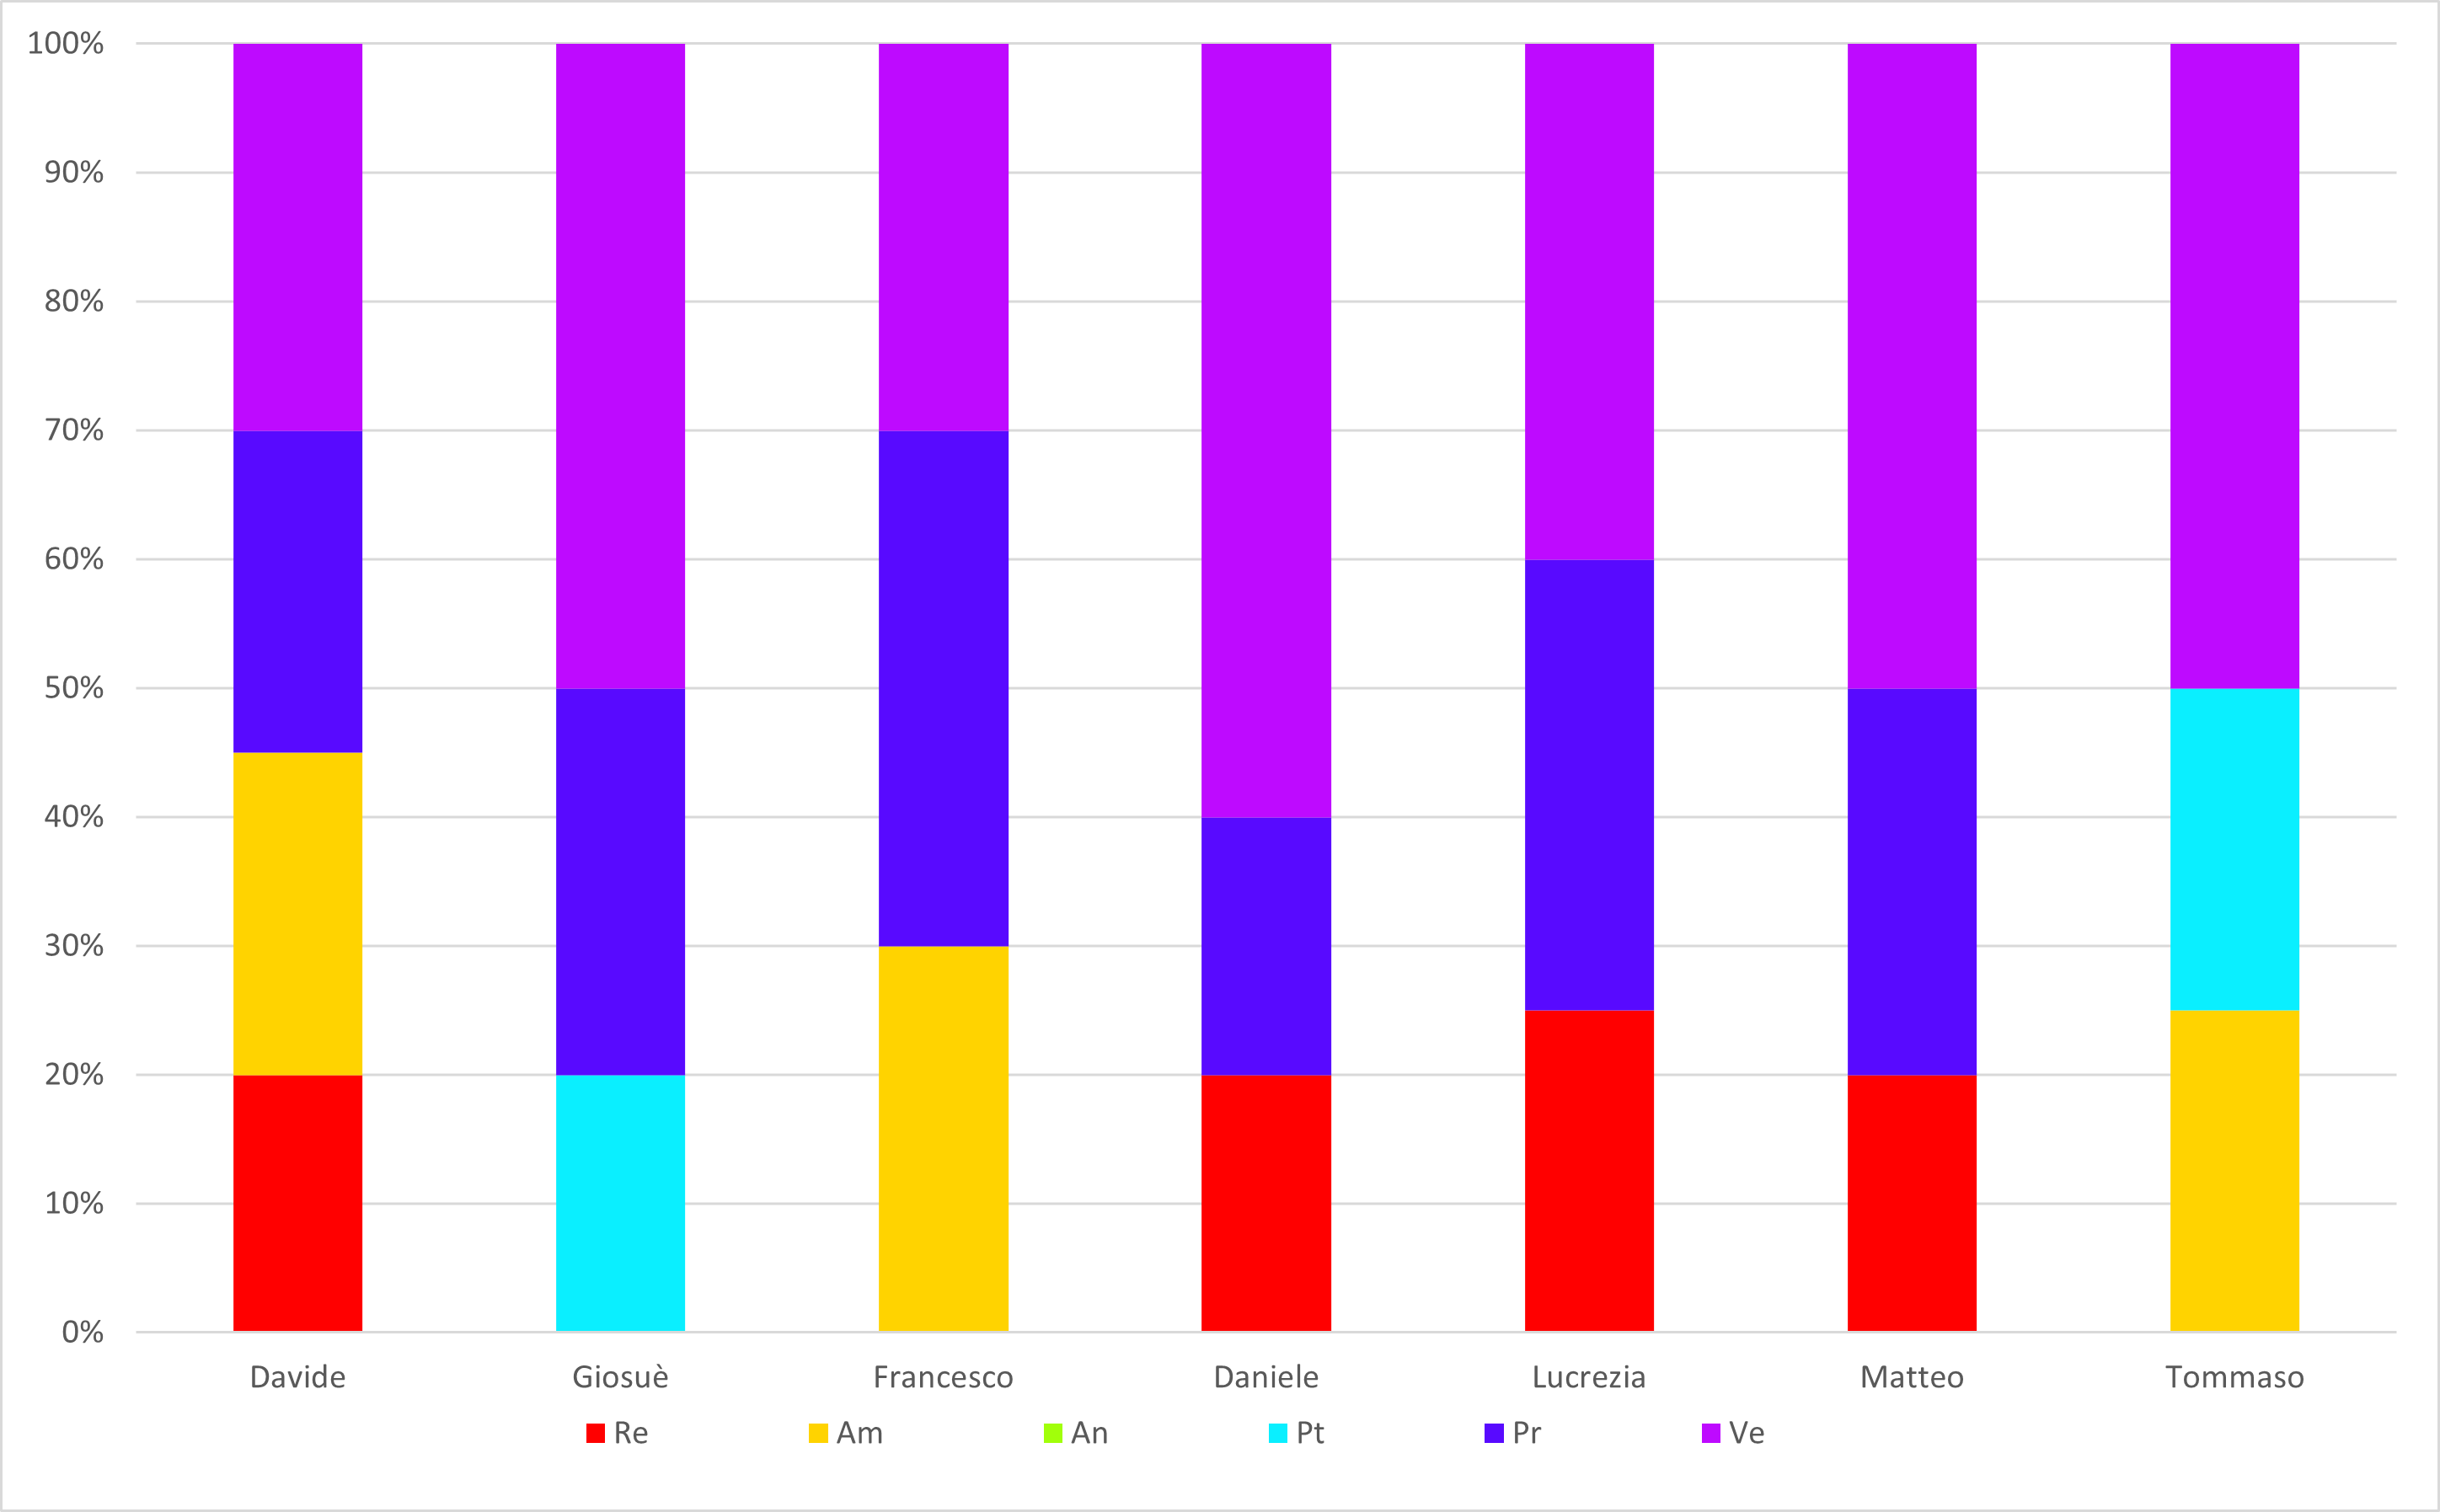
\includegraphics[scale = 0.5]{components/img/Sprint-10-11-isto.png}
    \caption{Istogramma della ripartizione di ore per ruolo in Validazione e collaudo}
    \label{fig:istogramma ripartizione ore , fase di Validazione e Collaudo}
\end{figure}
\subsubsection{Prospetto economico}
Il costo per ogni ruolo è il seguente:
\begin{table}[H]
		\begin{center}
			\setlength{\aboverulesep}{0pt}
			\setlength{\belowrulesep}{0pt}
			\setlength{\extrarowheight}{.75ex}
			\rowcolors{2}{AzzurroGruppo!10}{white}
			\begin{tabular}{ c c c }
				\rowcolor{AzzurroGruppo!30} 
				\textbf{Ruolo} & \textbf{Ore} & \textbf{Costo}  \\
				\toprule
				Responsabile   & 17 & 510 \euro \\
				Amministratore & 16 & 320 \euro \\
				Analista       & -  & - \\
				Progettista    & 9  & 198 \euro \\
				Programmatore  & 36 & 540 \euro \\
				Verificatore   & 62 & 930 \euro \\
				\textbf{Totale} & \textbf{140} & \textbf{2498 \euro} \\
				\bottomrule
			\end{tabular}
			\caption{ Prospetto dei costi per ruoli nel periodo di Validazione e collaudo}
		\end{center}
	\end{table}
I dati ottenuti si possono riassumere nel seguente areogramma:
\begin{figure}[H]
    \centering
    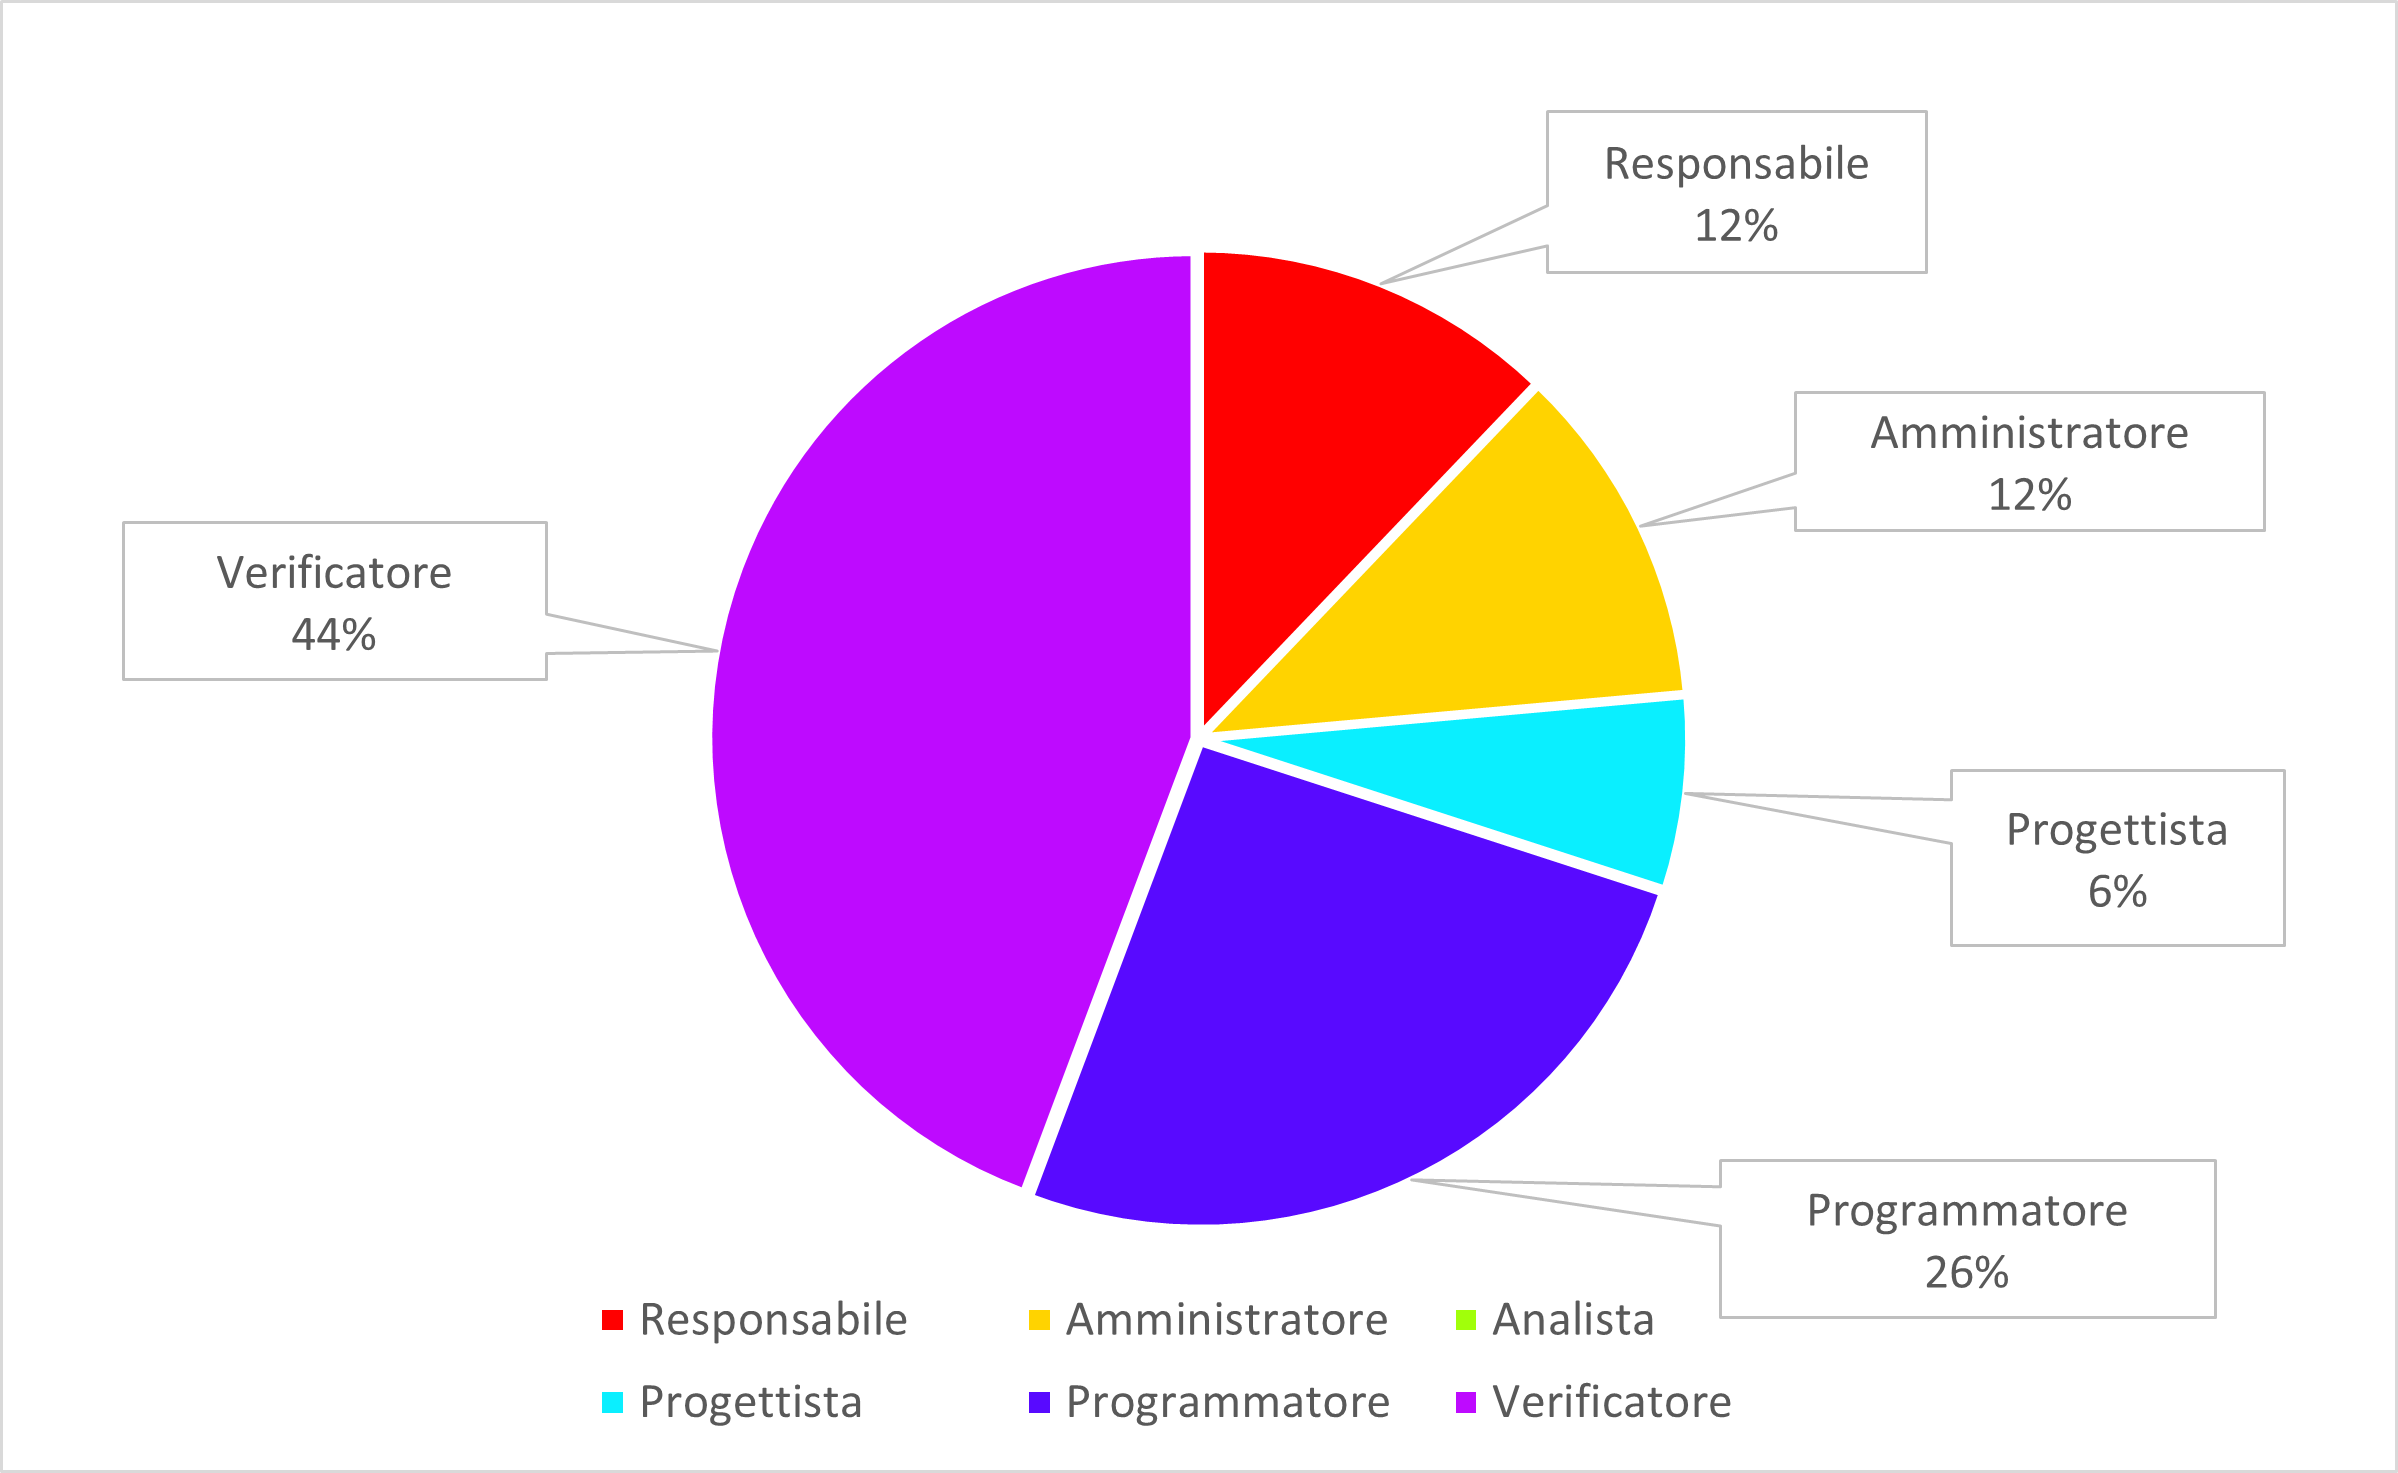
\includegraphics[scale = 0.5]{components/img/Sprint-10-11-torta.png}
    \caption{ Areogramma della ripartizione di ore per ruolo in Validazione e collaudo}
    \label{fig:Areogramma ripartizione ore , fase di Validazione e collaudo}
\end{figure}
\subsection{Riepilogo}
\subsubsection{Ore totali}
\paragraph{Suddivisione del lavoro}
Nella seguente tabella vengono riportate il totale delle ore del progetto, sono presenti sia le ore di investimento, sia le ore rendicontate a carico del committente.
\begin{table}[H]
		\begin{center}
			\setlength{\aboverulesep}{0pt}
			\setlength{\belowrulesep}{0pt}
			\setlength{\extrarowheight}{.75ex}
			\rowcolors{2}{AzzurroGruppo!10}{white}
			\begin{tabular}{ c c c c c c c c }
				\rowcolor{AzzurroGruppo!30} 
				\textbf{Nominativo} & \textbf{Re} & \textbf{Am} & \textbf{An} & \textbf{Pt} & \textbf{Pr} & \textbf{Ve} & \textbf{Ore Totali}  \\
				\toprule
				\Davide    & 9 & 16 & 18 & 15 & 29 & 48 & 135 \\
				\Giosue    & 7 & 10 & 17 & 26 & 32 & 43 & 135 \\
				\Francesco & 13 & 14 & 23 & 24 & 31 & 30 & 135\\
				\Daniele   & 14 & 6 & 22 & 28 & 22 & 43 & 135\\
				\Lucrezia  & 18 & 11 & 17 & 15 & 26 & 48 & 135\\
				\Matteo    & 18 & 13 & 17 & 27 & 27 & 33 & 135\\
				\Tommaso   & 4 & 19 & 26 & 24 & 24 & 38 & 135\\
				 \textbf{Ore totali} & \textbf{83} & \textbf{89} & \textbf{140} & \textbf{159} & \textbf{191} & \textbf{283} & \textbf{945} \\
				\bottomrule
			\end{tabular}
			\caption{ Distribuzione delle ore totali di investimento e rendicontate}
		\end{center}
	\end{table}
	I dati ottenuti vengono riassunti nel seguente istogramma:
\begin{figure}[H]
    \centering
    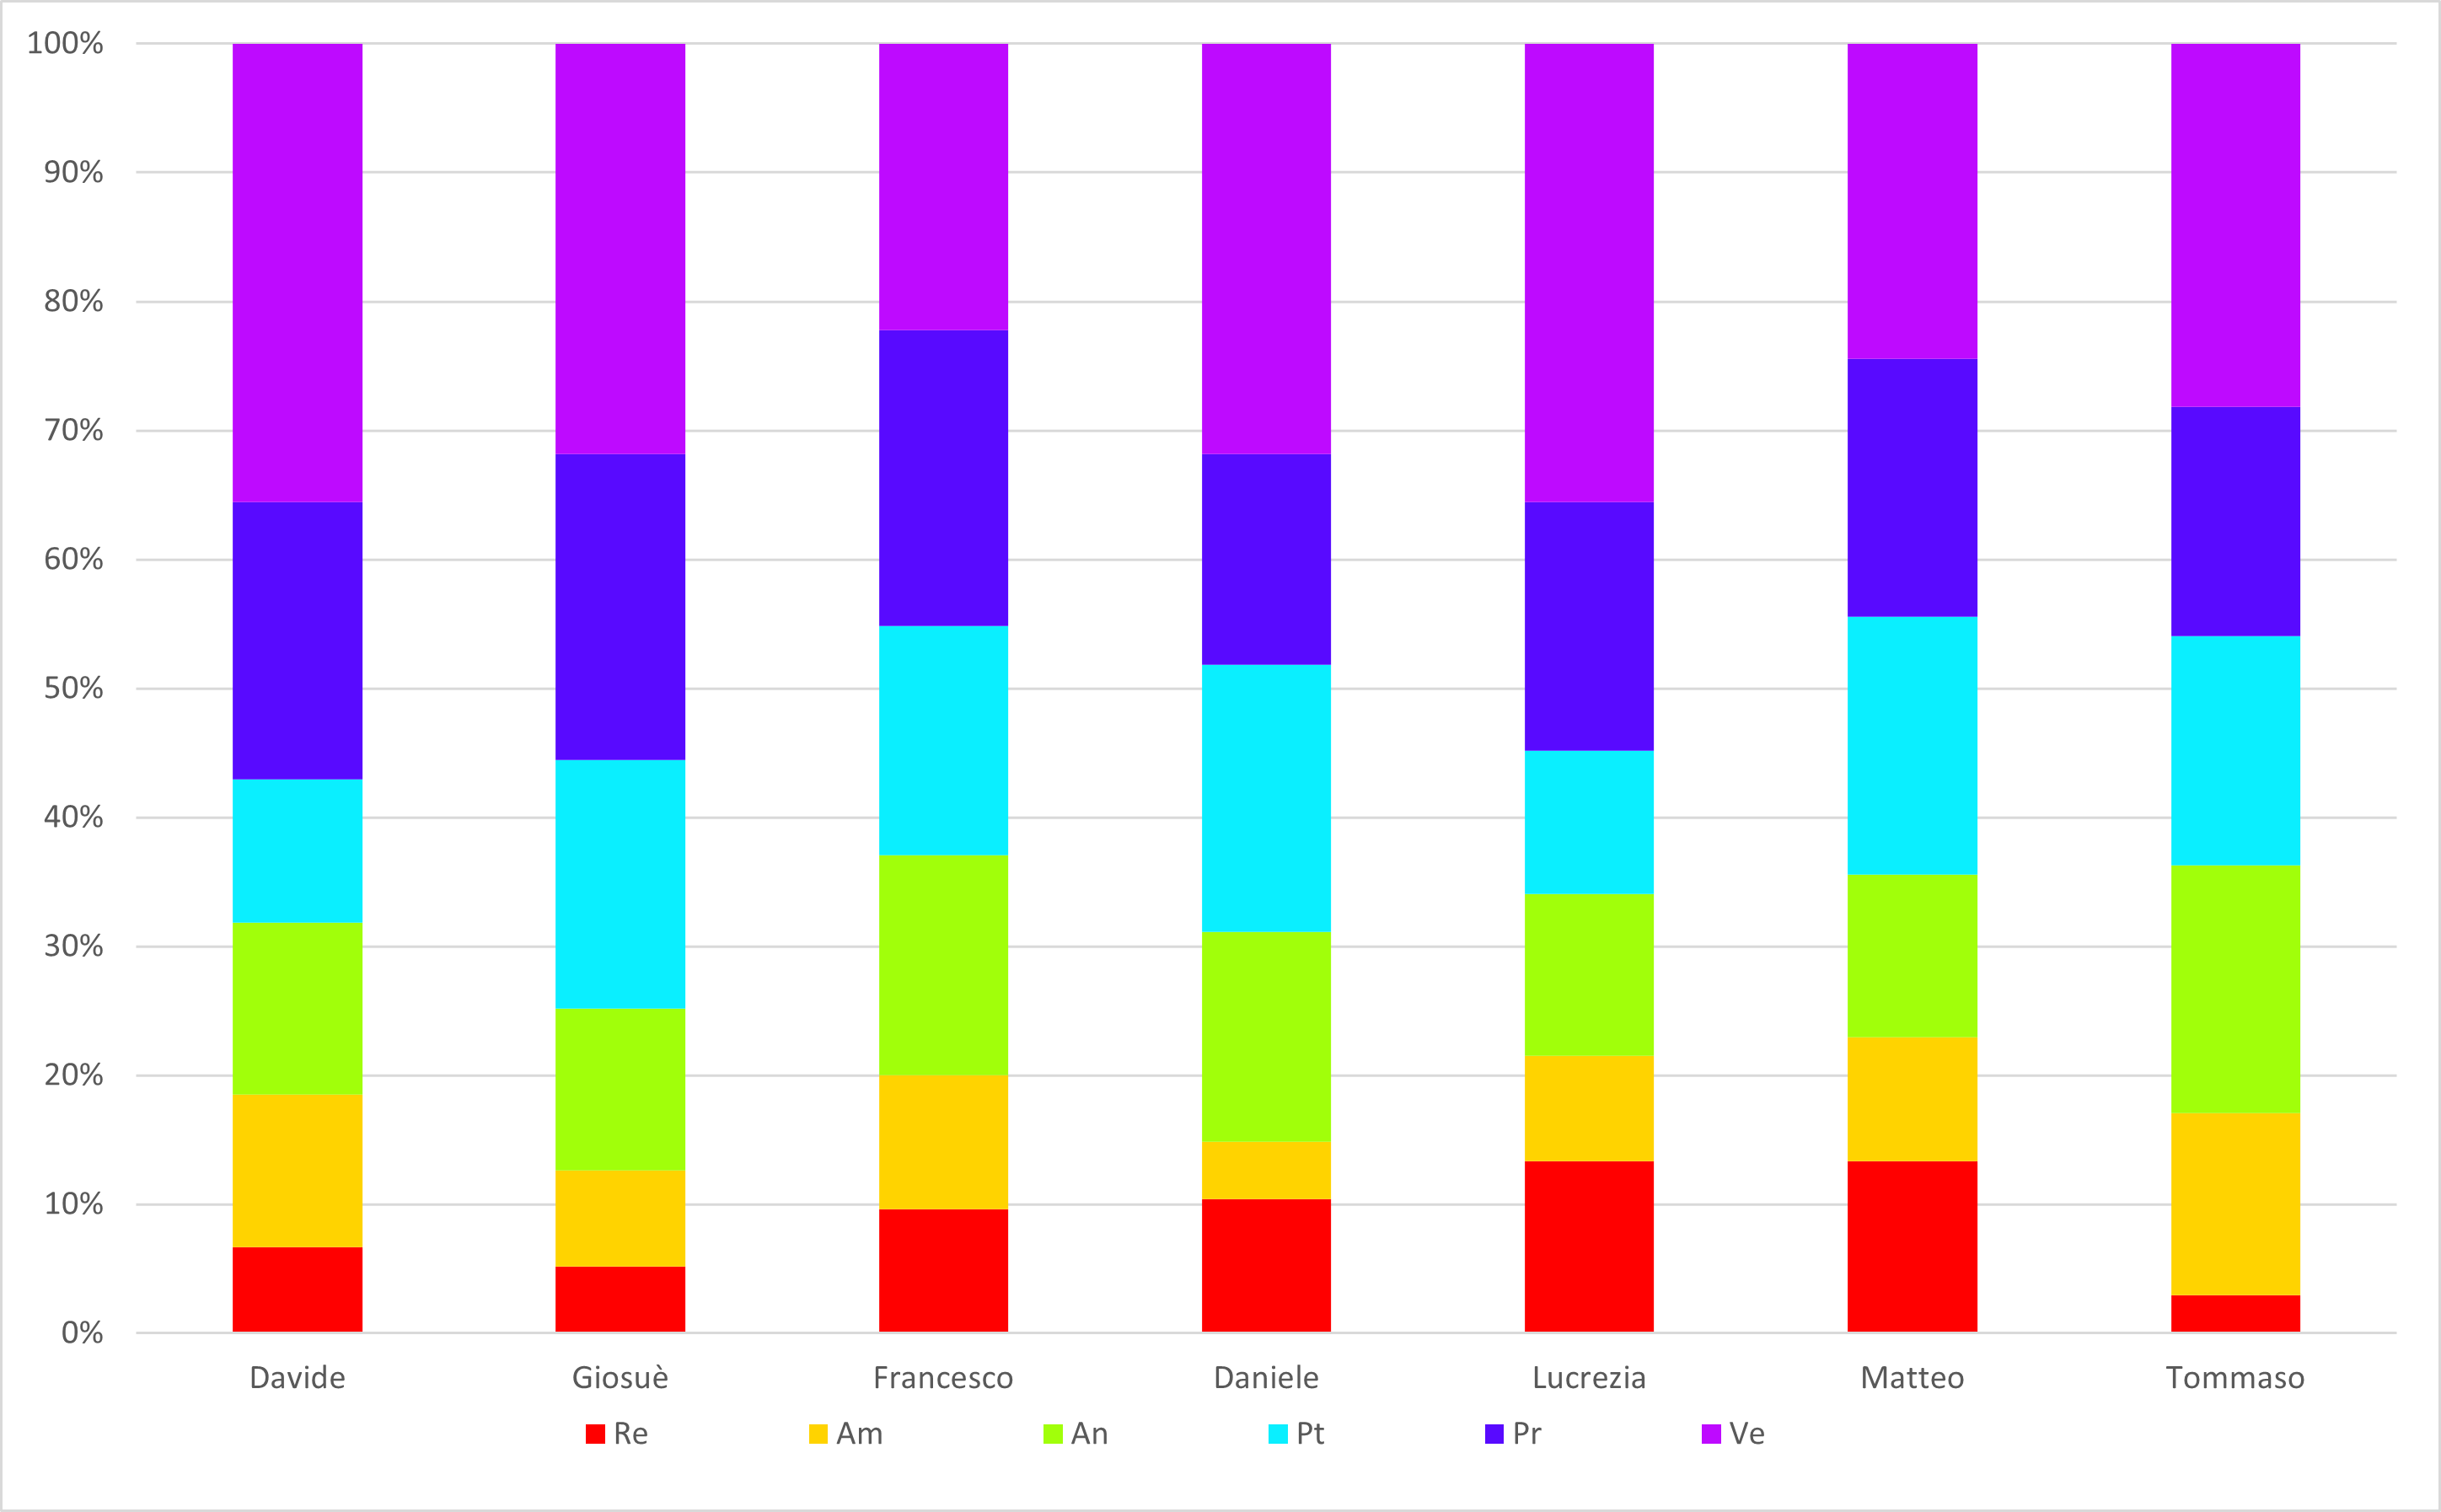
\includegraphics[scale = 0.5]{components/img/Totale-non-rendicontate-isto.png}
    \caption{ Istogramma della ripartizione di ore totali di investimento e rendicontate}
    \label{fig:Istogramma ripartizione ore totali di investimento e rendicontate }
\end{figure}
\paragraph{Prospetto economico}
Il costo per ogni ruolo è il seguente:
\begin{table}[H]
		\begin{center}
			\setlength{\aboverulesep}{0pt}
			\setlength{\belowrulesep}{0pt}
			\setlength{\extrarowheight}{.75ex}
			\rowcolors{2}{AzzurroGruppo!10}{white}
			\begin{tabular}{ c c c }
				\rowcolor{AzzurroGruppo!30} 
				\textbf{Ruolo} & \textbf{Ore} & \textbf{Costo}  \\
				\toprule
				Responsabile   & 85 & 2550 \euro \\
				Amministratore & 89 & 1780 \euro \\
				Analista       & 138 & 3450 \euro \\
				Progettista    & 159 & 3498 \euro \\
				Programmatore  & 191 & 2865 \euro \\
				Verificatore   & 283 & 4245 \euro \\
				\textbf{Totale} & \textbf{945} & \textbf{18388 \euro} \\
				\bottomrule
			\end{tabular}
			\caption{ Prospetto dei costi totale delle ore di investimento e rendicontate}
		\end{center}
	\end{table}
I dati ottenuti si possono riassumere nel seguente areogramma:
\begin{figure}[H]
    \centering
    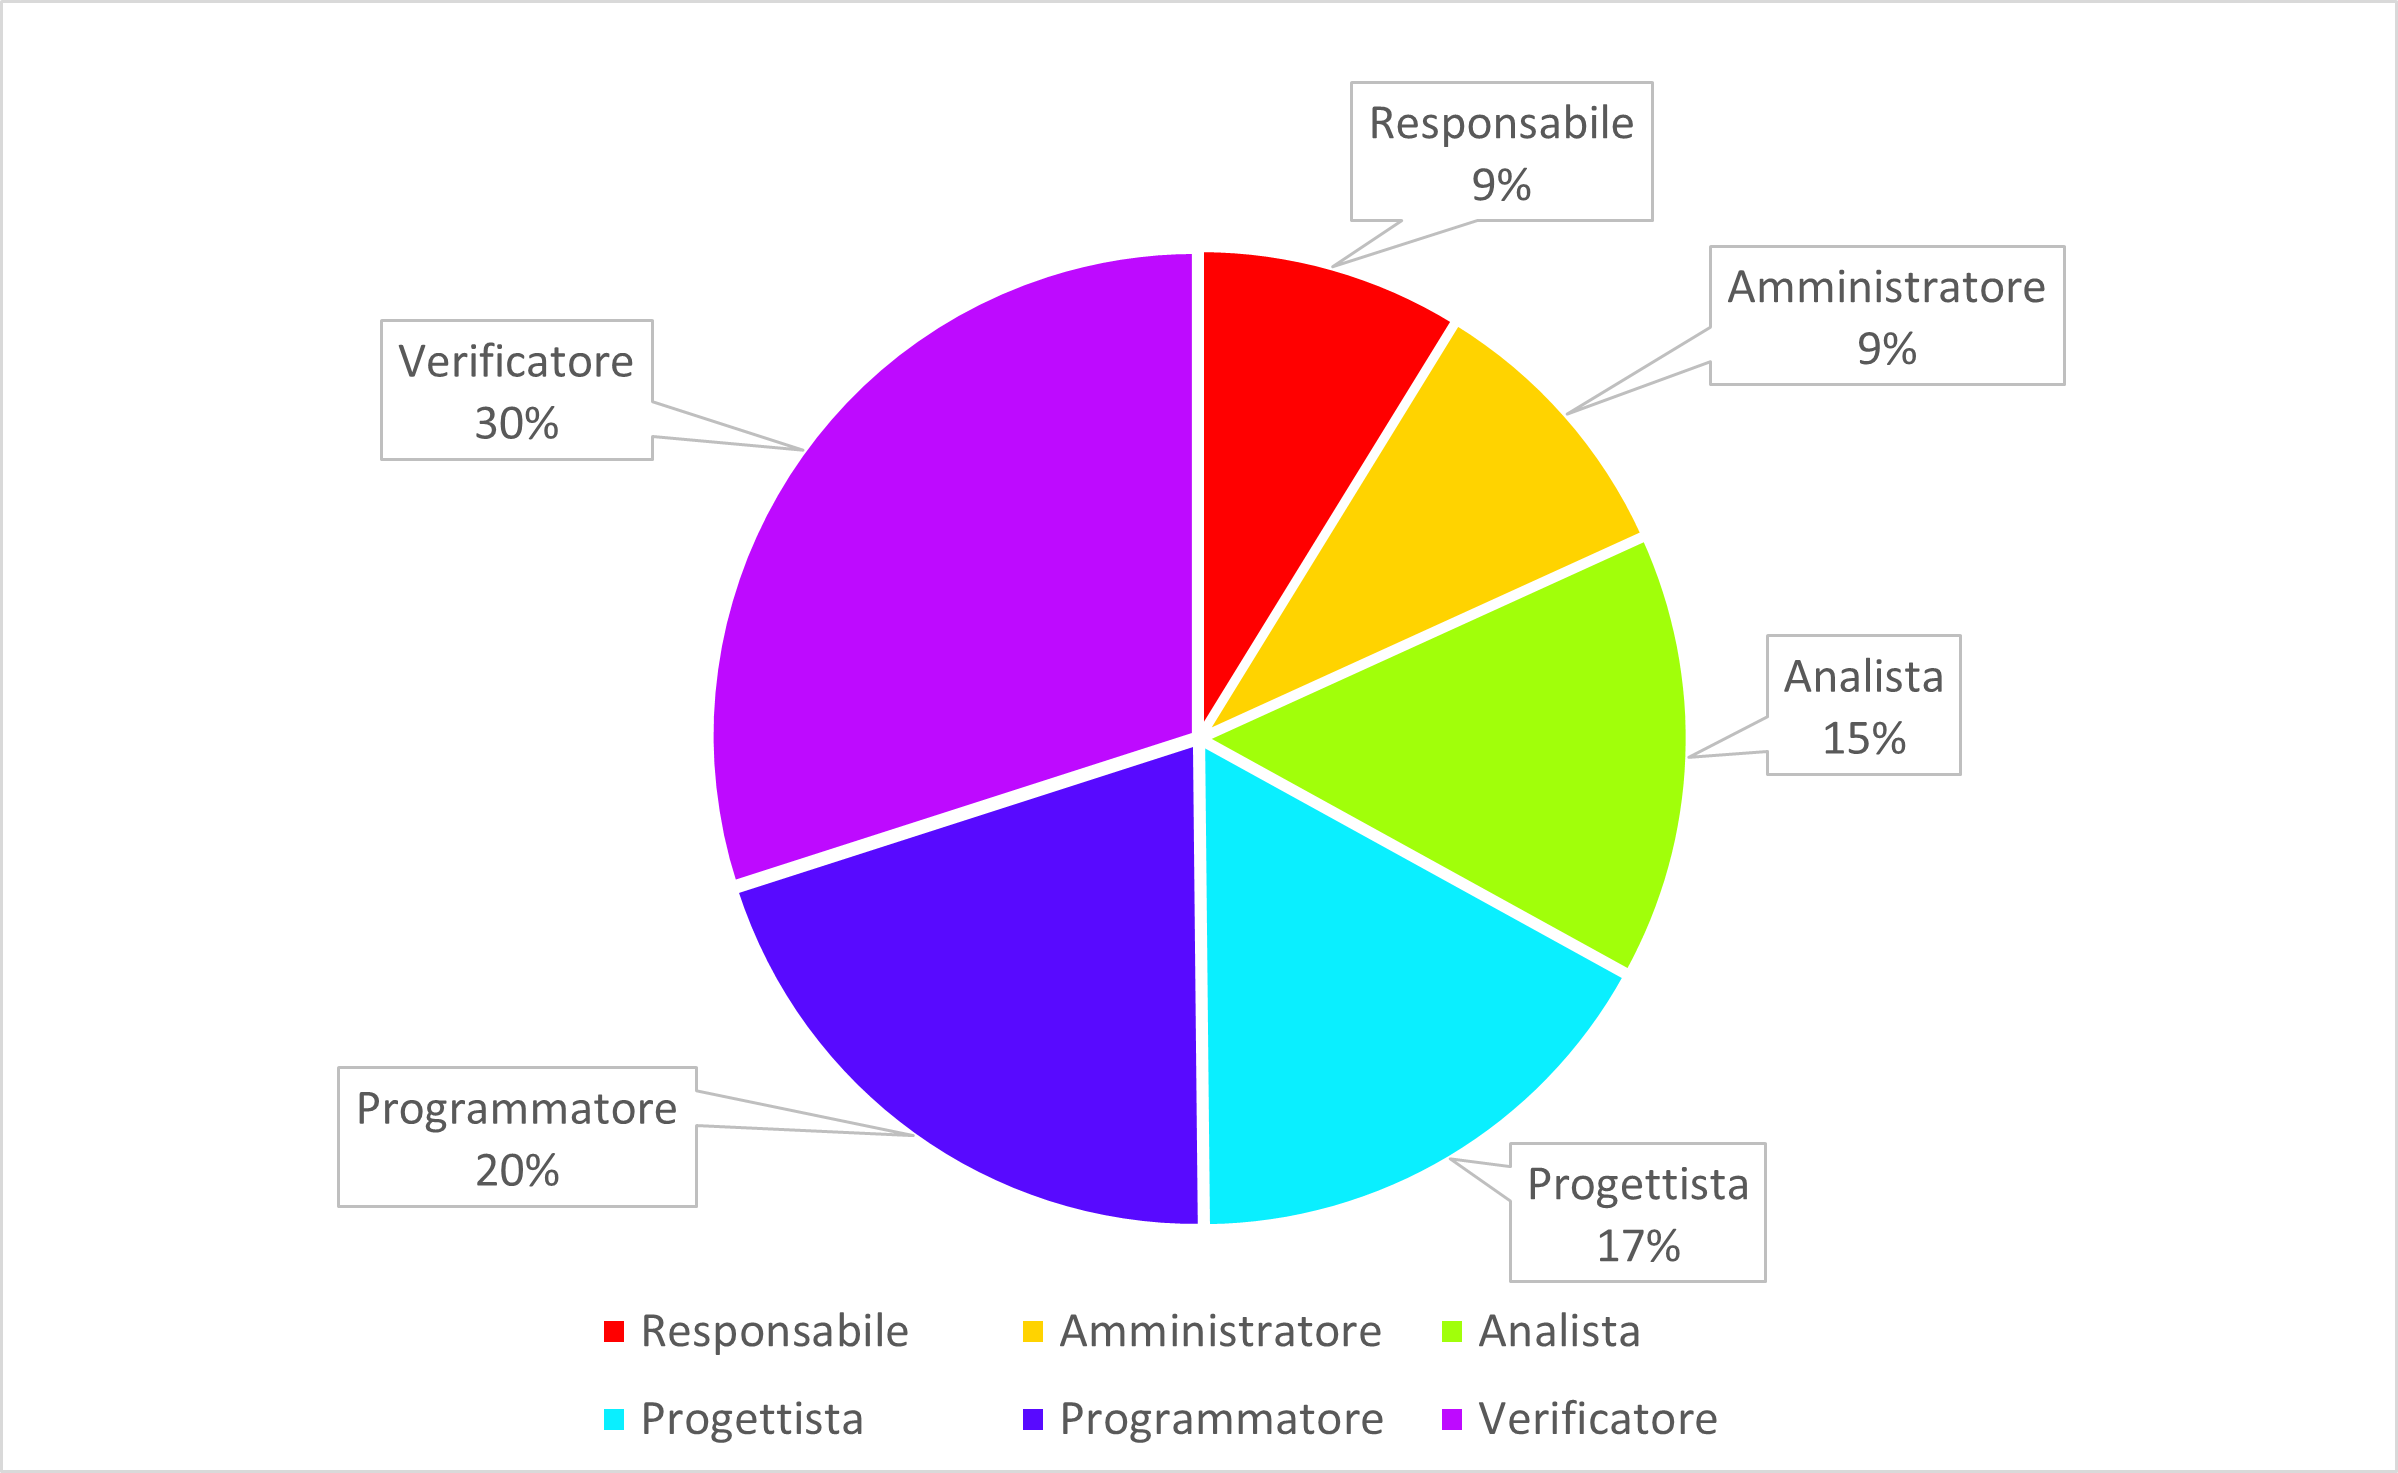
\includegraphics[scale = 0.5]{components/img/Totale-non-rendicontate-torta.png}
    \caption{ Areogramma dei costi totale delle ore di investimento e rendicontate}
    \label{fig:areogramma ripartizione ore totali di investimento e rendicontate}
\end{figure}
\subsubsection{Ore rendicontate}
\paragraph{Suddivisione del lavoro}
Nella seguente tabella sono riassunte le ore rendicontate:
\begin{table}[H]
		\begin{center}
			\setlength{\aboverulesep}{0pt}
			\setlength{\belowrulesep}{0pt}
			\setlength{\extrarowheight}{.75ex}
			\rowcolors{2}{AzzurroGruppo!10}{white}
			\begin{tabular}{ c c c c c c c c }
				\rowcolor{AzzurroGruppo!30} 
				\textbf{Nominativo} & \textbf{Re} & \textbf{Am} & \textbf{An} & \textbf{Pt} & \textbf{Pr} & \textbf{Ve} & \textbf{Ore Totali}  \\
				\toprule
				\Davide    & 9  & 11 & -  & 15  & 29 & 36 & 100 \\
				\Giosue    & 7  & 2 & -  & 26 & 32 & 33  & 100 \\
				\Francesco & 4  & 10 & 8  & 24 & 31 & 23  & 100\\
				\Daniele   & 4  & 3 & 11 & 28 & 22 & 31  & 100\\
				\Lucrezia  & 5  & 8 & 10 & 15  & 26 & 36 & 100\\
				\Matteo    & 18 & 8 & -  & 27 & 27 & 20  & 100\\
				\Tommaso   & 4  & 12 & 10 & 24  & 24 & 26  & 100\\
				 \textbf{Ore totali} & \textbf{51} & \textbf{54} & \textbf{40} & \textbf{159} & \textbf{191} & \textbf{205} & \textbf{700} \\
				\bottomrule
			\end{tabular}
			\caption{Distribuzione delle ore rendicontate}
		\end{center}
	\end{table}
	I dati ottenuti vengono riassunti nel seguente istogramma:
\begin{figure}[H]
    \centering
    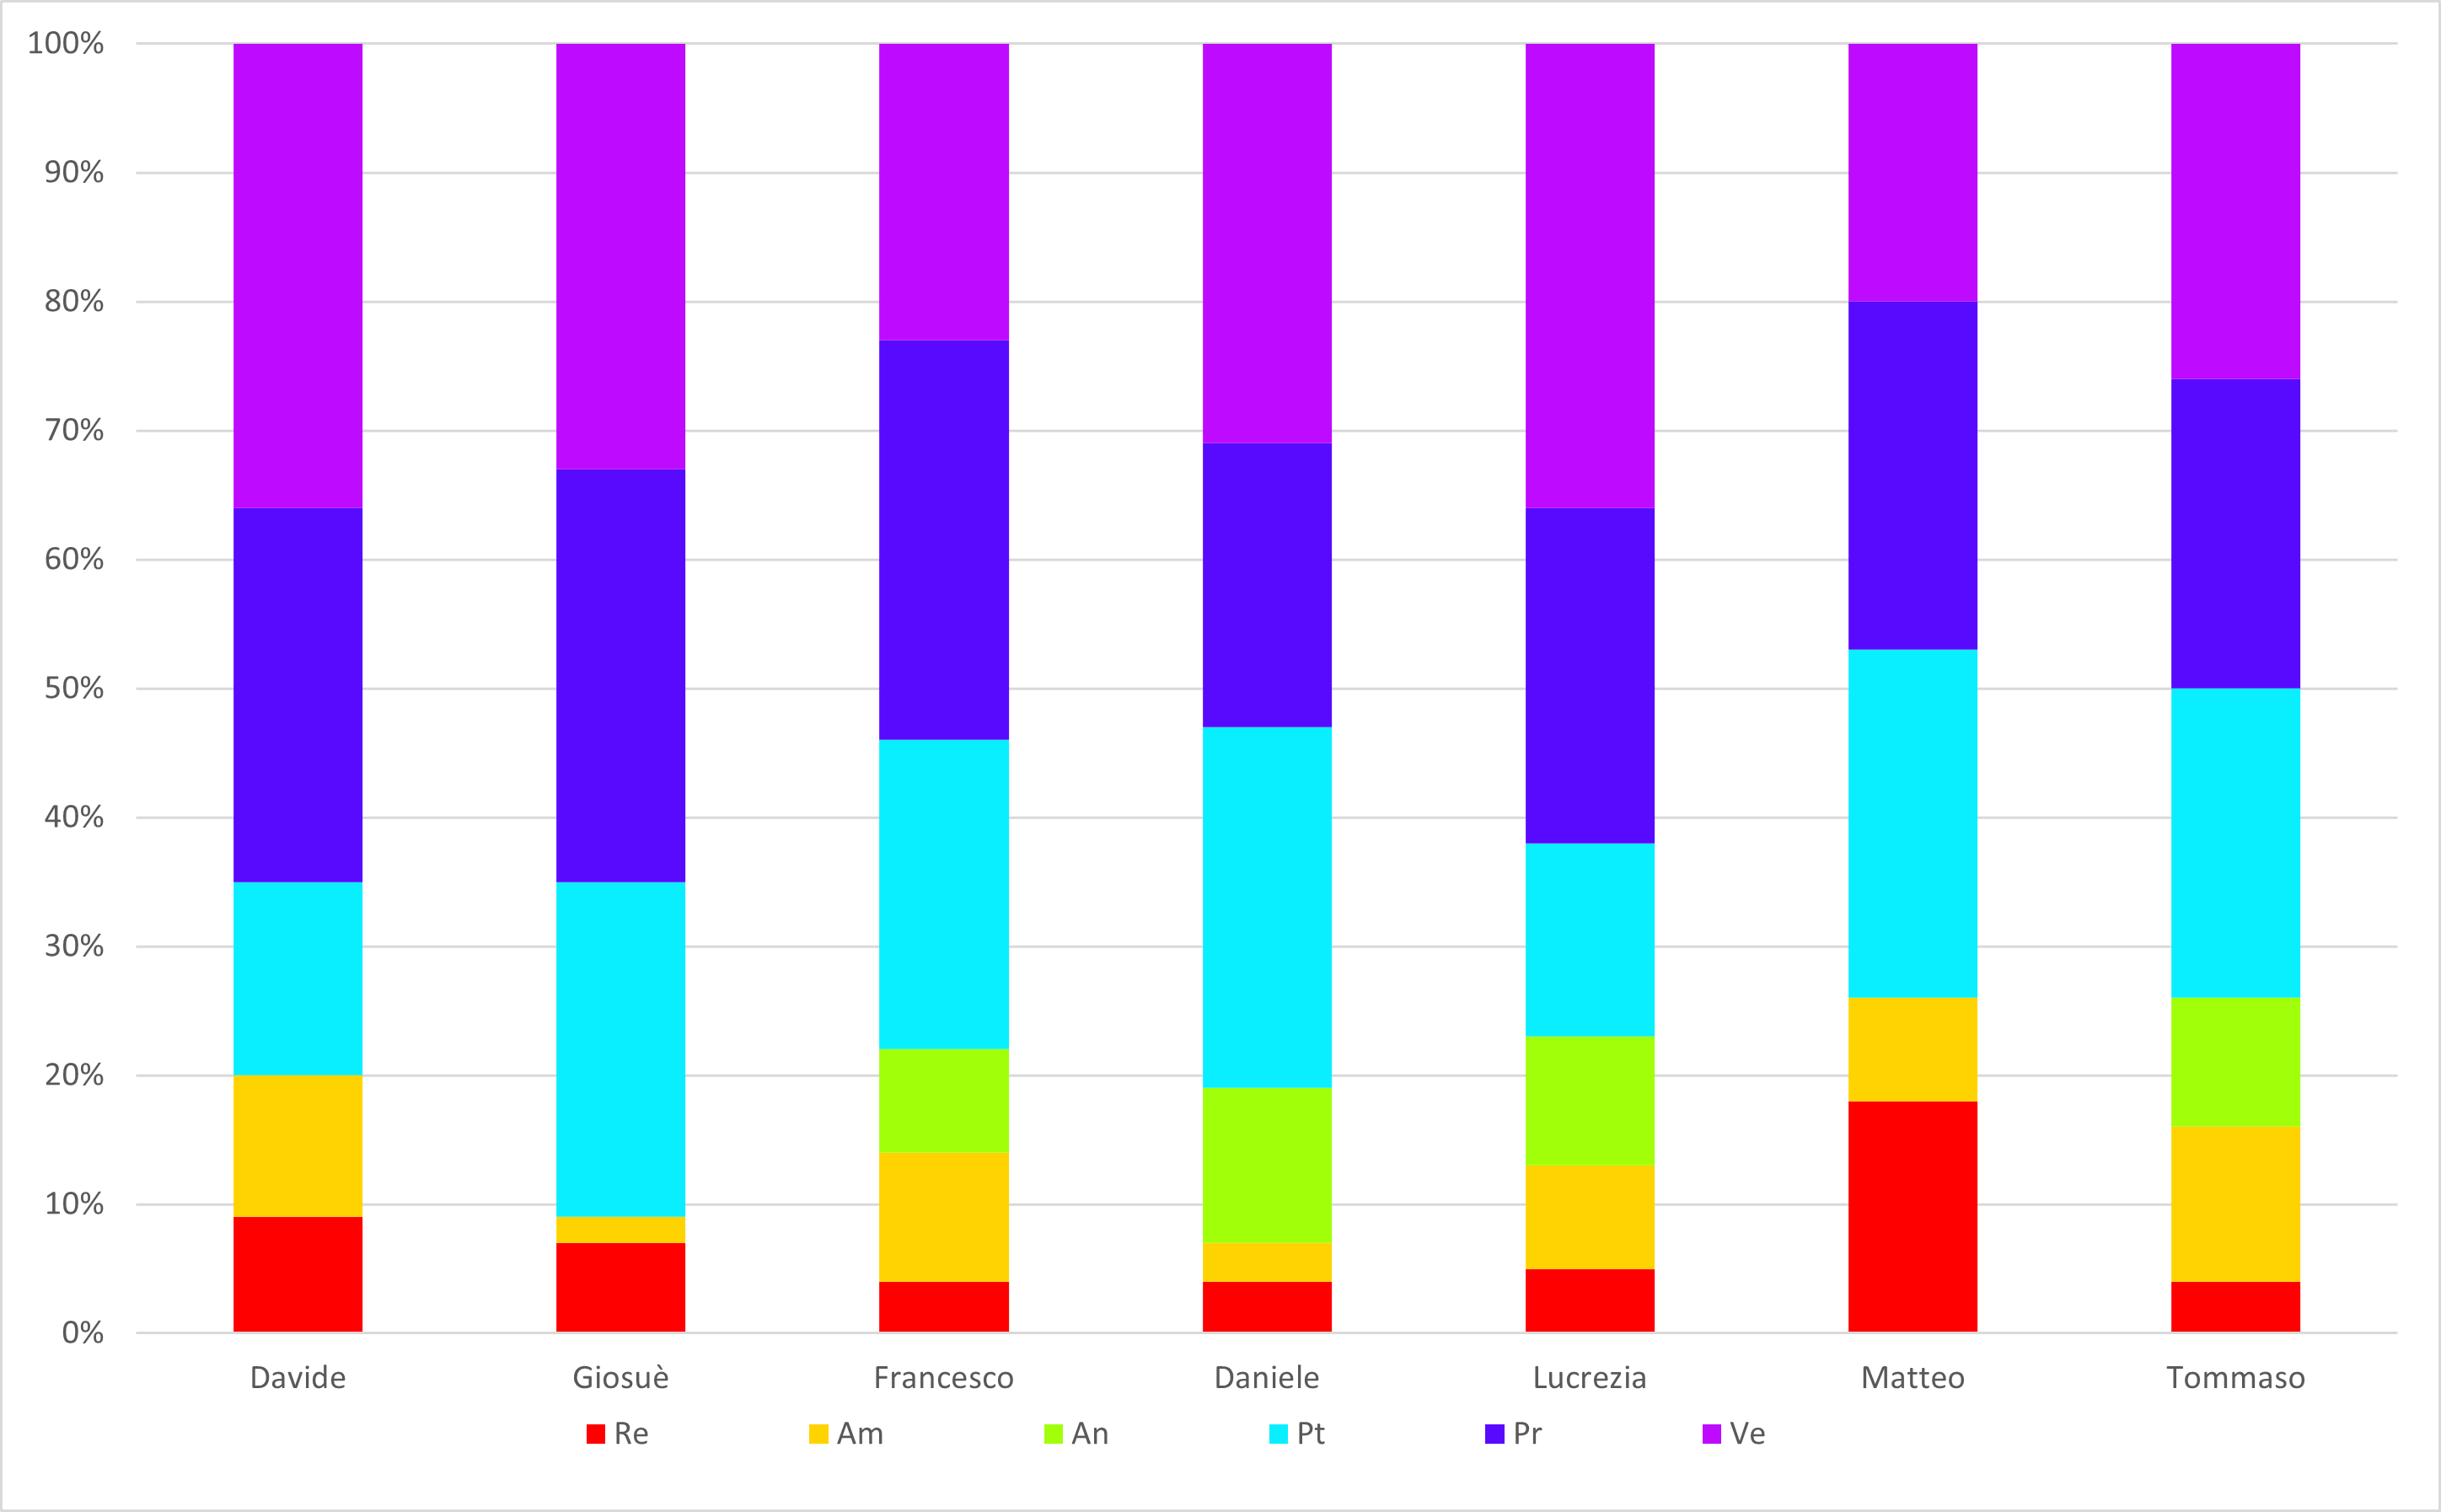
\includegraphics[scale = 0.5]{components/img/Totale-rendicontate-isto.png}
    \caption{ Istogramma della ripartizione delle ore rendicontate}
    \label{fig:Istogramma ripartizione ore totali rendicontate}
\end{figure}
\paragraph{Prospetto economico}
Il costo totale rendicontato per ogni ruolo è il seguente:
\begin{table}[H]
		\begin{center}
			\setlength{\aboverulesep}{0pt}
			\setlength{\belowrulesep}{0pt}
			\setlength{\extrarowheight}{.75ex}
			\rowcolors{2}{AzzurroGruppo!10}{white}
			\begin{tabular}{ c c c }
				\rowcolor{AzzurroGruppo!30} 
				\textbf{Ruolo} & \textbf{Ore} & \textbf{Costo} \\
				\toprule
				Responsabile   & 51 & 1530 \euro \\
				Amministratore & 54 & 1080 \euro \\
				Analista       & 40 & 1000 \euro \\
				Progettista    & 159 & 3498 \euro \\
				Programmatore  & 191 & 2865 \euro \\
				Verificatore   & 205 & 3075 \euro \\
				\textbf{Totale} & \textbf{700} & \textbf{13048 \euro} \\
				\bottomrule
			\end{tabular}
			\caption{Prospetto dei costi delle ore rendicontate}
		\end{center}
	\end{table}
I dati ottenuti si possono riassumere nel seguente areogramma:
\begin{figure}[H]
    \centering
    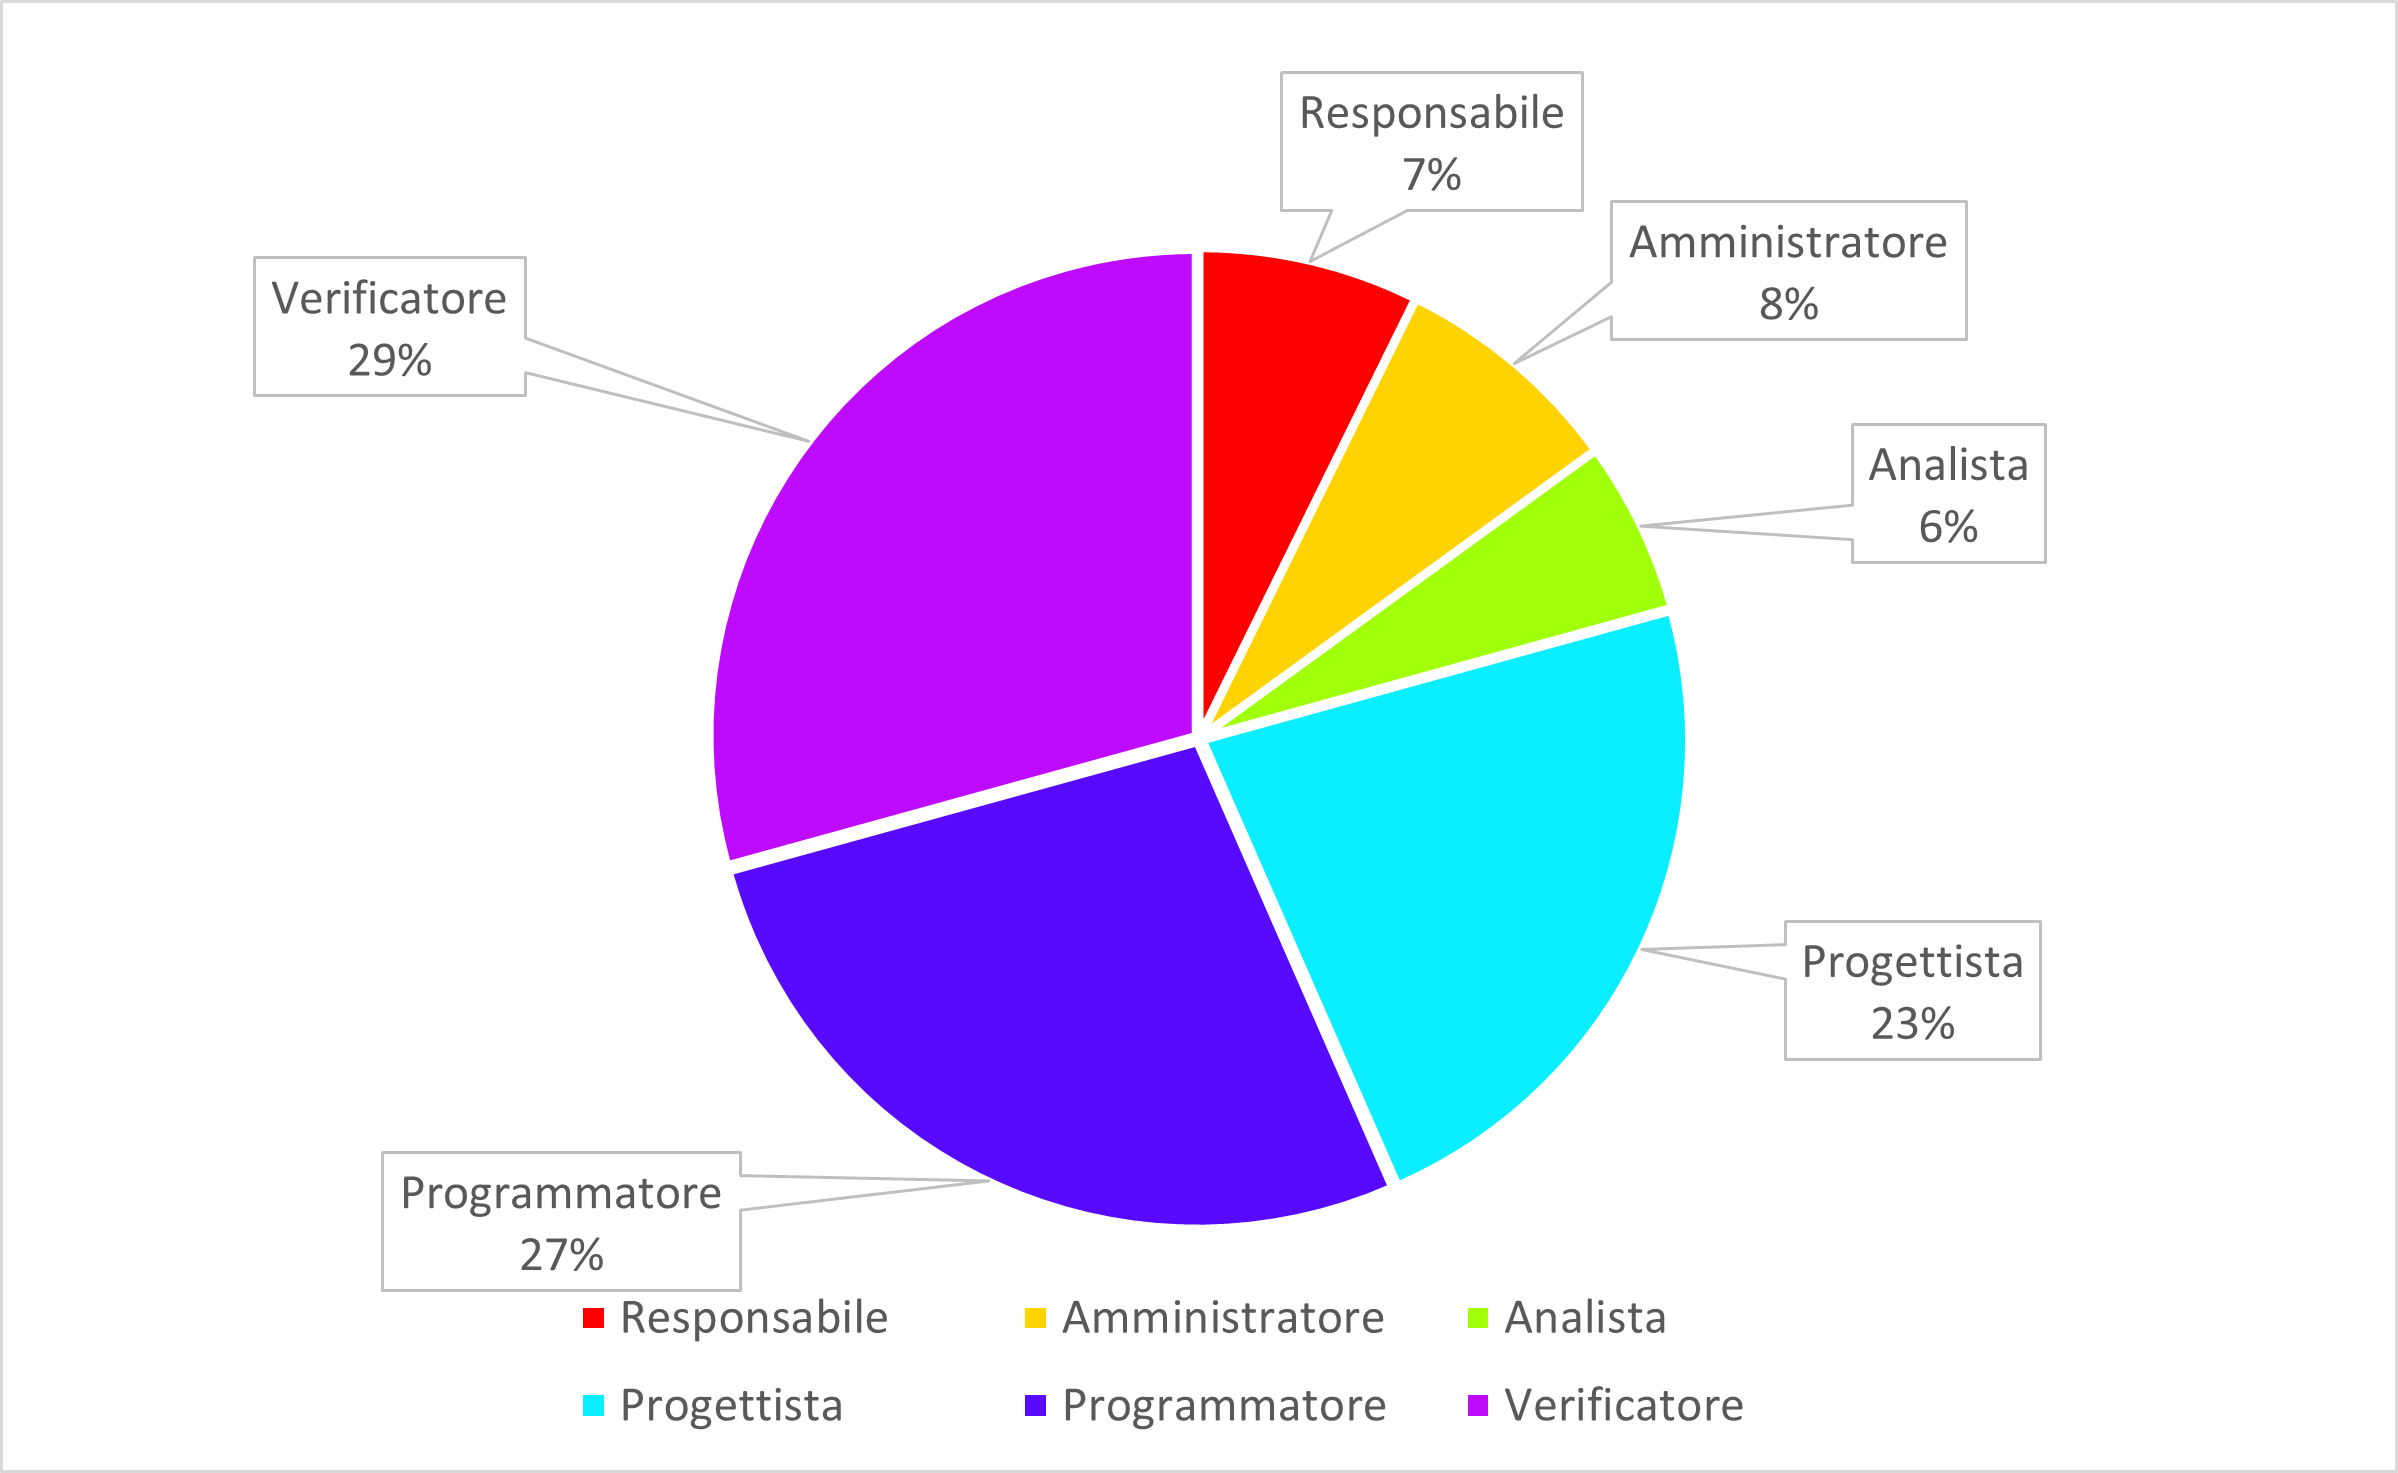
\includegraphics[scale = 0.5]{components/img/Totale-rendicontate-torta.png}
    \caption{Areogramma delle ore rendicontate per ruolo}
    \label{fig:Areogramma ripartizione ore totali rendicontate}
\end{figure}
\subsubsection{Conclusioni}
il costo totale preventivato è : 13048 \euro .
\newpage
\section{Consuntivo}
Di seguito verranno elencate le spese effettivamente sostenute per ogni ruolo. Il bilancio potrà essere:
\begin{itemize}
\item \textbf{Positivo:} se il preventivo supera il consuntivo;
\item \textbf{Pari:} se il consuntivo e il preventivo sono pari;
\item \textbf{Negativo:} se il consuntivo supera il preventivo.
\end{itemize}

\subsection{Periodo di Analisi}
Le ore di lavoro sostenute in questo periodo sono considerate come ore di investimento, motivo per il quale esse non vengono rendicontate.
\begin{table}[H]
		\begin{center}
			\setlength{\aboverulesep}{0pt}
			\setlength{\belowrulesep}{0pt}
			\setlength{\extrarowheight}{.75ex}
			\rowcolors{2}{AzzurroGruppo!10}{white}
			\begin{tabular}{ c c c }
				\rowcolor{AzzurroGruppo!30} 
				\textbf{Ruolo} & \textbf{Ore} & \textbf{Costo}  \\
				\toprule
				Responsabile & 29 & 870 \euro \\
				Amministratore & 35(+3) & 700\euro(+60\euro) \\
				Analista & 94(+10) & 2350\euro(+250\euro) \\
				Progettista & - & - \\
				Programmatore & - & - \\
				Verificatore & 70(+5) & 1050\euro(+75\euro) \\
				\textbf{Totale Preventivo} & \textbf{210} & \textbf{4585 \euro} \\
				\textbf{Totale Consuntivo} & \textbf{228} & \textbf{4970 \euro} \\
				\textbf{Differenza} & \textbf{18} & \textbf{385 \euro} \\
				\bottomrule
			\end{tabular}
			\caption{ Consuntivo della fase di analisi }
		\end{center}
\end{table}

\subsection{Conclusioni}
Come emerge dai dati riportati nella tabella soprastante, è stato necessario investire più tempo nei ruoli di \adm{}, \ana{} e \ver{}. Il bilancio risultante è negativo e di seguito sono spiegati i motivi:
\begin{itemize}
\item \textbf{Amministratore:} sono state aggiunte ed aggiornate alcune sezioni nelle \NdP{}, per chiarire alcune problematiche riscontrare durante la stesura dei documenti;
\item \textbf{Analista:} alcuni requisiti si sono rilevati di non facile comprensione, dunque sono state impiegate un maggior numero di ore lavorative per la discussione interna;
\item \textbf{Verificatore:} l'aggiunta di nuove sezioni nelle \NdP{} e il numero di requisiti trovati hanno richiesto più ore di lavoro anche per questo ruolo.
\end{itemize}
\newpage
\section{Organigramma}

\subsection{Redazione}

\renewcommand{\arraystretch}{1}
	\begin{table}[H]
		\begin{center}
			\setlength{\aboverulesep}{0pt}
			\setlength{\belowrulesep}{0pt}
			\setlength{\extrarowheight}{.75ex}
			\rowcolors{2}{AzzurroGruppo!10}{white}
			\begin{tabular}{ c c c }
				\rowcolor{AzzurroGruppo!30} 
				\textbf{Nome} & \textbf{Data Redazione} & \textbf{Firma} \\
				\toprule
				
				\Matteo{} & 2020-12-01 & 
\includegraphics[scale = 0.12]{components/img/firme_membri/firma-mp.png} \\
				\Tommaso{} & 2020-12-01 & 
\includegraphics[scale = 0.5]{components/img/firme_membri/firma-tp.png} \\
				
				\bottomrule
			\end{tabular}
			\caption{Redazione}
		\end{center}
	\end{table}

\subsection{Approvazione}

\renewcommand{\arraystretch}{1}
	\begin{table}[H]
		\begin{center}
			\setlength{\aboverulesep}{0pt}
			\setlength{\belowrulesep}{0pt}
			\setlength{\extrarowheight}{.75ex}
			\rowcolors{2}{AzzurroGruppo!10}{white}
			\begin{tabular}{ c c c}
				\rowcolor{AzzurroGruppo!30} 
				\textbf{Nome} & \textbf{Data Approvazione} & \textbf{Firma} \\
				\toprule
				
				\Daniele{} & 2021-01-10 & 
\includegraphics[scale = 0.16]{components/img/firme_membri/firma-dg.png} \\
				\Tullio{} & & \\
				\Riccardo{} & & \\
				
				\bottomrule
			\end{tabular}
			\caption{Approvazione}
		\end{center}
    \end{table}

\subsection{Accettazione componenti}

\renewcommand{\arraystretch}{1}
	\begin{table}[H]
		\begin{center}
			\setlength{\aboverulesep}{0pt}
			\setlength{\belowrulesep}{0pt}
			\setlength{\extrarowheight}{.75ex}
			\rowcolors{2}{AzzurroGruppo!10}{white}
			\begin{tabular}{ c c c}
				\rowcolor{AzzurroGruppo!30} 
				\textbf{Nome} & \textbf{Data Accettazione} & \textbf{Firma} \\
				\toprule
				
				\Davide{} & 2021-01-09 & 
\includegraphics[scale = 0.5]{components/img/firme_membri/firma-da.png} \\
				\Giosue{} & 2021-01-09 & 
\includegraphics[scale = 0.5]{components/img/firme_membri/firma-gc.png} \\
				\Francesco{} & 2021-01-09 & 
\includegraphics[scale = 0.16]{components/img/firme_membri/firma-fdm.png} \\
				\Daniele{} & 2021-01-09 & 
\includegraphics[scale = 0.16]{components/img/firme_membri/firma-dg.png} \\
				\Lucrezia{} & 2021-01-09 & 
\includegraphics[scale = 0.5]{components/img/firme_membri/firma-lg.png} \\
				\Matteo{} & 2021-01-09 & 
\includegraphics[scale = 0.12]{components/img/firme_membri/firma-mp.png} \\
				\Tommaso{} & 2021-01-09 & 
\includegraphics[scale = 0.5]{components/img/firme_membri/firma-tp.png} \\
				
				\bottomrule
			\end{tabular}
			\caption{Accettazione componenti}
		\end{center}
    \end{table}

\subsection{Componenti}

\renewcommand{\arraystretch}{1}
	\begin{table}[H]
		\begin{center}
			\setlength{\aboverulesep}{0pt}
			\setlength{\belowrulesep}{0pt}
			\setlength{\extrarowheight}{.75ex}
			\rowcolors{2}{AzzurroGruppo!10}{white}
			\begin{tabular}{ c c c }
				\rowcolor{AzzurroGruppo!30} 
				\textbf{Nome} & \textbf{Matricola} & \textbf{Indirizzo email}\\
				\toprule
				
				\Davide{} & 1193425 & davide.albiero@studenti.unipd.it \\
				\Giosue{} & 1201244 & giosue.calgaro@studenti.unipd.it \\
				\Francesco{} & 1201190 & francesco.demarchi.5@studenti.unipd.it \\
				\Daniele{} & 1201145 & daniele.giachetto@studenti.unipd.it \\
				\Lucrezia{} & 1142606 & lucrezia.gradi@studenti.unipd.it \\
				\Matteo{} & 1100806 & matteo.pagotto.1@studenti.unipd.it \\
				\Tommaso{} & 1201270 & tommaso.poppi@studenti.unipd.it \\
				
				\bottomrule
			\end{tabular}
			\caption{Componenti}
		\end{center}
    \end{table}
\newpage
\appendix

\section{Attualizzazione dei rischi}

In questa sezione vengono mostrate, sotto forma di tabella, tutte le contromisure adottate dal gruppo \gruppo{} riguardanti i rischi effettivamente riscontrati durante lo svolgimento del lavoro.  Per riuscire ad avere riscontro sull'efficacia delle contromisure prese, il gruppo ha deciso di adottare uno strumento di valutazione basato su tre livelli:

\setlength{\freewidth}{\dimexpr\textwidth-0\tabcolsep}
	\renewcommand{\arraystretch}{1.5}
	\setlength{\aboverulesep}{0pt}
	\setlength{\belowrulesep}{0pt}
	\rowcolors{2}{AzzurroGruppo!10}{white}
	\begin{longtable}{L{.210\freewidth} L{.6\freewidth} }
		\toprule 
		\rowcolor{AzzurroGruppo!30}
		\textbf{Nome} & \textbf{Descrizione} \\
		\hline
		\textbf{Bassa} & La contromisura non si è rivelata sufficiente e non è riuscita a mitigare al meglio il rischio riscontrato \\
		\textbf{Media} & La contromisura si è rivelata sufficiente a mitigare alcuni aspetti del rischio riscontrato. \\
		\textbf{Alta} & La contromisura si è rivelata sufficiente a mitigare molti o tutti gli aspetti del rischio riscontrato.\\
		\endhead		
		\hiderowcolors
		\caption{Descrizione livelli di efficacia contromisura }
	\end{longtable}

\subsection{Progettazione architetturale}

\setlength{\freewidth}{\dimexpr\textwidth-0\tabcolsep}
	\renewcommand{\arraystretch}{1.5}
	\setlength{\aboverulesep}{0pt}
	\setlength{\belowrulesep}{0pt}
	\rowcolors{2}{AzzurroGruppo!10}{white}
	\begin{longtable}{L{.210\freewidth} L{.6\freewidth} L{.1\freewidth}}
		\toprule 
		\rowcolor{AzzurroGruppo!30}
		\multicolumn{3}{c}{Rischi legati alle tecnologie}\\
		\toprule
		\textbf{Rischio} & \textbf{Mitigazione} & \textbf{Efficacia} \\
		\hline
		Inesperienza tecnologica & Durante la fase di apprendimento delle tecnologie necessarie allo sviluppo del \glo{Proof of Concept} sono stati riscontrati dei problemi. Questi si sono risolti grazie a continue comunicazioni col \glo{proponente} e al lavoro di gruppo, affiancato a materiale aggiuntivo da studiare singolarmente. & Alta\\
		\endhead		
		\hiderowcolors
		\caption{Attualizzazione per rischi legati alle tecnologie nel periodo di progettazione architetturale }
	\end{longtable}
	


\setlength{\freewidth}{\dimexpr\textwidth-0\tabcolsep}
	\renewcommand{\arraystretch}{1.5}
	\setlength{\aboverulesep}{0pt}
	\setlength{\belowrulesep}{0pt}
	\rowcolors{2}{AzzurroGruppo!10}{white}
	\begin{longtable}{L{.210\freewidth} L{.6\freewidth} L{.1\freewidth}}
		\toprule 
		\rowcolor{AzzurroGruppo!30}
		\multicolumn{3}{c}{Rischi legati all'organizzazione}\\
		\toprule
		\textbf{Rischio} & \textbf{Mitigazione} & \textbf{Efficacia}\\
		\hline
		Inesperienza gestionale & Si è riscontrato una differenza tra l'ammontare di ore stabilite per il lavoro e quelle effettivamente dovuto alle modifiche dei vari documenti e alla preparazione del \glo{Proof of Concept}. Questo ha spinto il gruppo alla ridistribuzione del carico di lavoro in modo da non rischiare ritardi.  & Bassa\\
		Interpretazione errata o cambio dei \glo{requisiti} & In seguito alle osservazioni fatte dopo la \textit{Revisione dei \ignore{Requisiti}}, il gruppo ha riscontrato gli errori svolti nell'\textit{Analisi dei \ignore{Requisiti}} e ha provveduto ad apportare le opportune modifiche e riempire le mancanze segnalate con priorità elevata. & Media\\
		
		\endhead		
		\hiderowcolors
		\caption{Attualizzazione per rischi legati all'organizzazione nel periodo di progettazione architetturale }
	\end{longtable}
	

\setlength{\freewidth}{\dimexpr\textwidth-0\tabcolsep}
	\renewcommand{\arraystretch}{1.5}
	\setlength{\aboverulesep}{0pt}
	\setlength{\belowrulesep}{0pt}
	\rowcolors{2}{AzzurroGruppo!10}{white}
	\begin{longtable}{L{.210\freewidth} L{.6\freewidth} L{.1\freewidth}}
		\toprule 
		\rowcolor{AzzurroGruppo!30}
		\multicolumn{3}{c}{Rischi legati alle persone}\\
		\toprule
		\textbf{Rischio} & \textbf{Mitigazione} & \textbf{Efficacia} \\
		\hline
		Impegni personali & Durante il periodo i membri del gruppo si sono trovati a svolgere la sessione d'esame. Per assicurare la continuità del progetto il carico di lavoro è stato ridistribuito tra i membri con più disponibilità.  & Alta\\
		\endhead		
		\hiderowcolors
		\caption{Attualizzazione per rischi legati alle persone nel periodo di progettazione architetturale }
	\end{longtable}
	

\subsection{Progettazione di dettaglio e codifica}


	
	\setlength{\freewidth}{\dimexpr\textwidth-0\tabcolsep}
	\renewcommand{\arraystretch}{1.5}
	\setlength{\aboverulesep}{0pt}
	\setlength{\belowrulesep}{0pt}
	\rowcolors{2}{AzzurroGruppo!10}{white}
	\begin{longtable}{L{.210\freewidth} L{.6\freewidth} L{.1\freewidth}}
		\toprule 
		\rowcolor{AzzurroGruppo!30}
		\multicolumn{3}{c}{Rischi legati all'organizzazione}\\
		\toprule
		\textbf{Rischio} & \textbf{Mitigazione} & \textbf{Efficacia}\\
		\hline
		Inesperienza gestionale & La mitigazione del periodo precedente, cioè la ridistribuzione del carico di lavoro, non si è dimostrata efficace a contenere i ritardi. Per questo si è deciso di redigere una \glo{timeline} in modo da avere una più chiara visione d'insieme di ciò che va fatto e di chi è disponibile in quel determinato lasso di tempo. Grazie all'introduzione della suddetta \glo{timeline} e agli obiettivi di \glo{sprint} i ritardi sono stati efficacemente contenuti e si è riuscito a ottenere un buon livello di organizzazione. & Alta\\
		
		\endhead		
		\hiderowcolors
		\caption{Attualizzazione per rischi legati all'organizzazione nel periodo di progettazione di dettaglio e codifica }
	\end{longtable}
	
\subsection{Validazione e collaudo}
	
	\setlength{\freewidth}{\dimexpr\textwidth-0\tabcolsep}
	\renewcommand{\arraystretch}{1.5}
	\setlength{\aboverulesep}{0pt}
	\setlength{\belowrulesep}{0pt}
	\rowcolors{2}{AzzurroGruppo!10}{white}
	\begin{longtable}{L{.210\freewidth} L{.6\freewidth} L{.1\freewidth}}
		\toprule 
		\rowcolor{AzzurroGruppo!30}
		\multicolumn{3}{c}{Rischi legati alle tecnologie}\\
		\toprule
		\textbf{Rischio} & \textbf{Mitigazione} & \textbf{Efficacia}\\
		\hline
		Problematiche Hardware & Sono stati riscontrati malfunzionamenti sull'unico computer avente come sistema operativo macOS. Questo poteva intaccare lo sviluppo e testing in locale su quel sistema operativo. Fortunatamente le problematiche erano note al gruppo da tempo e si è riusciti a procurare un computer di ricambio poco dopo la rottura del primo.  & Alta\\
		Problematiche Software & Per rilasciare l'eseguibile dell'applicativo per i vari sistemi operativi ci si è imbattuti in diverse problematiche con i programmi utilizzati per effettuare il rilascio. Si sono presentati diversi problemi nati dall'utilizzo di Qt6 ed il gruppo ha dovuto dedicare diverse ore per studiare metodi alternativi per il rilascio, riuscendo infine ad effettuarlo gestendo manualmente le librerie da utilizzare.  & Alta\\
		\endhead		
		\hiderowcolors
		\caption{Attualizzazione per rischi legati alle tecnologie nel periodo di validazione e collaudo }
	\end{longtable}
	
	
		\setlength{\freewidth}{\dimexpr\textwidth-0\tabcolsep}
	\renewcommand{\arraystretch}{1.5}
	\setlength{\aboverulesep}{0pt}
	\setlength{\belowrulesep}{0pt}
	\rowcolors{2}{AzzurroGruppo!10}{white}
	\begin{longtable}{L{.210\freewidth} L{.6\freewidth} L{.1\freewidth}}
		\toprule 
		\rowcolor{AzzurroGruppo!30}
		\multicolumn{3}{c}{Rischi legati alle persone}\\
		\toprule
		\textbf{Rischio} & \textbf{Mitigazione} & \textbf{Efficacia}\\
		\hline
		Impegni personali & Durante questo periodo alcuni membri del gruppo, per via di impegni personali e lavorativi, non sono riusciti a dedicare abbastanza tempo al progetto; questo ha fatto si che il lavoro si accumulasse. Per risolvere è stato ridistribuito il lavoro tra i membri con più disponibilità.& Alta\\
		
		\endhead		
		\hiderowcolors
		\caption{Attualizzazione per rischi legati alle persone nel periodo di validazione e collaudo }
	\end{longtable}
	
\newpage

\end{document}